\chapter{Differential Cross Sections: Data, Simulation and Selection}
\label{c:Differential_Cross_Section:data_simulation_and_selection}

\section{Outline and Motivation}
\label{s:outline_and_motivation}
This chapter describes the first part of the main \ttbar differential cross section analysis in bins of global
event variables. Following an introduction to the variables under investigation and motivations, the datasets
used and the selection process is explained, including scale factors and corrections applied to ensure
agreement between Monte Carlo simulation and data.

The analysis measures the normalised differential \ttbar cross section in the semi-leptonic channel and is
carried out on 2011 and 2012 data recorded from the CMS detector. The measurement is carried out with respect
to the following global, or primary, variables:
\begin {itemize}

  \item {\met, the missing transverse energy in an event, defined as the magnitude of the missing transverse
  momentum vector \ptvecmiss (which is defined as the projection of the negative vector sum of the momenta of
  all PF objects in the event on the plane perpendicular to the beams).}
  	\[\met = \left[ \left(\sum_i{p_{x}^i}\right)^2 + \left(\sum_i{p_{y}^i}\right)^2 \right]^{\frac{1}{2}},\]
  	where $p_x^i$ and $p_yi$ are momentum components of the \textit{i}th object in the event, and the sums
  	include all PF objects in the event, with no lower threshold applied. See Section~\ref{ss:met_corrections}
  	for details of corrections applied in the calculation of this \met, which include, amongst others,
  	propagation of jet energy corrections and takes account of pileup interactions.

  \item {\HT, the sum of the transverse momenta of all jets with $\pt>20\GeV$ and $\abseta<2.5$ in an
  event}
  	\[\HT = \sum_{\text{all jets}}\pt^{\mathrm{jet}}\].

  \item {\st, the sum of all observed transverse momenta in an event, \ie the scalar sum of \HT, \met, and
  	lepton \pt}
  	\[\st = \HT + \met + p_\mathrm{T}^\mathrm{lepton}.\]

  \item {\wpt, the transverse momentum of the leptonically decaying \W boson, obtained from \ptvecmiss and the
  \pt of the lepton}
	\[\wpt = \sqrt{\left(p_x^{\mathrm{lepton}} + p_x^{\mathrm{miss}}\right)^2 + \left(p_y^{\mathrm{lepton}} +
	p_y^{\mathrm{miss}}\right)^2},\]
	where $p_{x}^{\mathrm{lepton}}$ and $p_{y}^{\mathrm{lepton}}$ are the transverse components of
	$\vec{p}^{\mathrm{lepton}}$, and $p_x^{\mathrm{miss}}$ and $p_y^{\mathrm{miss}}$ are the transverse
	components of \ptvecmiss.

  \item {\mt, the transverse mass of the leptonically decaying \W boson, also obtained from \met and the \pt
  of the lepton}
    \[\mt = \sqrt{\et\left(\text{lepton}, \met\right)^{2} - (\wpt)^{2}},\]
    where $\et\left(\text{lepton}, \met\right)$ is the scalar sum of \met and the transverse energy of the
    lepton, \ie $\met + \et^{\text{lepton}}$
 
\end{itemize}

The central objective of these measurements is to verify the models and generators used to produce simulations
of the signal and background events in CMS. This understanding is important to provide a good foundation for
new physics analyses, where such events constitute a significant background. Comparison of results with
predictions using varied choices of the matching threshold of partons, and the renormalisation and
factorisation scale ($Q^{2}$) allow the verification of these model parameters used in event generation. In
addition, the distributions under investigation may be sensitive to rare standard model processes; for
example, the \met and \mt distributions could show signs of \ttbar+\Z (where $Z\rightarrow \nu\bar{\nu}$)
and/or \ttbar+\W (where $W\rightarrow l\nu$) processes, which produce additional \met. The \wpt and \mt
distributions are related to the leptonically decaying \W boson, and therefore give a handle on modelling of
the transverse momentum of the relevant top quark. The \HT and \st distributions would provide information on
\ttbar+X production where X is massive and decays to hadrons. Hints of new physics scenarios such as stop pair
production, $\tilde{t}\bar{\tilde{t}} \rightarrow t\tilde{\chi_0} \bar{t}\bar{\tilde{\chi_0}}$, where
$\tilde{\chi_0}$ is the lightest supersymmetric particle and a possible dark matter candidate, may also be
visible in the distributions of global variables. Cases of rare SM processes or new physics are likely to
manifest as observed excesses over predictions in the tails of the primary variables, making this region of
the distributions of particular interest.

Note that this analysis on the aforementioned global variables does not require reconstruction of the \ttbar
decay to identify which decay products are associated with each top quark, and is intended as a complementary
analysis to other CMS studies in which such reconstruction is carried out.

\section{Data and Simulated Samples}
\label{s:data_and_simulated_samples}

\subsection{Data}
\label{ss:data}

Data collected in 2011 at a centre-of-mass energy of 7\TeV corresponding to an integrated luminosity of
5.0\fbinv, and in 2012 at a centre-of-mass energy of 8\TeV corresponding to an integrated luminosity of
19.7\fbinv are used in this analysis. The datasets are determined by the triggers that were used to record
them. For 7\TeV, the ``ElectronHad'' dataset is used in the electron channel, which was recorded with triggers
that select events based on at least one, isolated electron and additional jets. At 8\TeV, the
``SingleElectron'' dataset was used for the electron channel which is based only on at least one, isolated
electron. In the muon channel, the ``SingleMu'' dataset was used for both centre-of-mass energies, requiring a
single, isolated muon.

These datasets are produced from CMS data by requiring events to pass a trigger. The triggers used in both
7\TeV and 8\TeV data are shown in Table~\ref{tab:HLTTriggers} in Appendix~\ref{as:datasets}. In the electron
channel, an electron+jets trigger was used in 2011 with a requirement of at least one electron with
\Et$>25\GeV$ and at least three jets with \pt$>30\GeV$; and a single electron trigger was used in 2012 with at
least one electron with \Et$>27\GeV$. In the muon channel, a single muon trigger was used in both data taking
periods with a requirement of at least one muon with \pt$>24\GeV$. In addition to these kinematic
requirements, the triggers also have cuts on the ratio between the HCAL and the ECAL energy ($H/E$), track matching with
ECAL ($\Delta\eta$ and $\Delta\phi$), cluster shape ($\sigma_{i\eta i\eta}$), ECAL isolation
($\frac{\text{ECAL iso}}{E_\text{T}}$), HCAL isolation ($\frac{\text{HCAL iso}}{E_\text{T}}$) and tracker
isolation ($\frac{\text{tracker iso}}{\pt}$). In both channels, the final selection is tighter than these
trigger requirements.

The datasets used are shown in Tables~\ref{tab:datasets7TeV} and \ref{tab:datasets8TeV}.Only data that is
certified as ``golden'' (data taken with the CMS detector working without any major faults) is used. The masks
used to filter out data taken in other periods are specified in Table~\ref{tab:JSONfiles} in
Appendix~\ref{as:datasets}.

\begin{table}[hbth]
\centering
\begin{tabular}{llrr}
\hline
\textbf{Data set name} & \textbf{Run period} & \textbf{$\mathbf{\mathcal{L}_{int}}$ / \pbinv} & \textbf{Runs}
\\
\hline
ElectronHad 12 Oct 2013 ReReco & Run2011A & 2,333 & 160404--173692 \\
ElectronHad 12 Oct 2013 ReReco & Run2011B & 2,738 & 175833--180252 \\
\hline
SingleMu 12 Oct 2013 ReReco & Run2011A & 2,331 & 160404--173692 \\
SingleMu 12 Oct 2013 ReReco & Run2011B & 2,766 & 175833--180252 \\
\hline
\end{tabular}
\caption{7 TeV data sets by run period with the corresponding integrated
luminosities ($\mathcal{L}_{int}$) and run numbers.}
\label{tab:datasets7TeV}
\end{table}
\begin{table}[hbth]
\centering
\begin{tabular}{llrr}
\hline
\textbf{Data set name} & \textbf{Run period} & \textbf{$\mathbf{\mathcal{L}_{int}}$ / \pbinv} & \textbf{Runs}
\\
\hline
SingleElectron 22 Jan 2013 ReReco & Run2012A & $883.3$ & 190456--193621 \\
SingleElectron 22 Jan 2013 ReReco & Run2012B & $4,389.0$ & 193834--196531 \\
SingleElectron 22 Jan 2013 ReReco & Run2012C & $7,137.0$ & 198022--203742 \\
SingleElectron 22 Jan 2013 ReReco & Run2012D & $7,318.0$ & 203777--208686 \\
\hline
SingleMu 22 Jan 2013 ReReco & Run2012A & $889.4$ & 190456--193621 \\
SingleMu 22 Jan 2013 ReReco & Run2012B & $4,424.0$ & 193834--196531 \\
SingleMu 22 Jan 2013 ReReco & Run2012C & $7,152.0$ & 198022--203742 \\
SingleMu 22 Jan 2013 ReReco & Run2012D & $7,280.0$ & 203777--208686 \\
\hline
\end{tabular}
\caption{8 TeV data sets by run period with the corresponding integrated
luminosities ($\mathcal{L}_{int}$) and run numbers.}
\label{tab:datasets8TeV}
\end{table}

\FloatBarrier

\subsection{Simulated Samples}
\label{ss:simulated_samples}
The signal event for this analysis is the production of a \ttbar pair which decays semi-leptonically, \ie each
of the \tquarks decays to a \W boson and a \bjet, with one of the \W bosons decaying hadronically to two jets
and the other decaying leptonically to a lepton (electron or muon) and an associated neutrino.
Section~\ref{c:top_physics_at_the_lhc} outlines the signal and background events considered. Additional, lower
energy jets, can be produced from other scatterings in the same proton-proton interaction and from gluon
radiation from quarks in the decay. See Section~\ref{c:top_physics_at_the_lhc} for detailed descriptions of
the signal and backgrounds in this analysis.

The Monte Carlo generators used in this analysis are \MADGRAPH v5.1.5.11~\cite{madgraph5}, \PYTHIA
v6.426~\cite{Sjostrand:2006za}, \POWHEG v1.0, r1380 and \POWHEG v2.0,
r2819~\cite{Nason:2004rx,Frixione:2007vw,Alioli:2010xd}, \HERWIG v6.520~\cite{herwig} and \MCATNLO
v3.41~\cite{Frixione:2002ik,Frixione:2003ei}. See Section~\ref{s:monte_carlo_simulation} for details about
these Monte Carlo generators. The \GEANTfour package~\cite{Agostinelli:2002hh,Allison:2006ve} is used to
simulate the CMS detector response.

Tables~\ref{tab:signaldatasets7TeV} and~\ref{tab:signaldatasets8TeV} show the Monte Carlo signal samples used
in this analysis at 7\TeV and 8\TeV respectively. Tables~\ref{tab:backgrounddatasets7TeV}
and~\ref{tab:backgrounddatasets8TeV} list the background simulation samples used.

Top pair production is modelled using the \MADGRAPH event generator, with \PYTHIA modelling the parton
showering and hadronisation, with matching between the parton showers and the matrix element performed via the
MLM prescription~\cite{Hoche:2006ph} (Section~\ref{ss:madgraph}). Two independent \ttbar samples are also
produced with the \POWHEG2 generator interfaced with \PYTHIA and \HERWIG for parton showering. At
$\roots=7\TeV$, three additional samples are used generated using \MCATNLO with \HERWIG to model the parton
showers, \POWHEG1 with \PYTHIA, and \POWHEG1 with \HERWIG.

Single top events are modelled with \POWHEG, \W and \Z boson plus jets production is modelled using \MADGRAPH
and QCD multi-jet events are modelled with \PYTHIA. Tables~\ref{tab:7TeVsystematicdatasets} and
\ref{tab:8TeVsystematicdatasets} show the samples used to evaluate the factorisation scale, matching
threshold, and top quark mass uncertainties. \WpJets and \ZpJets samples were not made available at 7\TeV, so
the scaled distributions from 8\TeV were used, as described in
Section~\ref{sss:7TeV_vjets_theory_systematic_template}.

Standard Model cross sections at NNLO of 252.89\pb at $\roots=7\TeV$ and 177.31\pb at $\roots=8\TeV$ are used
for \ttbar processes~\cite{Czakon:2013goa}. NNLO cross sections are also applied for\WpJets processes and
\ZpJets processes~\cite{Melnikov:2006kv}. Cross sections at NLO are used for single top
processes~\cite{Campbell:2009ss} and LO cross sections are used for QCD multi-jet processes. Numerical values
for cross sections are included in all abovementioned tables.

The CTEQ6L PDFs~\cite{Pumplin:2002vw} are used to generate the \MADGRAPH simulations, the CT10
PDFs~\cite{ct10} are used for \POWHEG production and CTEQ6M PDFs~\cite{Pumplin:2002vw} are used for \MCATNLO.
The underlying event tunes (sets of theory parameters) used for production of the \MADGRAPH and \POWHEGPYTHIA2
samples at $\roots=7\TeV$, as well as the \MCATNLOHERWIG sample at $\roots=8\TeV$, is the \PYTHIA Z2
tune~\cite{Z2UE}. The \PYTHIA Z2* is used for the \MADGRAPH, \POWHEGPYTHIA1 and \POWHEGPYTHIA2 samples at
$\roots=8\TeV$, and the AUET tune~\cite{AUET2UE} is used in all \POWHEGHERWIG samples. All simulations are
generated with a top quark mass of 172.5\GeV, and in all cases, \PYTHIA is used to model parton showering,
radiation and hadronisation processes.

\begin{table}[hbth]
\centering
\caption{7\TeV Monte Carlo signal datasets used for this analysis.}
\label{tab:signaldatasets7TeV} \small\addtolength{\tabcolsep}{-5pt}
\begin{tabular}{llrrr}
%\multicolumn{6}{c}{Signal datasets}
%\hline
Process & Generator & $\sigma$/$\pb$ & No. events & \lumiint/$\fbinv$ \\
\hline
\ttbar & \MADGRAPH & 177.31 & 17100187 & 96.4 \\
\ttbar & \MCATNLO & Not Available & - & - \\
\ttbar & \POWHEGPYTHIA1 & Not Available & - & - \\
\ttbar & \POWHEGHERWIG1 & Not Available & - & - \\
\ttbar & \POWHEGPYTHIA2 & 177.31 & 4833135 & 27.3 \\
\ttbar & \POWHEGHERWIG2 & 177.31 & 4480816 & 25.3 \\
\hline
\end{tabular}
\end{table}


\begin{table}[hbth]
\centering
\caption{8\TeV Monte Carlo signal datasets used for this analysis.}
\label{tab:signaldatasets8TeV} \small\addtolength{\tabcolsep}{-5pt}
\begin{tabular}{llrrr}
%\multicolumn{6}{c}{Signal datasets}
%\hline
Process & Generator & $\sigma$/$\pb$ & No. events & \lumiint/$\fbinv$ \\
\hline
\ttbar & \MADGRAPH & 252.89 & 6706068 & 26.5 \\
\ttbar & \MCATNLO & 252.89 & 32852517 & 129.9 \\
\ttbar & \POWHEGPYTHIA1 & 252.89 & 21675913 & 85.7 \\
\ttbar & \POWHEGHERWIG1 & 252.89 & 27684194 & 109.5 \\
\ttbar & \POWHEGPYTHIA2 & 252.89 & 9044049 & 35.8 \\
\ttbar & \POWHEGHERWIG2 & 252.89 & 8630382 & 34.1 \\
\hline
\end{tabular}
\end{table}


\begin{table}[hbth]
\centering
\caption{\SI{7}{\TeV} Monte Carlo background datasets used for this analysis. All samples are generated
inclusively if not marked otherwise ($^\star$ generator cut on in-flight-decays of b- and c-hadrons, $^\ominus$ enriched in conversion electrons; $l$ means
all leptonic decays: $l=e,\mu,\tau$; $^\bullet$ generator cut on $m_{Z/\gamma} > 50$~GeV).
\label{tab:backgrounddatasets7TeV}} \small\addtolength{\tabcolsep}{-5pt}
\begin{tabular}{llrrr}
%\multicolumn{6}{c}{Background datasets} 
%\hline
Process & Generator & $\sigma$ ($\pb$) & No. events & \lumiint ($\fbinv$) \\
\hline
\hline
Single \cPqt t-channel ($W\rightarrow l\nu$) & \POWHEG & 42.6 & 3249530 & 76.3 \\
Single \cPaqt t-channel ($W\rightarrow l\nu$) & \POWHEG & 22.0 & 1813615 & 82.4 \\
Single \cPqt s-channel ($W\rightarrow l\nu$) & \POWHEG & 2.72 & 229786 & 84.5 \\
Single \cPaqt s-channel ($W\rightarrow l\nu$) & \POWHEG & 1.49 & 138187 & 92.7 \\
Single \cPqt tW-channel ($W\rightarrow l\nu$) & \POWHEG & 5.3 & 744859 & 140.5 \\
Single \cPaqt tW-channel ($W\rightarrow l\nu$) & \POWHEG & 5.3 & 801626 & 151.3 \\
\hline
\W ($\rightarrow l\nu$) + 1 Jet & \MADGRAPH & 4480.0 & 70430949 & 15.7 \\
\W ($\rightarrow l\nu$) + 2 Jets & \MADGRAPH & 1435.0 & 25069566 & 17.5 \\
\W ($\rightarrow l\nu$) + 3 Jets & \MADGRAPH & 304.2 & 6291772 & 20.7 \\
\W ($\rightarrow l\nu$) + 4 Jets & \MADGRAPH & 172.6 & 13240209 & 76.7 \\
\Z/$\photon^{*}$ ($\rightarrow l^+l^-$) + jets $^\bullet$ & \MADGRAPH & 3048 & 32846945 & 10.8 \\
\hline
QCD BCtoE \PT 20-30 $^\star$ & \PYTHIA & 139299.0 & 1927944 & 1.4$\times 10^{-2}$ \\
QCD BCtoE \PT 30-80 $^\star$ & \PYTHIA & 143844.8 & 1946505 & 1.4$\times 10^{-2}$ \\
QCD BCtoE \PT 80-170 $^\star$ & \PYTHIA & 9431.1 & 1002427 & 0.1 \\
\hline
QCD EM  \PT 20-30 $^\ominus$ & \PYTHIA & 2502660.0 & 32976415 & 1.3$\times 10^{-2}$ \\ 
QCD EM \PT 30-80 $^\ominus$ & \PYTHIA & 3625840.0 & 71775065 & 2.0$\times 10^{-2}$ \\
QCD EM \PT 80-170 $^\ominus$ & \PYTHIA & 142813.8 & 7650319 & 5.4$\times 10^{-2}$ \\
QCD EM  \PT 170-250 $^\ominus$ & \PYTHIA & 142813.8 & 2968842 & 2.1$\times 10^{-2}$ \\
QCD EM  \PT 250-350 $^\ominus$ & \PYTHIA & 368.0 & 2952960 & 8.0 \\
QCD EM \PT 350-inf $^\ominus$ & \PYTHIA & 55.0 & 2957326 & 53.8 \\
\hline
$\gamma$ + Jets HT 40-100 & \MADGRAPH & 25690.0 & 9882860 & 0.4 \\
$\gamma$ + Jets HT 100-200 & \MADGRAPH & 5213.0 & 1514347 & 0.3 \\
$\gamma$ + Jets HT $>$ 200 & \MADGRAPH & 798.3 & 9275592 & 11.6 \\
\hline
QCD $\mu$ enriched \PT 15-20 & \PYTHIA & 1668096.0 & 1901684 & 1.1$\times 10^{-3}$ \\
QCD $\mu$ enriched \PT 20-30 & \PYTHIA & 1342184.0 & 10173300 & 7.6$\times 10^{-3}$ \\
QCD $\mu$ enriched \PT 30-50 & \PYTHIA & 596506.8 & 11610111 & 1.9$\times 10^{-2}$ \\
QCD $\mu$ enriched \PT 50-80 & \PYTHIA & 140039.55 & 9870031 & 7.0$\times 10^{-2}$ \\
QCD $\mu$ enriched \PT 80-120 & \PYTHIA & 28546.2 & 9769136 & 0.3 \\
QCD $\mu$ enriched \PT 120-170 & \PYTHIA & 4692.91 & 7818474 & 1.7 \\
QCD $\mu$ enriched \PT 170-300 & \PYTHIA & 1445.96 & 8116409 & 5.6 \\
QCD $\mu$ enriched \PT 300-470 & \PYTHIA & 95.4464 & 7870002 & 82.5 \\
QCD $\mu$ enriched \PT 470-600 & \PYTHIA & 7.41697 & 3812529 & 514.0 \\
QCD $\mu$ enriched \PT 600-800 & \PYTHIA & 1.69145 & 4149911 & 2453.5 \\
QCD $\mu$ enriched \PT 800-1000 & \PYTHIA & 0.231869 & 4036867 & 17410.1 \\
QCD $\mu$ enriched \PT 1000-inf & \PYTHIA & 0.053385 & 4133897 & 77435.6 \\
\hline
\end{tabular}
\end{table}
\begin{table}[hbth]
\centering
\caption{\SI{8}{\TeV} Monte Carlo background datasets used for this analysis. All samples are generated
inclusively if not marked otherwise ($^\star$ generator cut on in-flight-decays of b- and c-hadrons, $^\ominus$ enriched in conversion electrons; $l$ means
all leptonic decays: $l=e,\mu,\tau$; $^\bullet$ generator cut on $m_{Z/\gamma} > 50$~GeV).
\label{tab:backgrounddatasets8TeV}} \small\addtolength{\tabcolsep}{-5pt}
\begin{tabular}{llrrr}
%\multicolumn{6}{c}{Background datasets} 
%\hline
Process & Generator & $\sigma$ ($\pb$) & No. events & \lumiint ($\fbinv$) \\
\hline
\hline
Single \cPqt t-channel ($W\rightarrow l\nu$) & \POWHEG & 55.53100 & 3758221 & 67.7 \\
Single \cPaqt t-channel ($W\rightarrow l\nu$) & \POWHEG & 30.00420 & 1906041 & 63.5 \\
Single \cPqt s-channel ($W\rightarrow l\nu$) & \POWHEG & 3.89394 & 259960 & 66.8 \\
Single \cPaqt s-channel ($W\rightarrow l\nu$) & \POWHEG & 1.75776 & 139974 & 79.6 \\
Single \cPqt tW-channel ($W\rightarrow l\nu$) & \POWHEG & 11.17730 & 497657 & 44.5 \\
Single \cPaqt tW-channel ($W\rightarrow l\nu$) & \POWHEG & 11.17730 & 473721 & 42.4 \\
\hline
\W ($\rightarrow l\nu$) + 1 Jet & \MADGRAPH & 5400.0 & 23129996 & 15.7 \\
\W ($\rightarrow l\nu$) + 2 Jets & \MADGRAPH & 1750.0 & 34027847 & 17.5 \\
\W ($\rightarrow l\nu$) + 3 Jets & \MADGRAPH & 519.0 & 15539463 & 20.7 \\
\W ($\rightarrow l\nu$) + 4 Jets & \MADGRAPH & 214.0 & 13373865 & 76.7 \\
\Z/$\photon^{*}$ ($\rightarrow l^+l^-$) + 1 jet$^\bullet$ & \MADGRAPH & 561.0 & 24032529 & 42.8 \\
\Z/$\photon^{*}$ ($\rightarrow l^+l^-$) + 2 jets$^\bullet$ & \MADGRAPH & 181.0 & 21840628 & 0.1 \\
\Z/$\photon^{*}$ ($\rightarrow l^+l^-$) + 3 jets$^\bullet$ & \MADGRAPH & 51.1 & 10819603 & 0.2 \\
\Z/$\photon^{*}$ ($\rightarrow l^+l^-$) + 4 jets$^\bullet$ & \MADGRAPH & 23.04 & 6381467 & 0.3 \\
\hline
QCD BCtoE \PT 20-30 $^\star$ & \PYTHIA & 167388.0 & 1731522 & 1.0$\times 10^{-2}$ \\
QCD BCtoE \PT 30-80 $^\star$ & \PYTHIA & 167040.0 & 2037907 & 1.2$\times 10^{-2}$ \\
QCD BCtoE \PT 80-170 $^\star$ & \PYTHIA & 12981.9 & 1945523 & 0.1 \\
QCD BCtoE \PT 170-250 $^\star$ & \PYTHIA & 632.0 & 1948112 & 3.1 \\
QCD BCtoE \PT 250-350 $^\star$ & \PYTHIA & 103.3 & 2026516 & 19.6 \\
QCD BCtoE \PT 350-inf $^\star$ & \PYTHIA & 23.9 & 1948525 & 81.5 \\
\hline
QCD EM  \PT 20-30 $^\ominus$ & \PYTHIA & 2914860.0 & 34830398 & 1.2$\times 10^{-2}$ \\ 
QCD EM \PT 30-80 $^\ominus$ & \PYTHIA & 4615893.0 & 32443607 & 7.0$\times 10^{-3}$ \\
QCD EM \PT 80-170 $^\ominus$ & \PYTHIA & 183294.9 & 34024542 & 0.2 \\
QCD EM  \PT 170-250 $^\ominus$ & \PYTHIA & 4586.5 & 31696985 & 6.9 \\
QCD EM  \PT 250-350 $^\ominus$ & \PYTHIA & 556.7 & 33659467 & 60.5 \\
QCD EM \PT 350-inf $^\ominus$ & \PYTHIA & 89.1 & 33756727 & 378.8 \\
\hline
$\gamma$ + Jets HT 200-400 & \MADGRAPH & 960.5 & 47316433 & 49.3 \\
$\gamma$ + Jets HT 400-inf & \MADGRAPH & 107.5 & 9491846 & 88.3 \\
\hline
QCD $\mu$ enriched \PT 15-20 & \PYTHIA & 2738580.0 & 1722678 & 0.6$\times 10^{-3}$ \\
QCD $\mu$ enriched \PT 20-30 & \PYTHIA & 1865500.0 & 8486893 & 4.5$\times 10^{-3}$ \\
QCD $\mu$ enriched \PT 30-50 & \PYTHIA & 806298.0 & 9560248 & 1.2$\times 10^{-2}$ \\
QCD $\mu$ enriched \PT 50-80 & \PYTHIA & 176187.6 & 10365209 & 5.9$\times 10^{-2}$ \\
QCD $\mu$ enriched \PT 80-120 & \PYTHIA & 40448.0 & 9238622 & 0.2 \\
QCD $\mu$ enriched \PT 120-170 & \PYTHIA & 7463.94 & 8501920 & 1.1 \\
QCD $\mu$ enriched \PT 170-300 & \PYTHIA & 2299.752 & 7669932 & 3.3 \\
QCD $\mu$ enriched \PT 300-470 & \PYTHIA & 151.8048 & 7832248 & 51.6 \\
QCD $\mu$ enriched \PT 470-600 & \PYTHIA & 11.79648 & 3783066 & 320.7 \\
QCD $\mu$ enriched \PT 600-800 & \PYTHIA & 2.690196 & 4118988 & 1531.1 \\
QCD $\mu$ enriched \PT 800-1000 & \PYTHIA & 0.3687810 & 4099633 & 11116.7 \\
QCD $\mu$ enriched \PT 1000-inf & \PYTHIA & 0.0849078 & 9238622 & 108807.7 \\
\hline
\end{tabular}
\end{table}

\begin{landscape}
\begin{table}[hbth]
\centering
\caption{7~\TeV Monte Carlo systematic datasets used for this analysis. All samples are produced with
the \MADGRAPH generator. \WpJets and \ZpJets samples were not available and so have been scaled from
available 8\TeV samples.}
\label{tab:7TeVsystematicdatasets} \small\addtolength{\tabcolsep}{-5pt}
\begin{tabular}{lllrrr}
%\multicolumn{6}{c}{Signal datasets}
%\hline
Process & Variation & Generator & $\sigma$ ($\pb$) & No. events & \lumiint ($\fbinv$) \\
\hline
\ttbar & 0.5$\times Q^{2}$ (norm. \& fact. scale down) & \MADGRAPH & 177.31 & 9426377 & 53.2
\\
\ttbar & 2$\times Q^{2}$ (norm. \& fact. scale up) & \MADGRAPH & 177.31 & 10095984 & 56.9 \\
\ttbar & 0.5$\times$matching threshold (down) & \MADGRAPH & 177.31 & 4056487 & 22.9 \\
\ttbar & 2$\times$matching threshold (up) & \MADGRAPH & 177.31 & 16727257 & 94.3 \\
\ttbar & 0.5$\times$mass uncertainty (down) & \MADGRAPH & 177.31 & 4560762 & 25.7 \\
\ttbar & 2$\times$mass uncertainty (up) & \MADGRAPH & 177.31 & 9151264 & 51.6 \\
\hline
\WpJets & 0.5$\times Q^{2}$ (norm. \& fact. scale down) & \MADGRAPH & 31314 & 20121177 & 0.6 \\
\WpJets & 2$\times Q^{2}$ (norm. \& fact. scale up) & \MADGRAPH & 31314 & 20711338 & 0.7 \\
\WpJets & 0.5$\times$matching threshold (down) & \MADGRAPH & 31314 & 21341479 & 0.7 \\
\WpJets & 2$\times$matching threshold (up) & \MADGRAPH & 31314 & 20594331 & 0.7 \\
\hline
\ZpJets & 0.5$\times Q^{2}$ (norm. \& fact. scale down) & \MADGRAPH & 3048.0 & 1934895 & 0.6 \\
\ZpJets & 2$\times Q^{2}$ (norm. \& fact. scale up) & \MADGRAPH & 3048.0 & 2159410 & 0.7 \\
\ZpJets & 0.5$\times$matching threshold (down) & \MADGRAPH & 3048.0 & 2112383 & 0.7 \\
\ZpJets & 2$\times$matching threshold (up) & \MADGRAPH & 3048.0 & 1985526 & 0.7 \\
\hline
\end{tabular}
\end{table}


\begin{table}[hbth]
\centering
\caption{8~\TeV Monte Carlo systematic datasets used for this analysis. All samples are produced with
the \MADGRAPH generator.}
\label{tab:8TeVsystematicdatasets} \small\addtolength{\tabcolsep}{-5pt}
\begin{tabular}{lllrrr}
%\multicolumn{6}{c}{Signal datasets}
%\hline
Process & Variation & Generator & $\sigma$ ($\pb$) & No. events & \lumiint ($\fbinv$) \\
\hline
\ttbar & 0.5$\times Q^{2}$ (norm. \& fact. scale down) & \MADGRAPH & 252.89 & 5387169 & 21.3
\\
\ttbar & 2$\times Q^{2}$ (norm. \& fact. scale up) & \MADGRAPH & 252.89 & 5009481 & 19.8 \\
\ttbar & 0.5$\times$matching threshold (down) & \MADGRAPH & 252.89 & 5476715 & 21.7 \\
\ttbar & 2$\times$matching threshold (up) & \MADGRAPH & 252.89 & 5415003 & 21.4\\
\ttbar & 0.5$\times$mass uncertainty (down) & \MADGRAPH & 252.89 & 39423535 & 155.9 \\
\ttbar & 2$\times$mass uncertainty (up) & \MADGRAPH & 252.89 & 26488957 & 104.7 \\
\hline
\WpJets & 0.5$\times Q^{2}$ (norm. \& fact. scale down) & \MADGRAPH & 36257.2 & 20121177 & 0.6 \\
\WpJets & 2$\times Q^{2}$ (norm. \& fact. scale up) & \MADGRAPH & 36257.2 & 20711338 & 0.6 \\
\WpJets & 0.5$\times$matching threshold (down) & \MADGRAPH & 36257.2 & 21341479 & 0.6 \\
\WpJets & 2$\times$matching threshold (up) & \MADGRAPH & 36257.2 & 20594331 & 0.6 \\
\hline
\ZpJets & 0.5$\times Q^{2}$ (norm. \& fact.scale down) & \MADGRAPH & 3503.71 & 1934895 & 0.6 \\
\ZpJets & 2$\times Q^{2}$ (norm. \& fact.scale up) & \MADGRAPH & 3503.71 & 2159410 & 0.6 \\
\ZpJets & 0.5$\times$matching threshold (down) & \MADGRAPH & 3503.71 & 2112383 & 0.6 \\
\ZpJets & 2$\times$matching threshold (up) & \MADGRAPH & 3503.71 & 1985526 & 0.6 \\
\hline
\end{tabular}
\end{table}


\end{landscape}

\FloatBarrier

\section{Selection}
\label{s:selection}
Selection algorithms are run on the data and samples listed in Sections~\ref{s:data_and_simulated_samples} and
\ref{ss:simulated_samples} to identify \ttbar events. The selection process is performed in two stages: a
``preselection'' using loose criteria to produce ntuples, and a second, full selection when processing these
ntuples to produce the final analysis samples. The selections used follow the criteria recommended by the CMS
TOP Physics Analysis Group (PAG), and are the same for $\roots=7\TeV$ and $\roots=8\TeV$. All objects are
reconstructed with the PF algorithms and pileup subtraction is carried out as described in
Section~\ref{ss:pileup_subtraction}. Table~\ref{tab:event_selection} shows the selection steps and event
yields.

%% ============================================================
% Event selection
%% ============================================================
\begin{table}[htbp]
\centering
%\resizebox{\columnwidth}{!} {
\begin{tabular}{lll}
\hline
 & electron channel & muon channel \\
\hline
\hline
 & preselection & preselection \\
\hline
\multirow{2}{*}{Trigger} & \roots=7\TeV: Electron+3Jets & SingleMuon \\
 & \roots=8\TeV: Single Electron & \\
\hline
 & one isolated electron & one isolated muon \\
\hline
 & muon veto & second muon veto \\
\hline
 & dilepton veto & electron veto \\
\hline
 & conversion veto & \\
\hline
jet selection & $\geq4$ jets & $\geq4$ jets\\
\hline
\btagging & $\geq2$ \btags & $\geq2$ \btags \\
\hline
\end{tabular}
%}
\caption{Summary of event selection steps.}
\label{tab:event_selection}
\end{table}

\subsection{Preselection}
\label{ss:preselection}
The preselection is performed on the AOD datasets, with the aim of making the resulting ntuples smaller
in size but still versatile enough for adjustments later in the analysis chain.

The preselection requires at least one good primary vertex with at least four degrees of freedom, obtained
from the adaptive vertex fit of clustered tracks to identify vertex parameters, and defined as
$-3+2\sum_{i=1}^{\#tracks} w_{i}$ where $w_{i}$ is the weight of the $i$th track. The vertex must be located
within 24\cm of the centre of the CMS detector in the $z$ direction and within 2\cm of the centre of the beam
trajectory in the transverse plane. In addition, events are required to have at least one lepton candidate. In
the case of electrons, a transverse energy of at least 30\GeV and $\abseta<2.5$ and in the muon channel a
transverse momentum of at least 20\GeV and $\abseta<2.1$ are required. At least three jets passing the
loose PF jet ID(Section~\ref{ss:jet_reconstruction}) with \pt>30\GeV and \abseta<2.6 are also required at this
stage, due mainly to the jet requirement in the electron channel trigger at $\roots=7\TeV$.

Several filters are also applied in the preselection stage to remove events with significant levels of noise
due to elements of the detector with sub-optimal performance during data-taking. These filters include an HCAL
noise filter to remove events with high HCAL noise, a tracking failure filter to remove events with too few
tracks, ECAL filters to remove events with signals in dead and/or noisy modules of the ECAL and a beam
scraping veto which requires tracks of high purity in events with high track multiplicity.

\subsection{Electron channel selection}
\label{electronplusjetschannelselection}
The final selection in the electron+jets channel follows that recommended by the CMS TOP Physics Analysis
Group (PAG). After having passed the electron trigger (Section~\ref{ss:data}) , events are further required to
have an electron with an MVA ID, which provides a multivariable-based discriminating variable indicating the
likelihood of an object to be an electron (see Section~\ref{ss:electron_reconstruction} for details of input
variables to the electron MVA ID), of $>0.5$. The electron is also required to have \Et$>30\GeV$ and
$\abseta<2.5$ (excluding the transition region between the ECAL barrel and endcap of $1.4442<\abseta<1.5660$).
The electron \Et cut of 30\GeV is slightly higher than the trigger electron requirements of 25\GeV at 7\TeV
and 27\GeV at 8\TeV, to ensure the analysis selects events in the high trigger efficiency \pt region. A
transverse impact parameter, the distance between the electron and the primary vertex, of $d_{xy}<0.02\cm$ is
also required to ensure an eletron promptly produced at the primary vertex. In addition, a $\rho$ corrected
(explained in Section~\ref{ss:pileup_subtraction}) relative isolation of~$<0.1$, within a cone of size $\Delta
R=0.3$ is required to remove background events in which the electron is not isolated such as electrons
embedded within jets, heavy flavour (\cPqb and \cPqc) decays, or jets being misreconstructed, or
``faking'' an electron. Furthermore, electrons that are matched to a photon conversion are rejected. A veto is
placed on additional electrons with looser identification criteria, including an MVA ID of $>0.5$,
$\ET>20\GeV$, $\abseta<2.5$ and a $\rho$ corrected relative isolation of $<0.15$. A loose muon veto is also
enforced, with requirements of $\pt>10\GeV$, $\abseta<2.5$ and a $\Delta\beta$ corrected relative isolation
of~$<0.2$.

\subsection{Muon channel selection}
\label{muonplusjetschannelselection}
As in the electron channel, the final selection in the muon channel is taken from the CMS TOP PAG
recommendations. In this case, following acceptance by the muon trigger (Section~\ref{ss:data}, events must
satisfy the muon identification requirement, which comprises several cuts: qat least five hits in the tracker
and at least one hit in the muon chambers associated to the track, at least one layer of the muon chamber hits
must be matched to a global muon (described in Section~\ref{ss:muon_reconstruction}), and the inner track must
include at least one hit in the pixel sub detector. Furthermore, the normalised chi-squared of the track fit
should be less than 10. In addition, the muon identification algorithms should identify the particle as a
global, PF muon, the muon track should pass within a z-distance of $d_{z}<0.5\cm$ of the primary vertex, and
the transverse impact parameter is required to be $d_{xy}<0.2\cm$. The signal selection also requires that the
muon has a $\pt>26\GeV$, $\abseta<2.1$ and a $\Delta\beta$ corrected (explained in
Section~\ref{ss:pileup_subtraction}) relative isolation of~$<0.12$, within a cone of size $\Delta
R=0.4$.Additional loose muons are vetoed, with looser requirements of passing the PF identification,
$\pt>10\GeV$, $\abseta<2.5$ and a $\Delta\beta$ corrected relative isolation of~$<0.2$. Loose electrons are
also vetoed if they have an MVA ID of $>0.5$, $\ET>20\GeV$, $\abseta<2.5$ and a $\rho$ corrected relative
isolation of $<0.15$.

\subsection{Jets selection}
\label{jets_selection}
In addition to the signal lepton, all events must also have at least four PF jets as reconstructed using the
\antikt algorithm (see Section~\ref{ss:jet_reconstruction}) with a cone of $\Delta R=0.5$. The jet collection
is ``cleaned" with the signal electron, meaning that any jets within a cone of $\Delta R=0.3$ from the signal
electron or muon are excluded, to suppress events in which an electron fakes a jet due to the calorimeter
energy deposits. Jets are also required to have $\pt>30\GeV$, $\abseta<2.5$, and satisfy the criteria for the
loose PF jet identification. These PF jet criteria are outlined in Section~\ref{ss:jet_reconstruction}.
Candidate PF jets from pileup are removed from the event; this is known as charged hadron subtraction. Events
with at least four jets passing these criteria are permitted to have additional lower energy jets passing the
same requirements mentioned above, down to $\pt=20\GeV$. At least two of the four primary jets are further
required to be identified as originating from \bquarks by the CSV \btagging algorithm using the medium working
point discriminator cut of 0.679 (Section~\ref{ss:combined_secondary_vertex} and \ref{ss:b_tagging}.) These
jet requirements, in particular the selection of four jets, two \bjets and the minimum \pt criterion of
30\GeV, remove much of the \WpJets background, where jet multiplicity and energy are typically low.

It should be noted that the cut values used are based on official CMS recommendations. The recommendations are
obtained after careful study by CMS Physics Object Groups (POG), and are optimised for for a wide range of
analyses, meaning they may not necessarily be optimal for this particular analysis, since cuts are analysis
dependent. However, unless an analysis is adversely affected, it is generally acceptable to use the provided
cut values.

\subsection{Multi-jet background selection}
\label{ss:background_selection}
The QCD background to the \ttbar signal is difficult to model in simulation, therefore this background shape
is modelled from data. Clearly, a different selection from the signal selection is required to run on data and
obtain a sample rich in QCD multi-jet events. These changes in cuts, such as \btag requirement, jet
multiplicity and photon conversion requirements, are chosen such that they enhance the QCD background, without
changing the shape of the QCD distributions to first order.

In the electron+jets channel, the control region is obtained by applying the standard full event selection,
with the exception of an inverted conversion veto \ie the veto on electrons that are matched to a photon
conversion is reversed, such that events will only pass the selection if they are matched to a photon
conversion. The $\geq2$ \btags requirement is also changed to select only events with 0 \btags to increase
statistics and to enrich the selection with QCD events. An alternative control region is also investigated by
applying the signal selection but with the electron isolation requirement changed from $<0.1$ to $>0.2$.

Although only these two QCD selections are used in this analysis, the true QCD background distribution is
likely to be a mixture of the conversion and non-isolated distributions (plus possibly other additional
components). The conversion region is used to provide the QCD shape in the electron+jets channel, and since
the contributions from the conversion and non-isolated regions to the true QCD background are unknown, the
non-isolated region is used as an alternative QCD shape in order to evaluate a systematic uncertainty on the
choice of this QCD background.

The electron \abseta distributions observed in data in the electron+jets QCD selections are shown in
Figure~\ref{subfig:qcd_conversion_region} and \ref{subfig:non-isolated_region}. The MC distributions are also
shown for comparison. Evidently, the MC simulation does not describe the data distributions well, with low
statistics in the simulation leading to peaks in the distribution.

A comparison of the two QCD background selections at $\roots=7\TeV$ and $\roots=8\TeV$ is shown in the lower
plots in Figure~\ref{subfig:control_region_comparison}. The conversion distribution is comprised primarily of
events in the photon conversion region, \ie in which the electron comes from photon conversions and where the
second electron is not rejected by the electron veto. A rise in this distribution at $\abseta>1.5$ can be
seen, due to more conversion events in these endcap regions as a result of the larger amount of detector
material for electrons to traverse. The non-isolated region favours events with jets misreconstructed as
electrons or with jets from heavy flavour decays containing electrons. The rise in this distribution between
1.0 and 1.5 is linked to the jet \abseta distribution. While the general shape of the conversion region is expected to be
the same in both signal and QCD selections, the same may not be true of the non-isolated selection
due to the isolation requirement in the signal selection. It should be noted, however, that in the case of the
non-isolated distribution at $\roots=7\TeV$, the simulation does not contain the triggers used in this
analysis, unlike at $\roots=8\TeV$, therefore the simulation distribution at $\roots=7\TeV$ is not affected by
the trigger isolation requirements.

\begin{figure}[hbtp]
    \centering
    \subfloat[]{
    	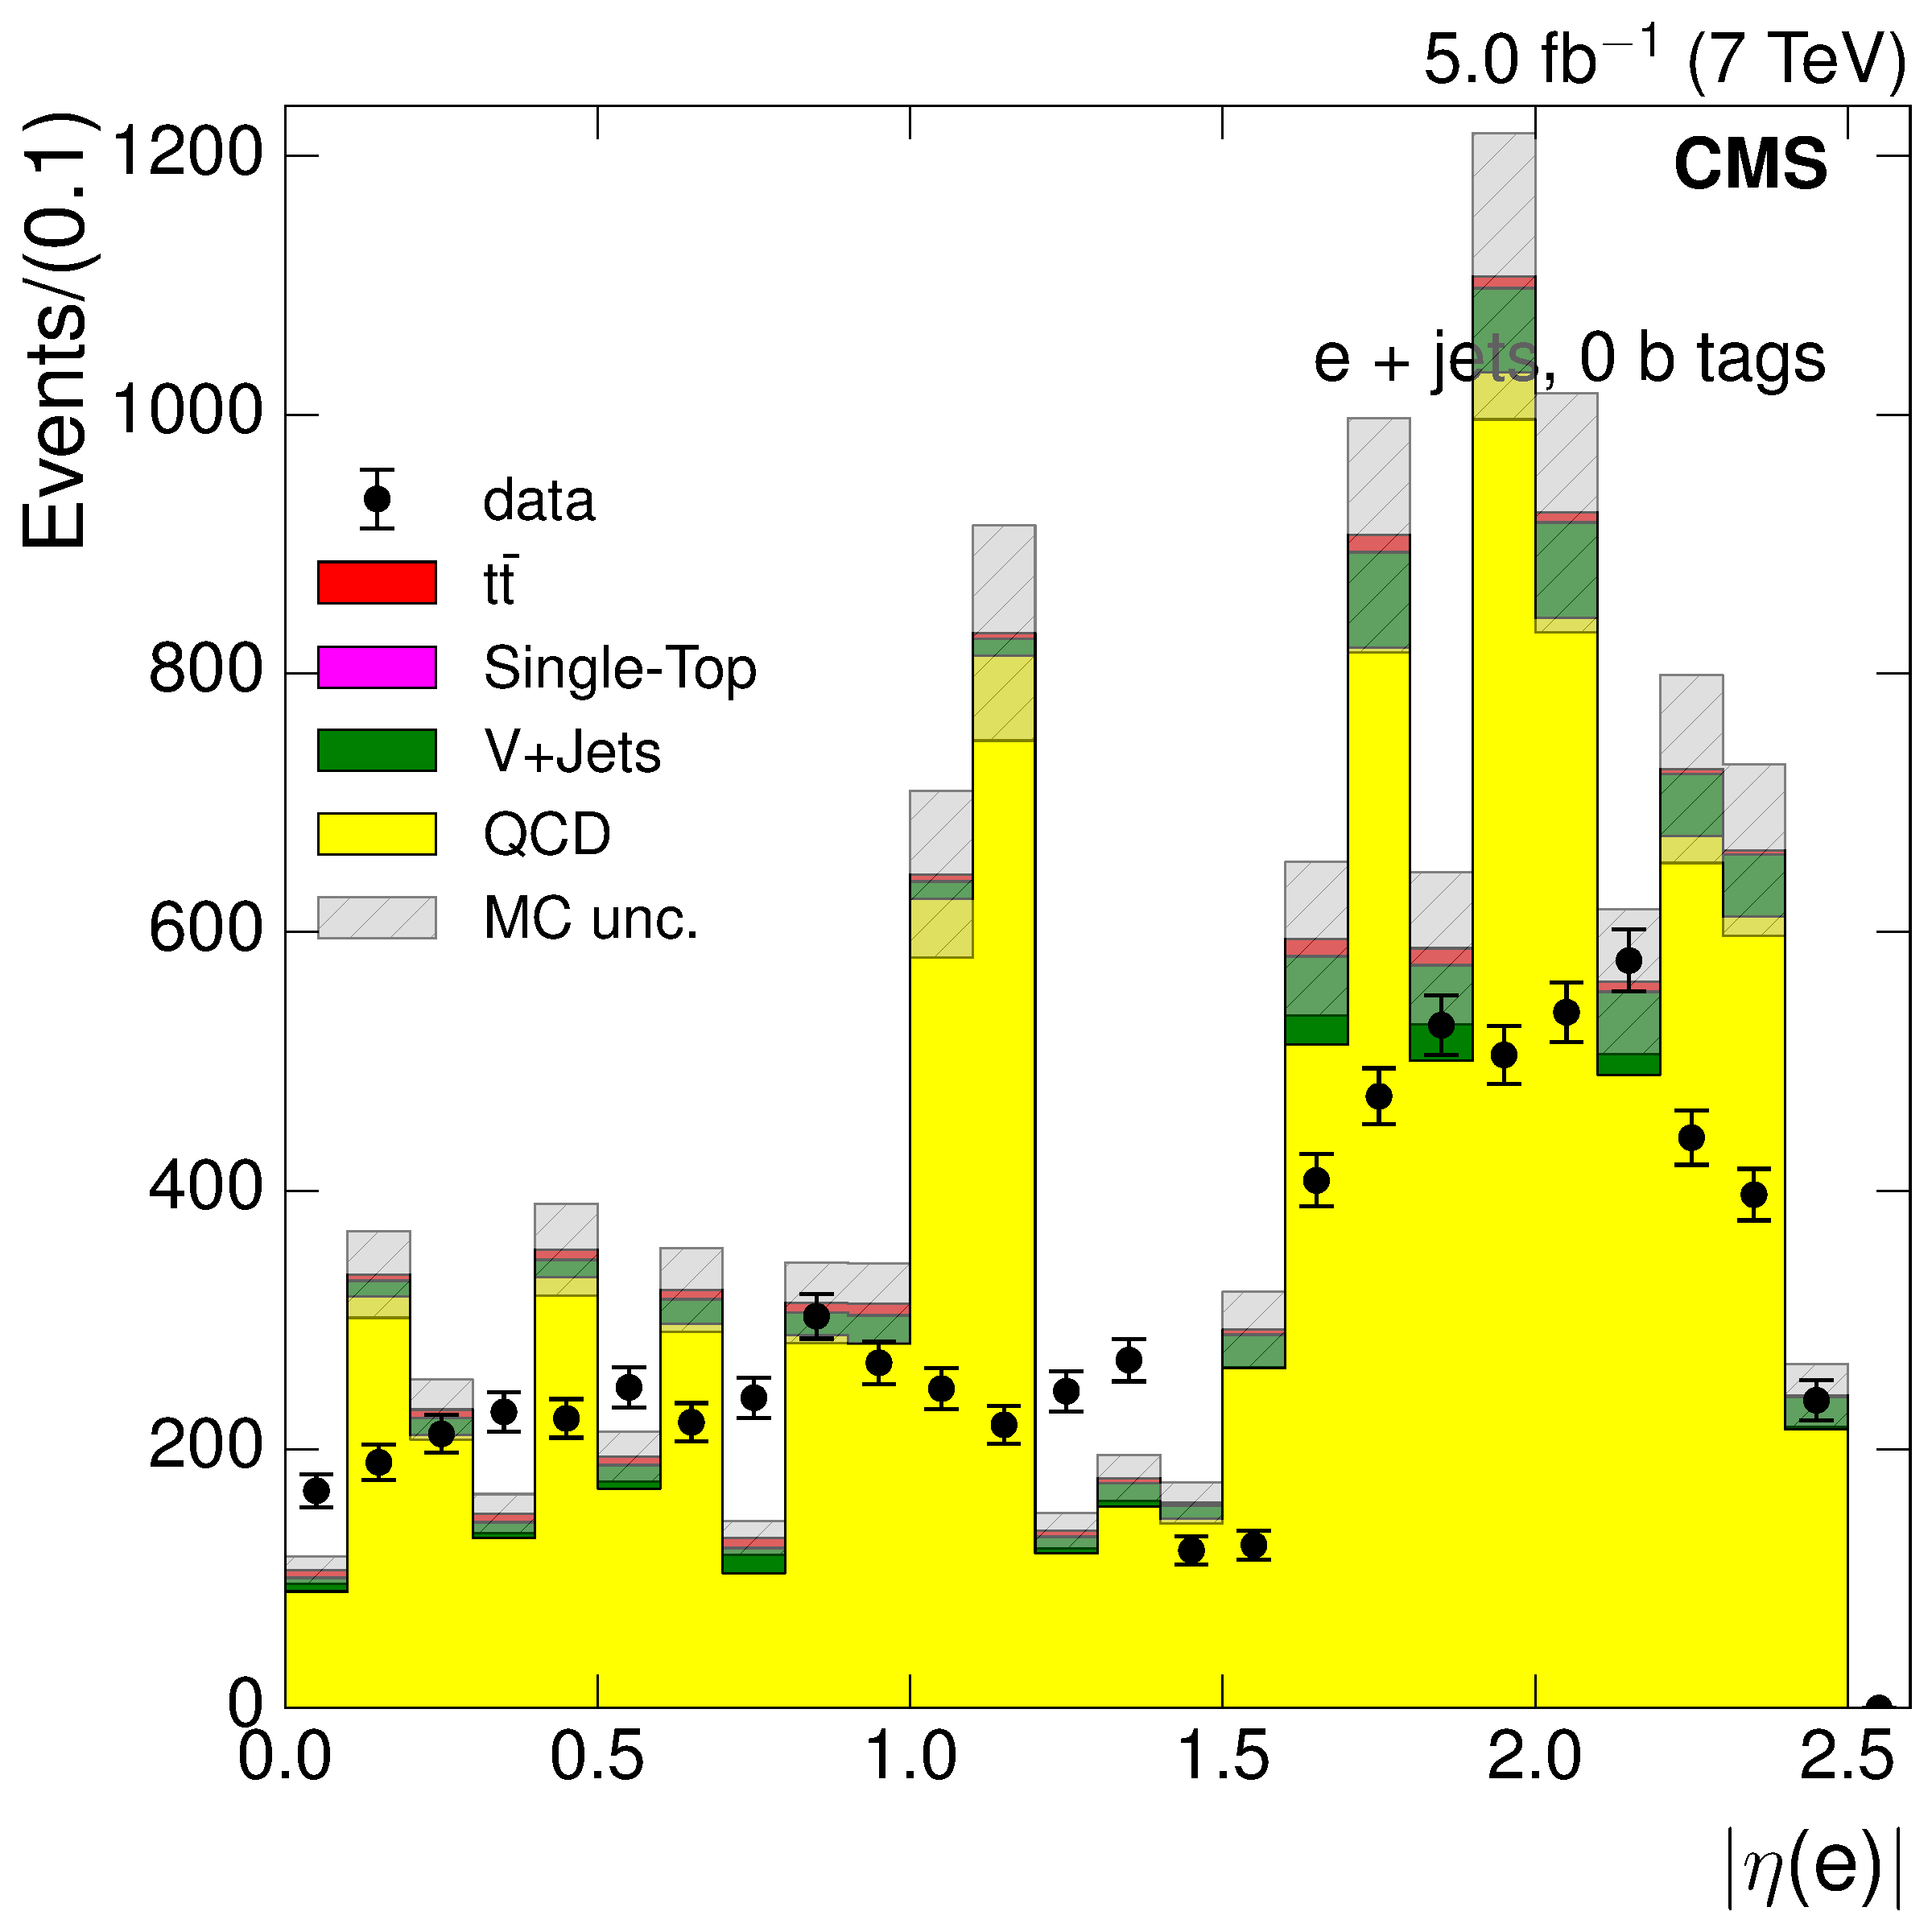
\includegraphics[width=0.45\textwidth]{Chapters/07_08_09_Analysis/Images/control_plots/before_fit/7TeV/qcd_plots/QCD_electron_AbsEta_conversion_control_region_0btag}\hfill
    	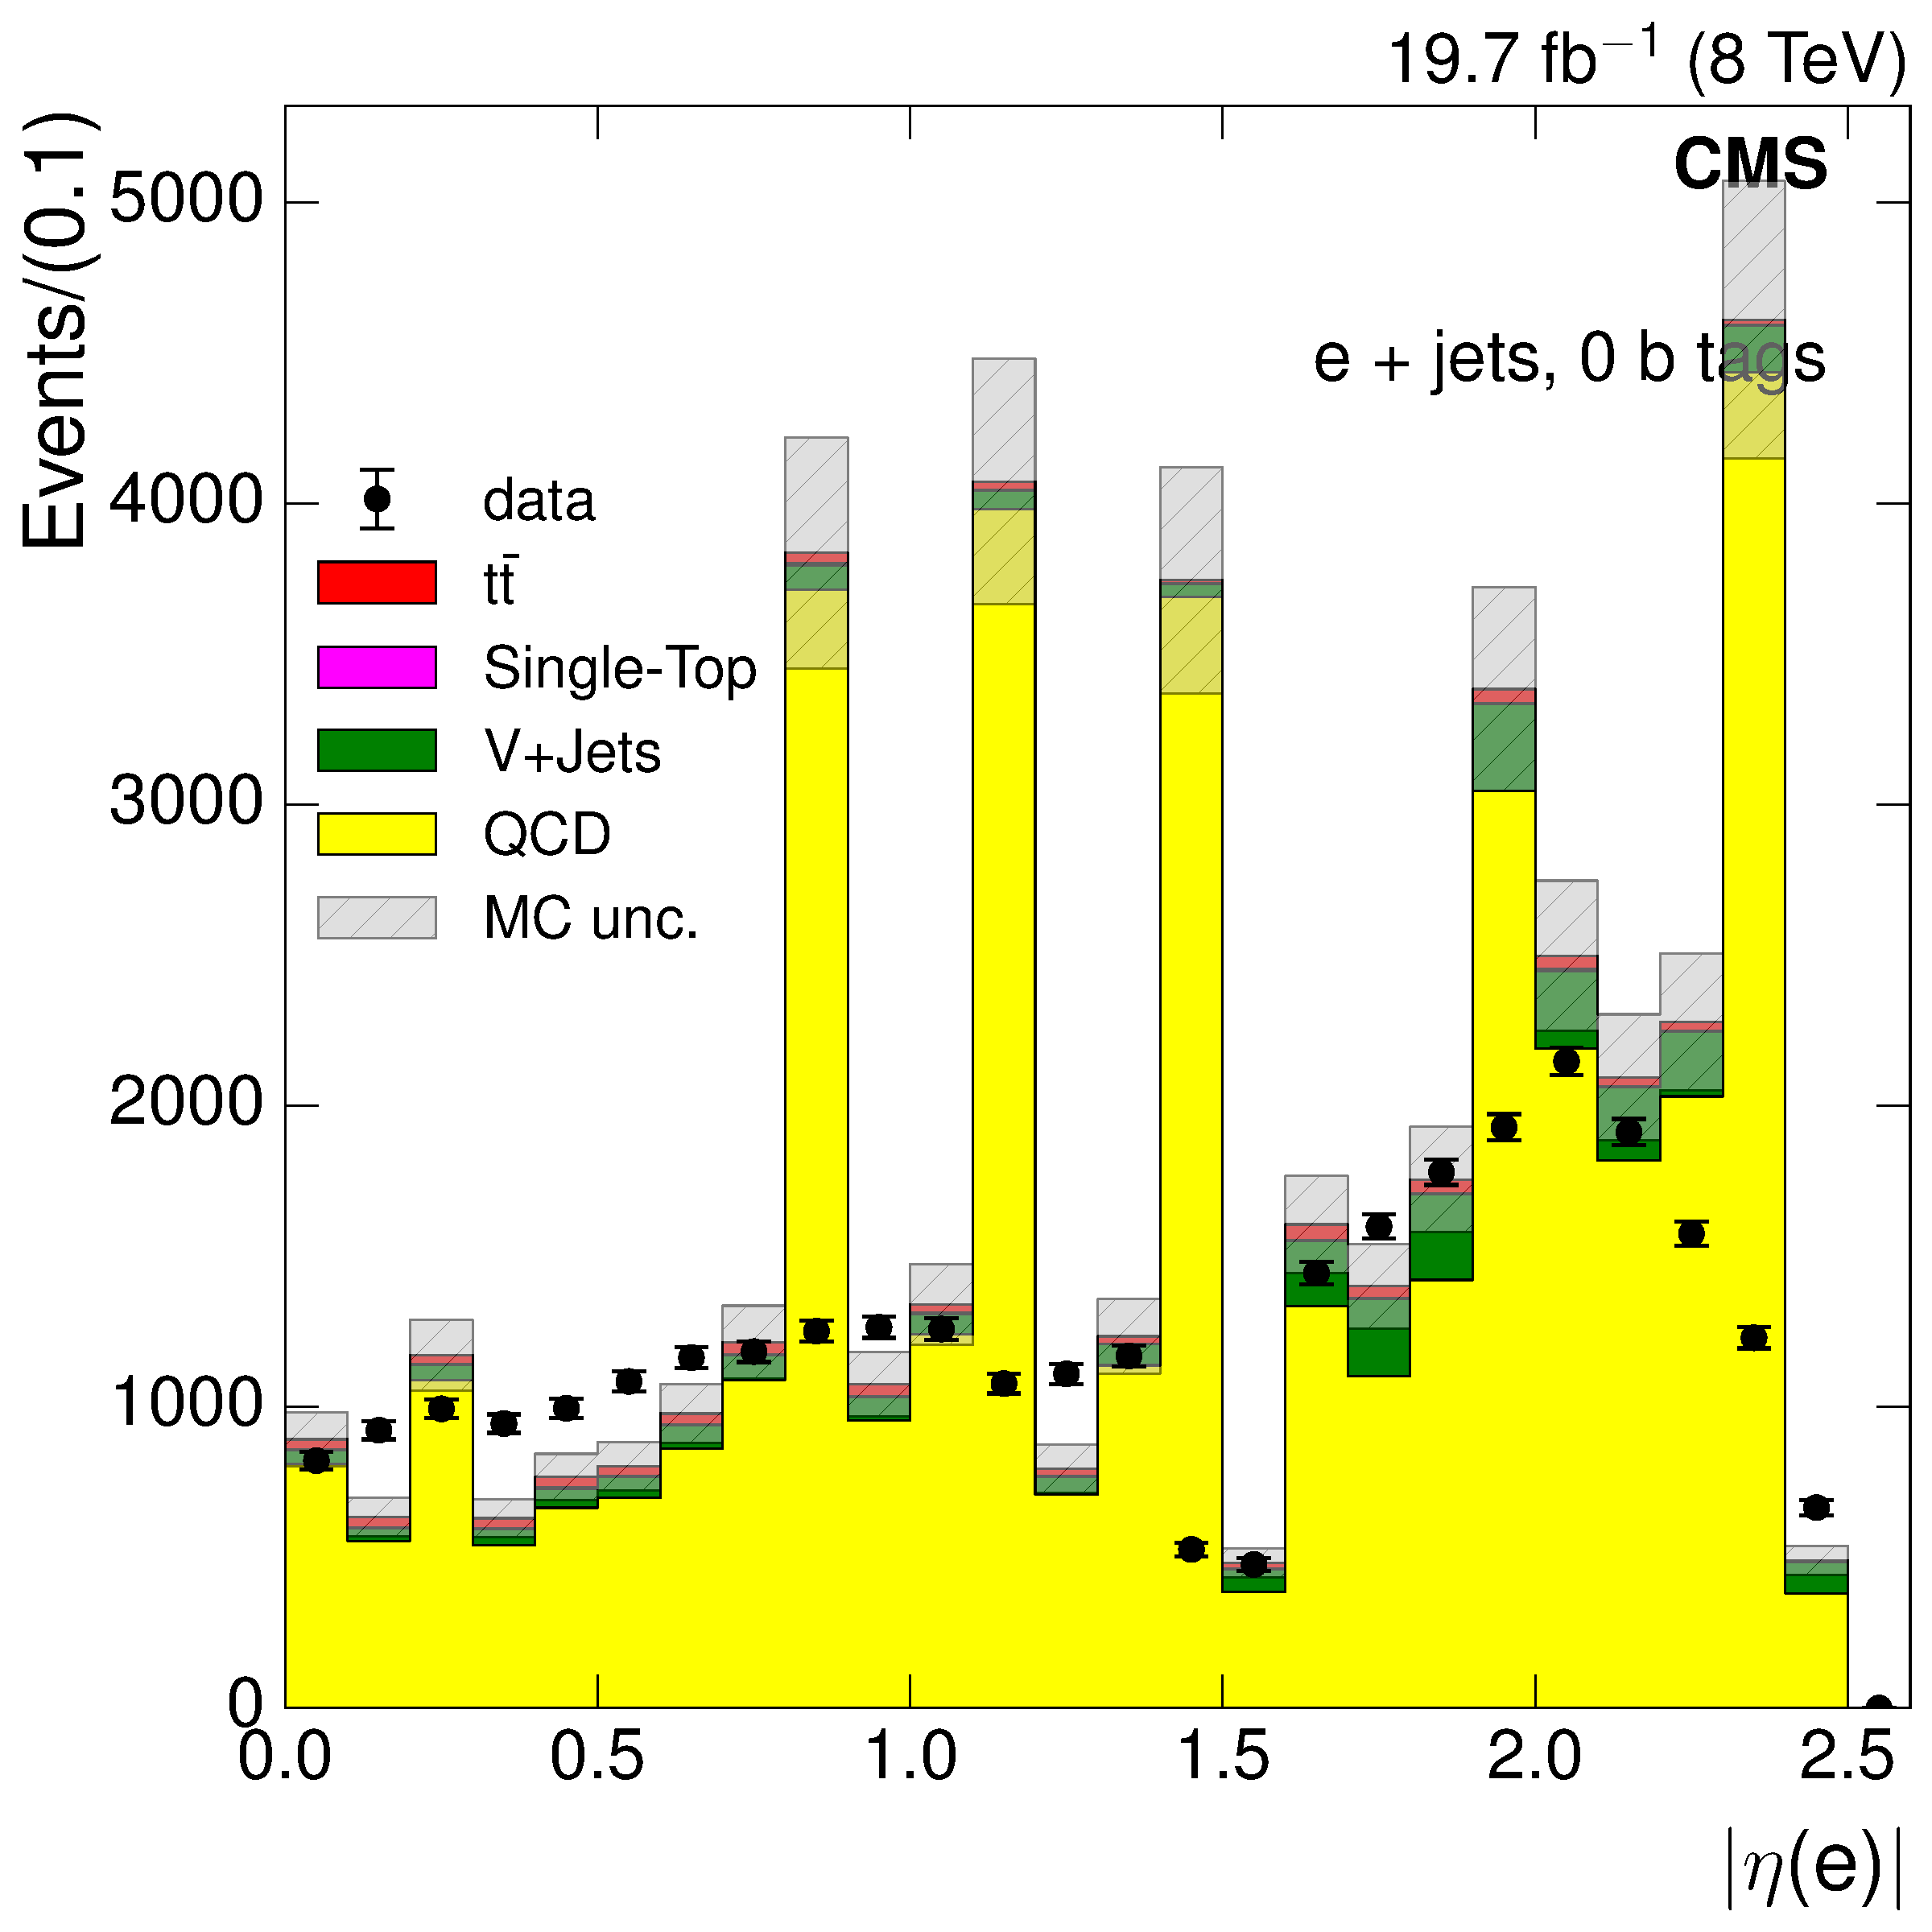
\includegraphics[width=0.45\textwidth]{Chapters/07_08_09_Analysis/Images/control_plots/before_fit/8TeV/qcd_plots/QCD_electron_AbsEta_conversion_control_region_0btag}
	  	\label{subfig:qcd_conversion_region}
	}\\
  	\subfloat[]{
  		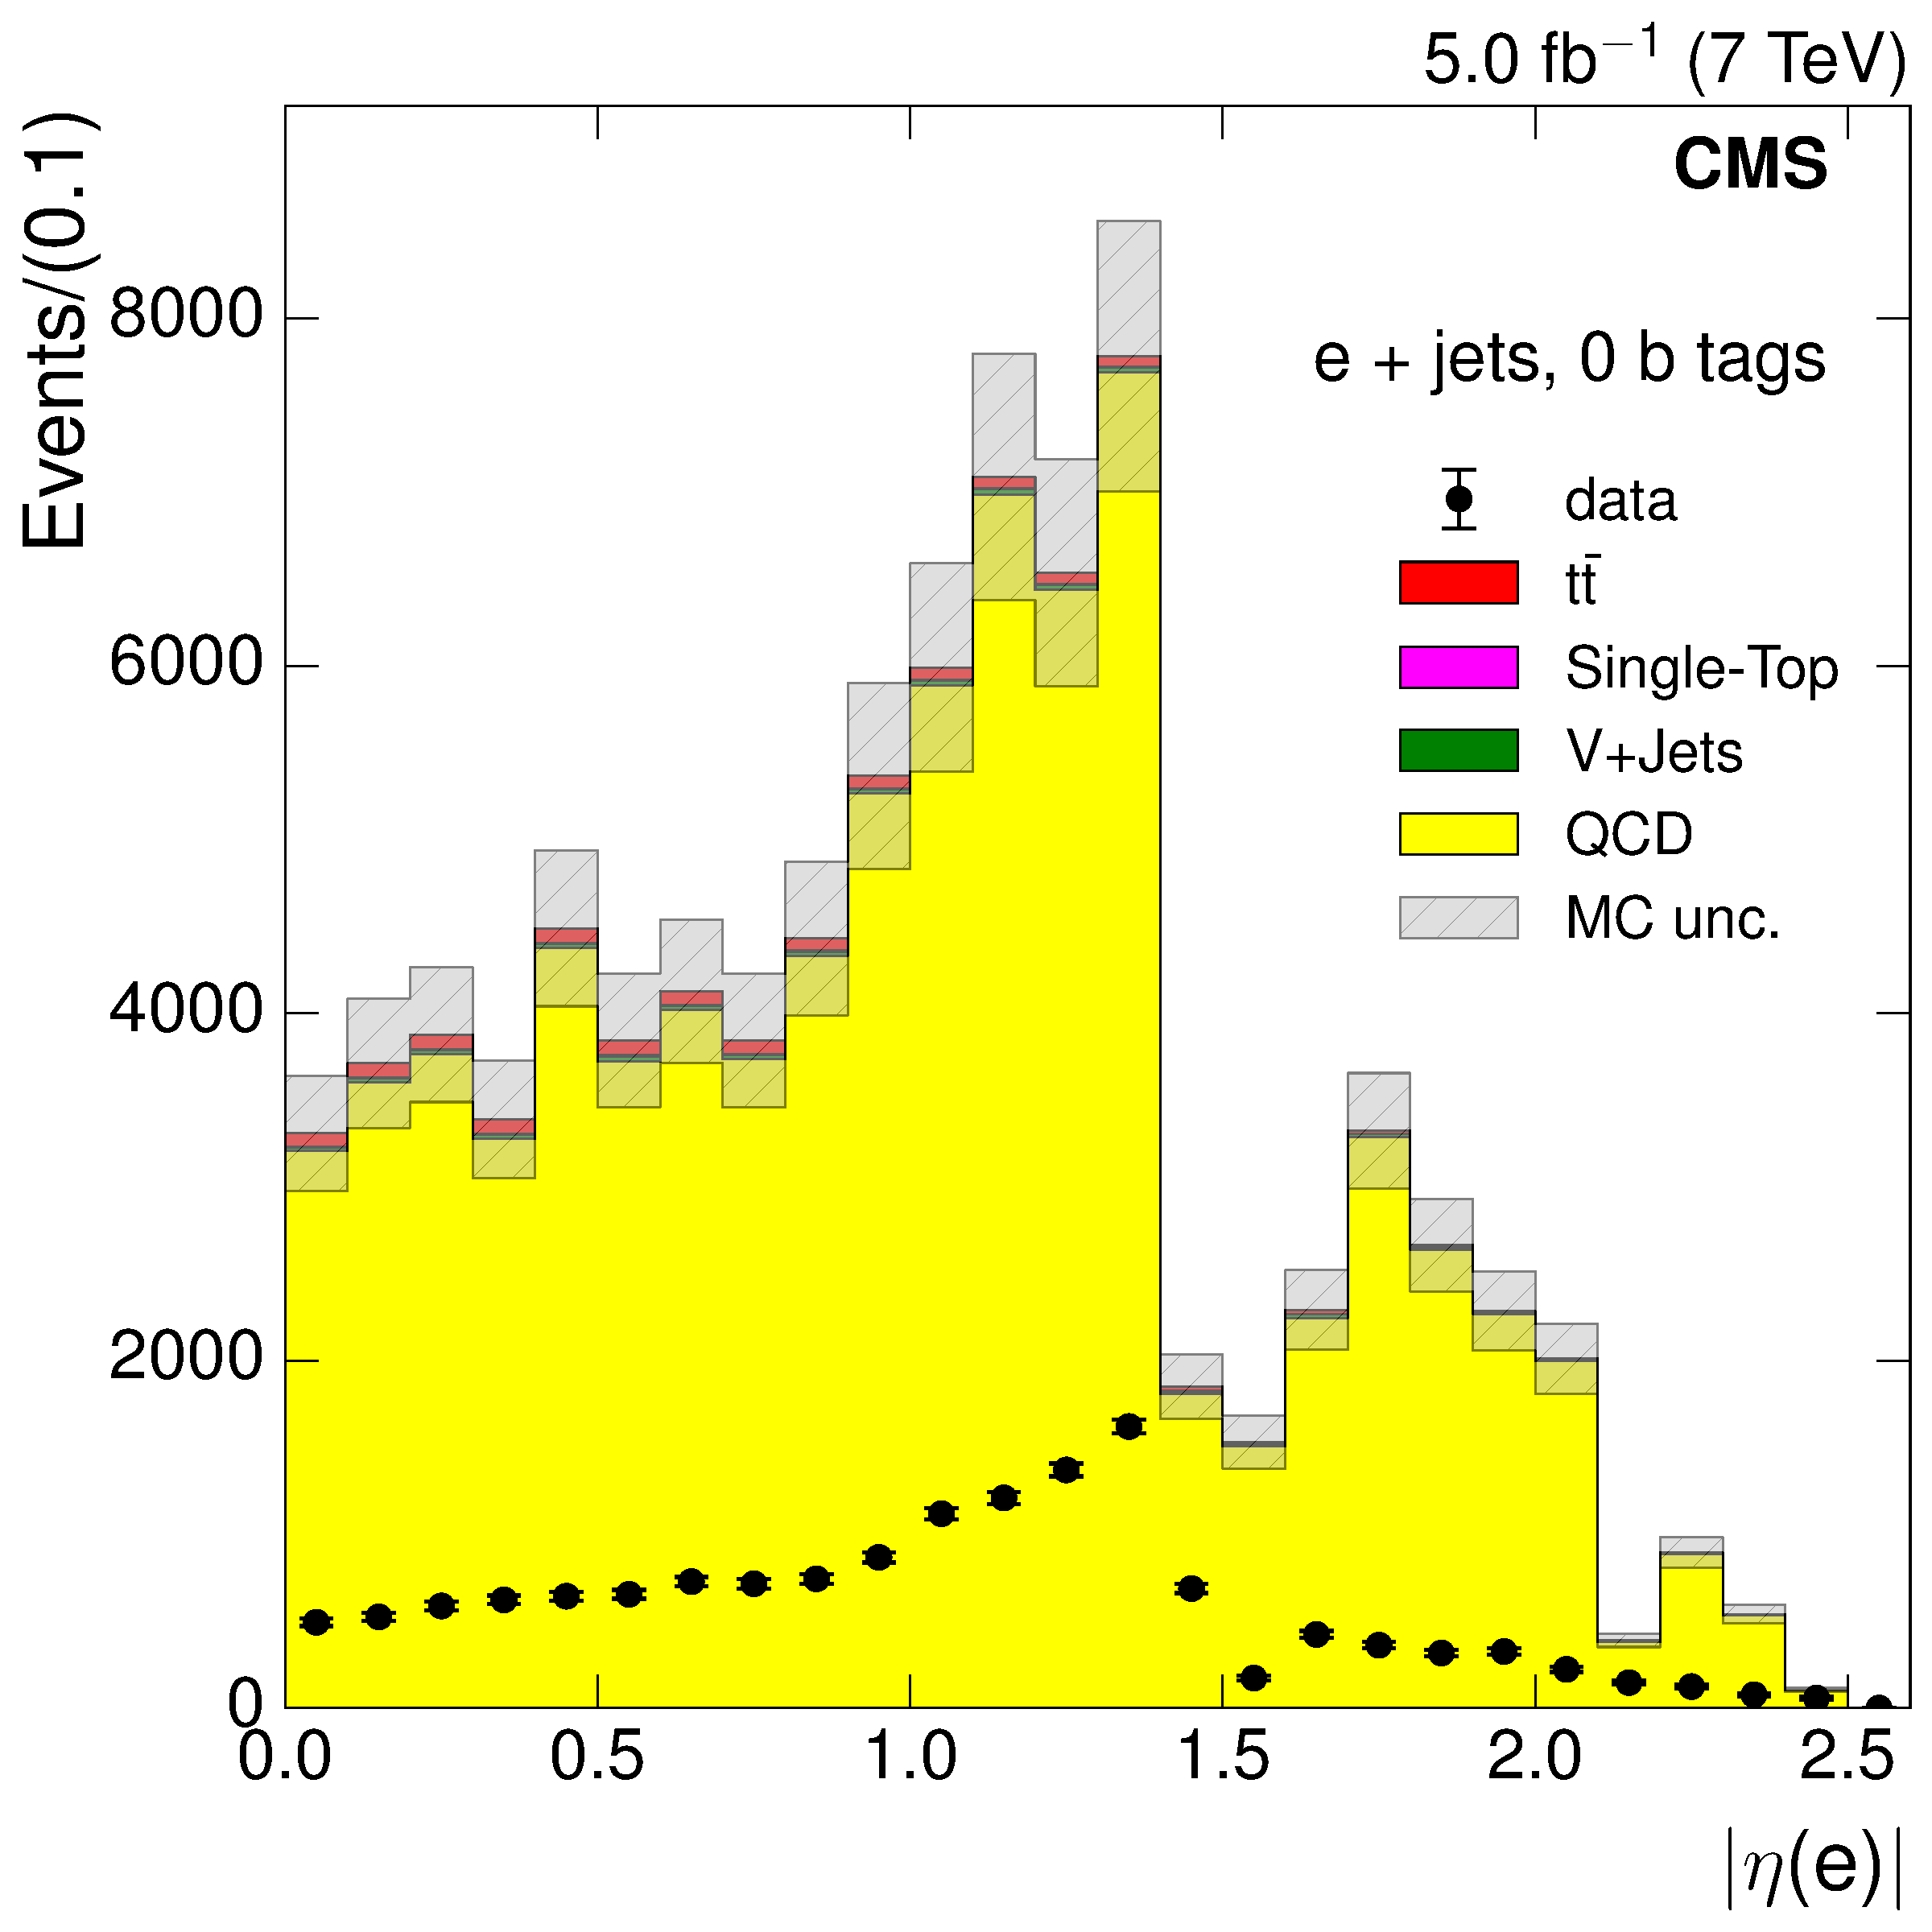
\includegraphics[width=0.45\textwidth]{Chapters/07_08_09_Analysis/Images/control_plots/before_fit/7TeV/qcd_plots/QCD_electron_AbsEta_non_iso_control_region_0btag}\hfill
	  	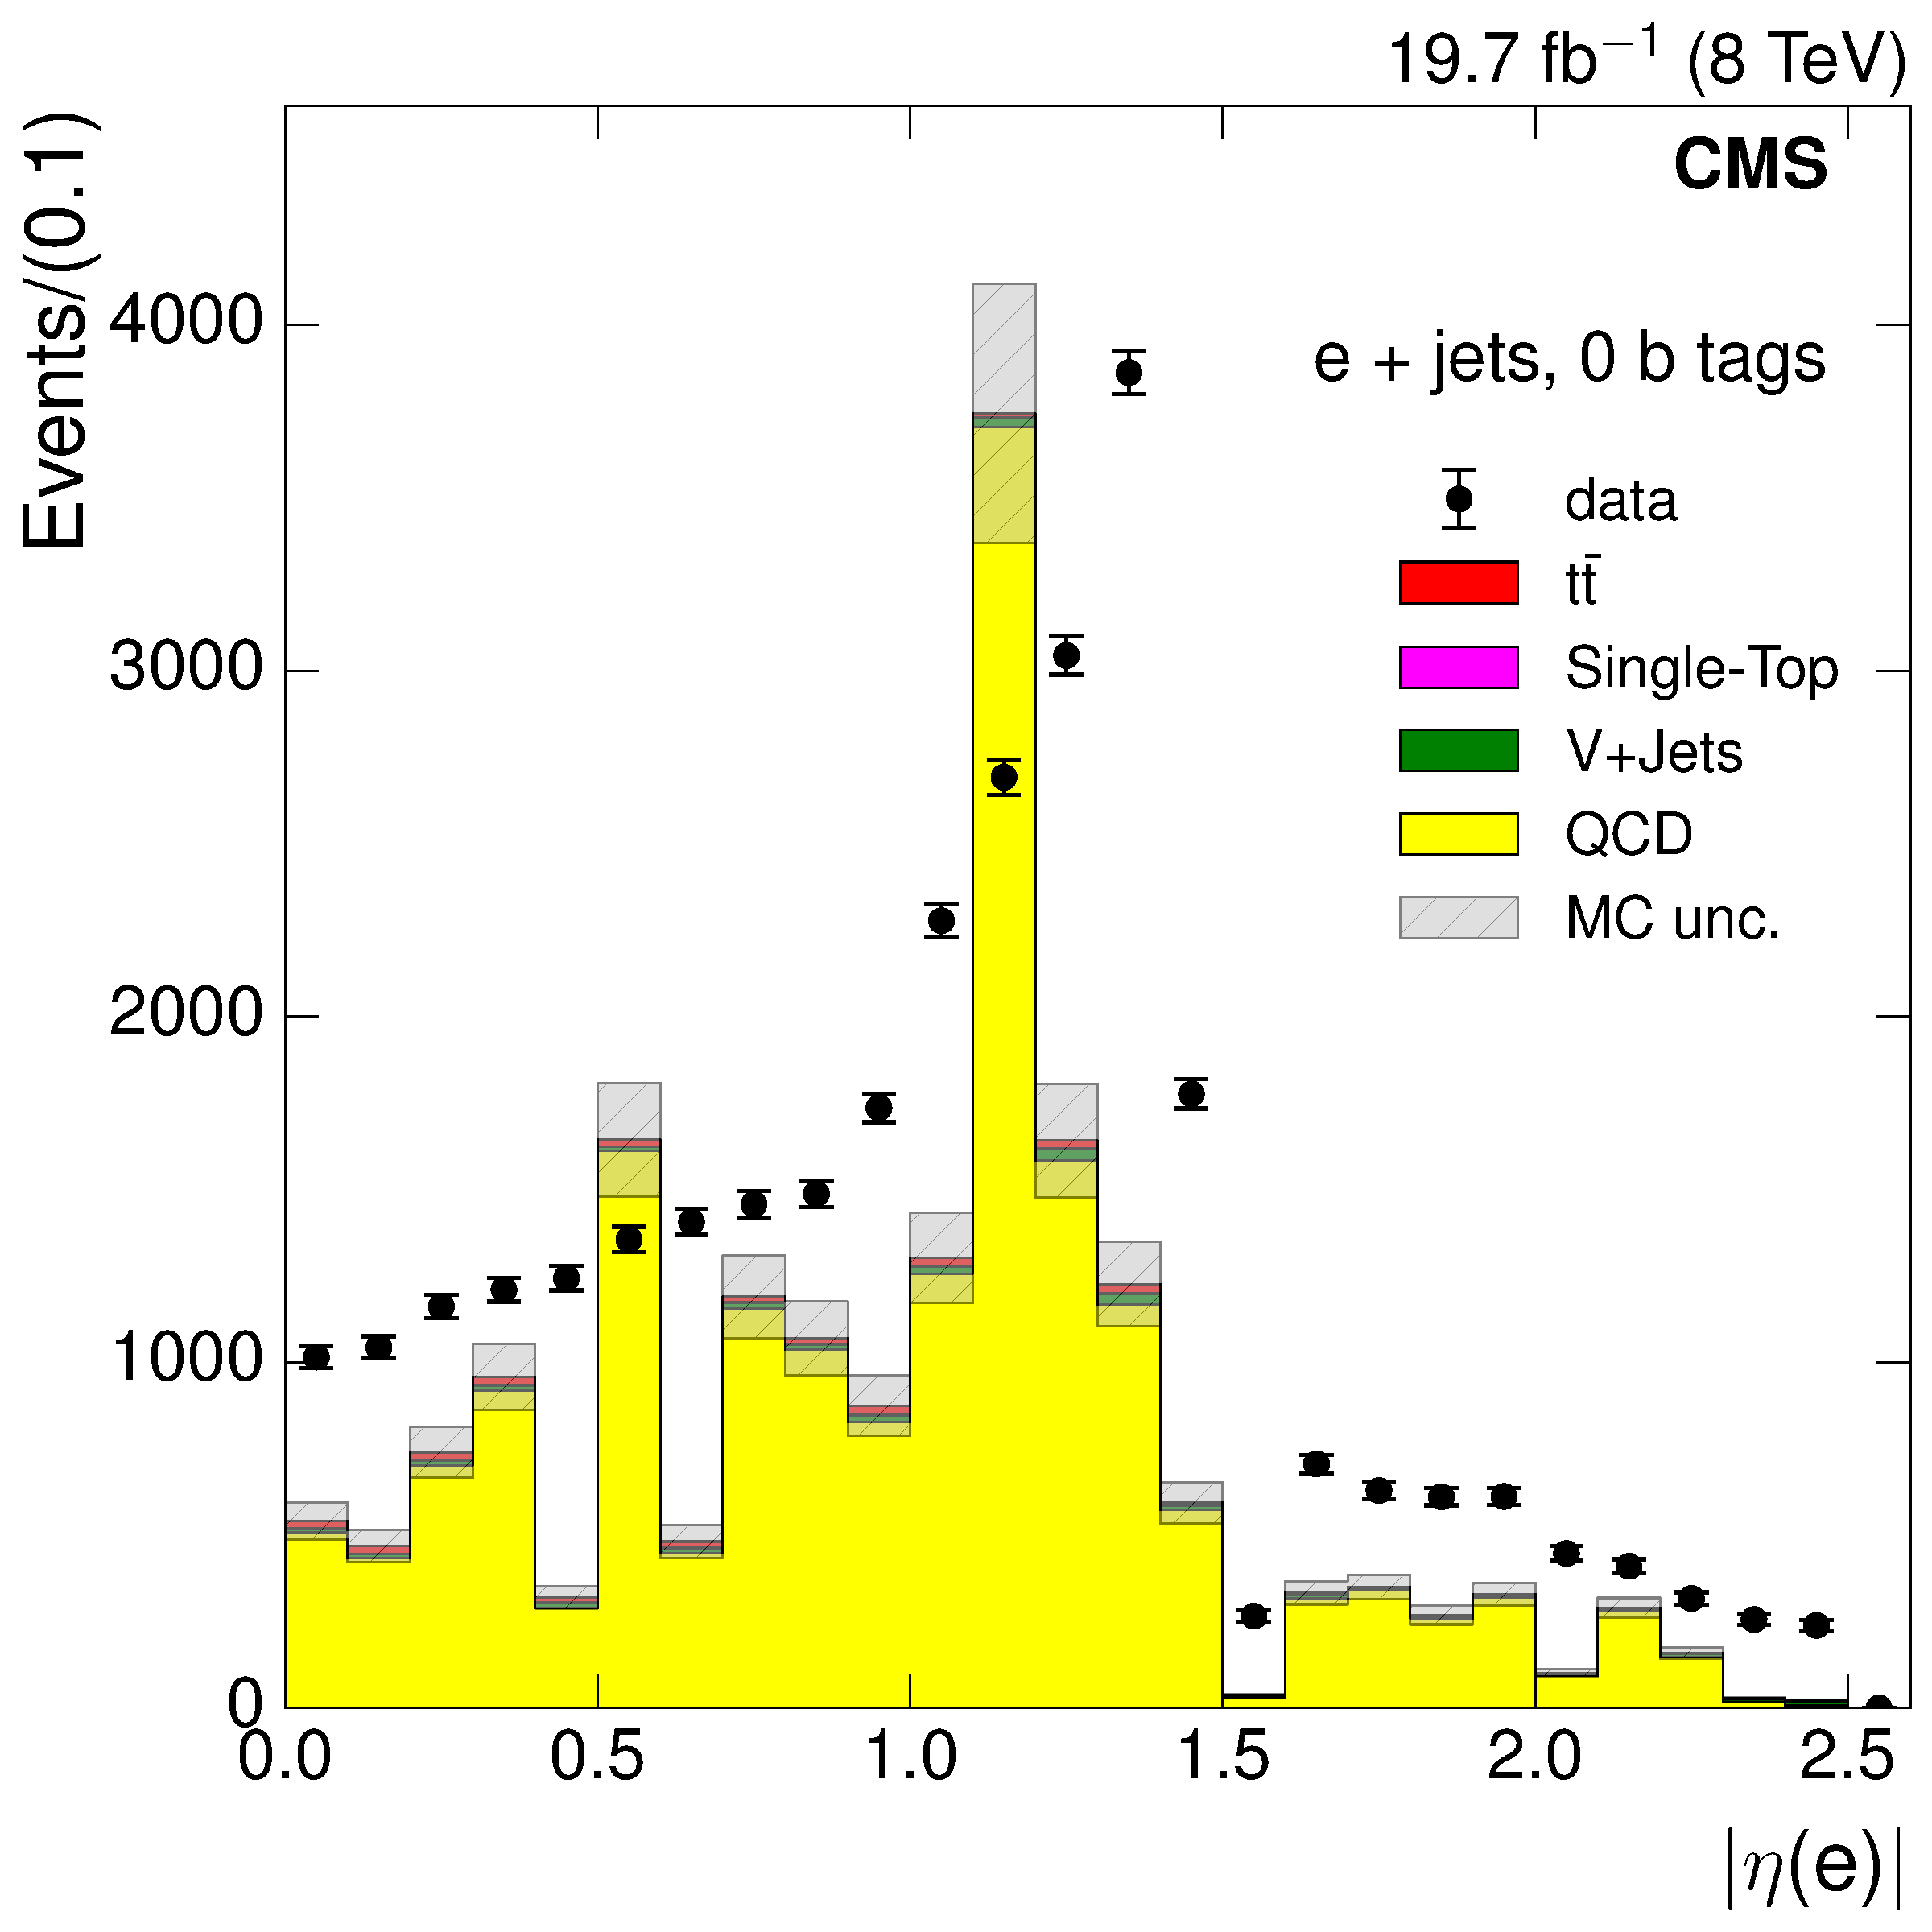
\includegraphics[width=0.45\textwidth]{Chapters/07_08_09_Analysis/Images/control_plots/before_fit/8TeV/qcd_plots/QCD_electron_AbsEta_non_iso_control_region_0btag}
	  	\label{subfig:non-isolated_region}
	}\\
  	\subfloat[]{
  		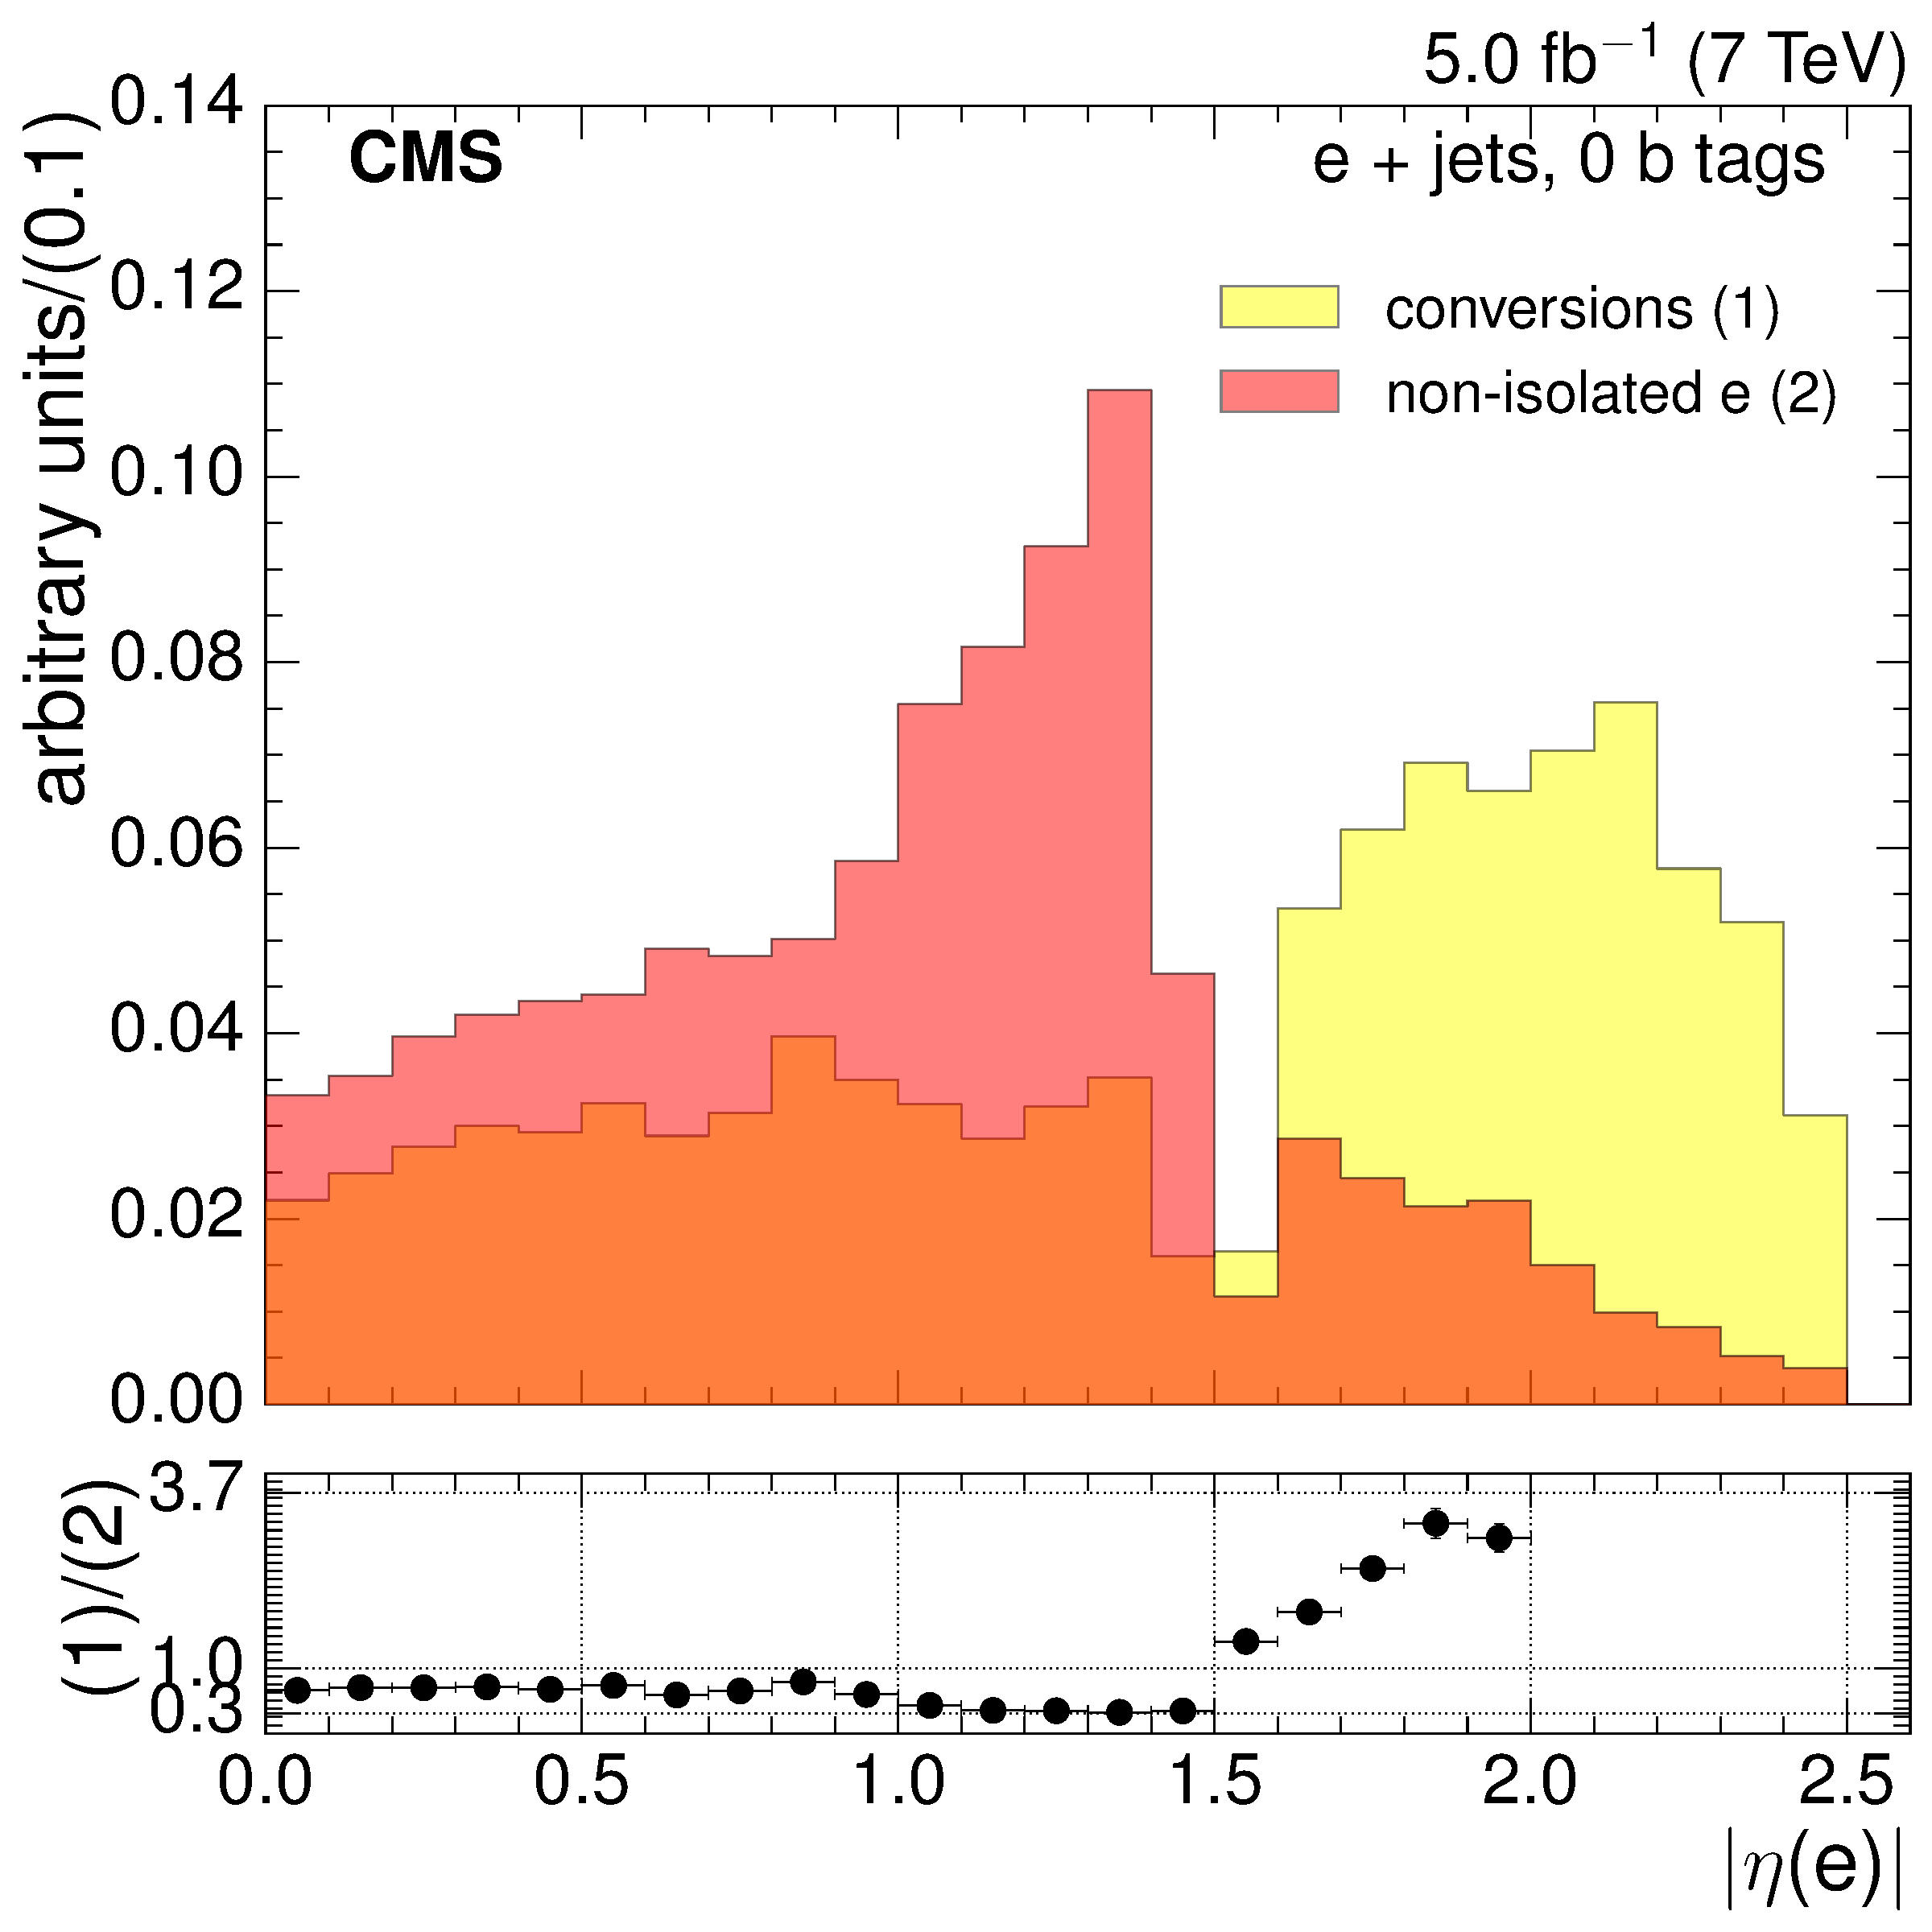
\includegraphics[width=0.45\textwidth]{Chapters/07_08_09_Analysis/Images/control_plots/before_fit/7TeV/qcd_plots/shape_comparisons/QCD_electron_AbsEta_control_region_comparison_0btag}\hfill
	  	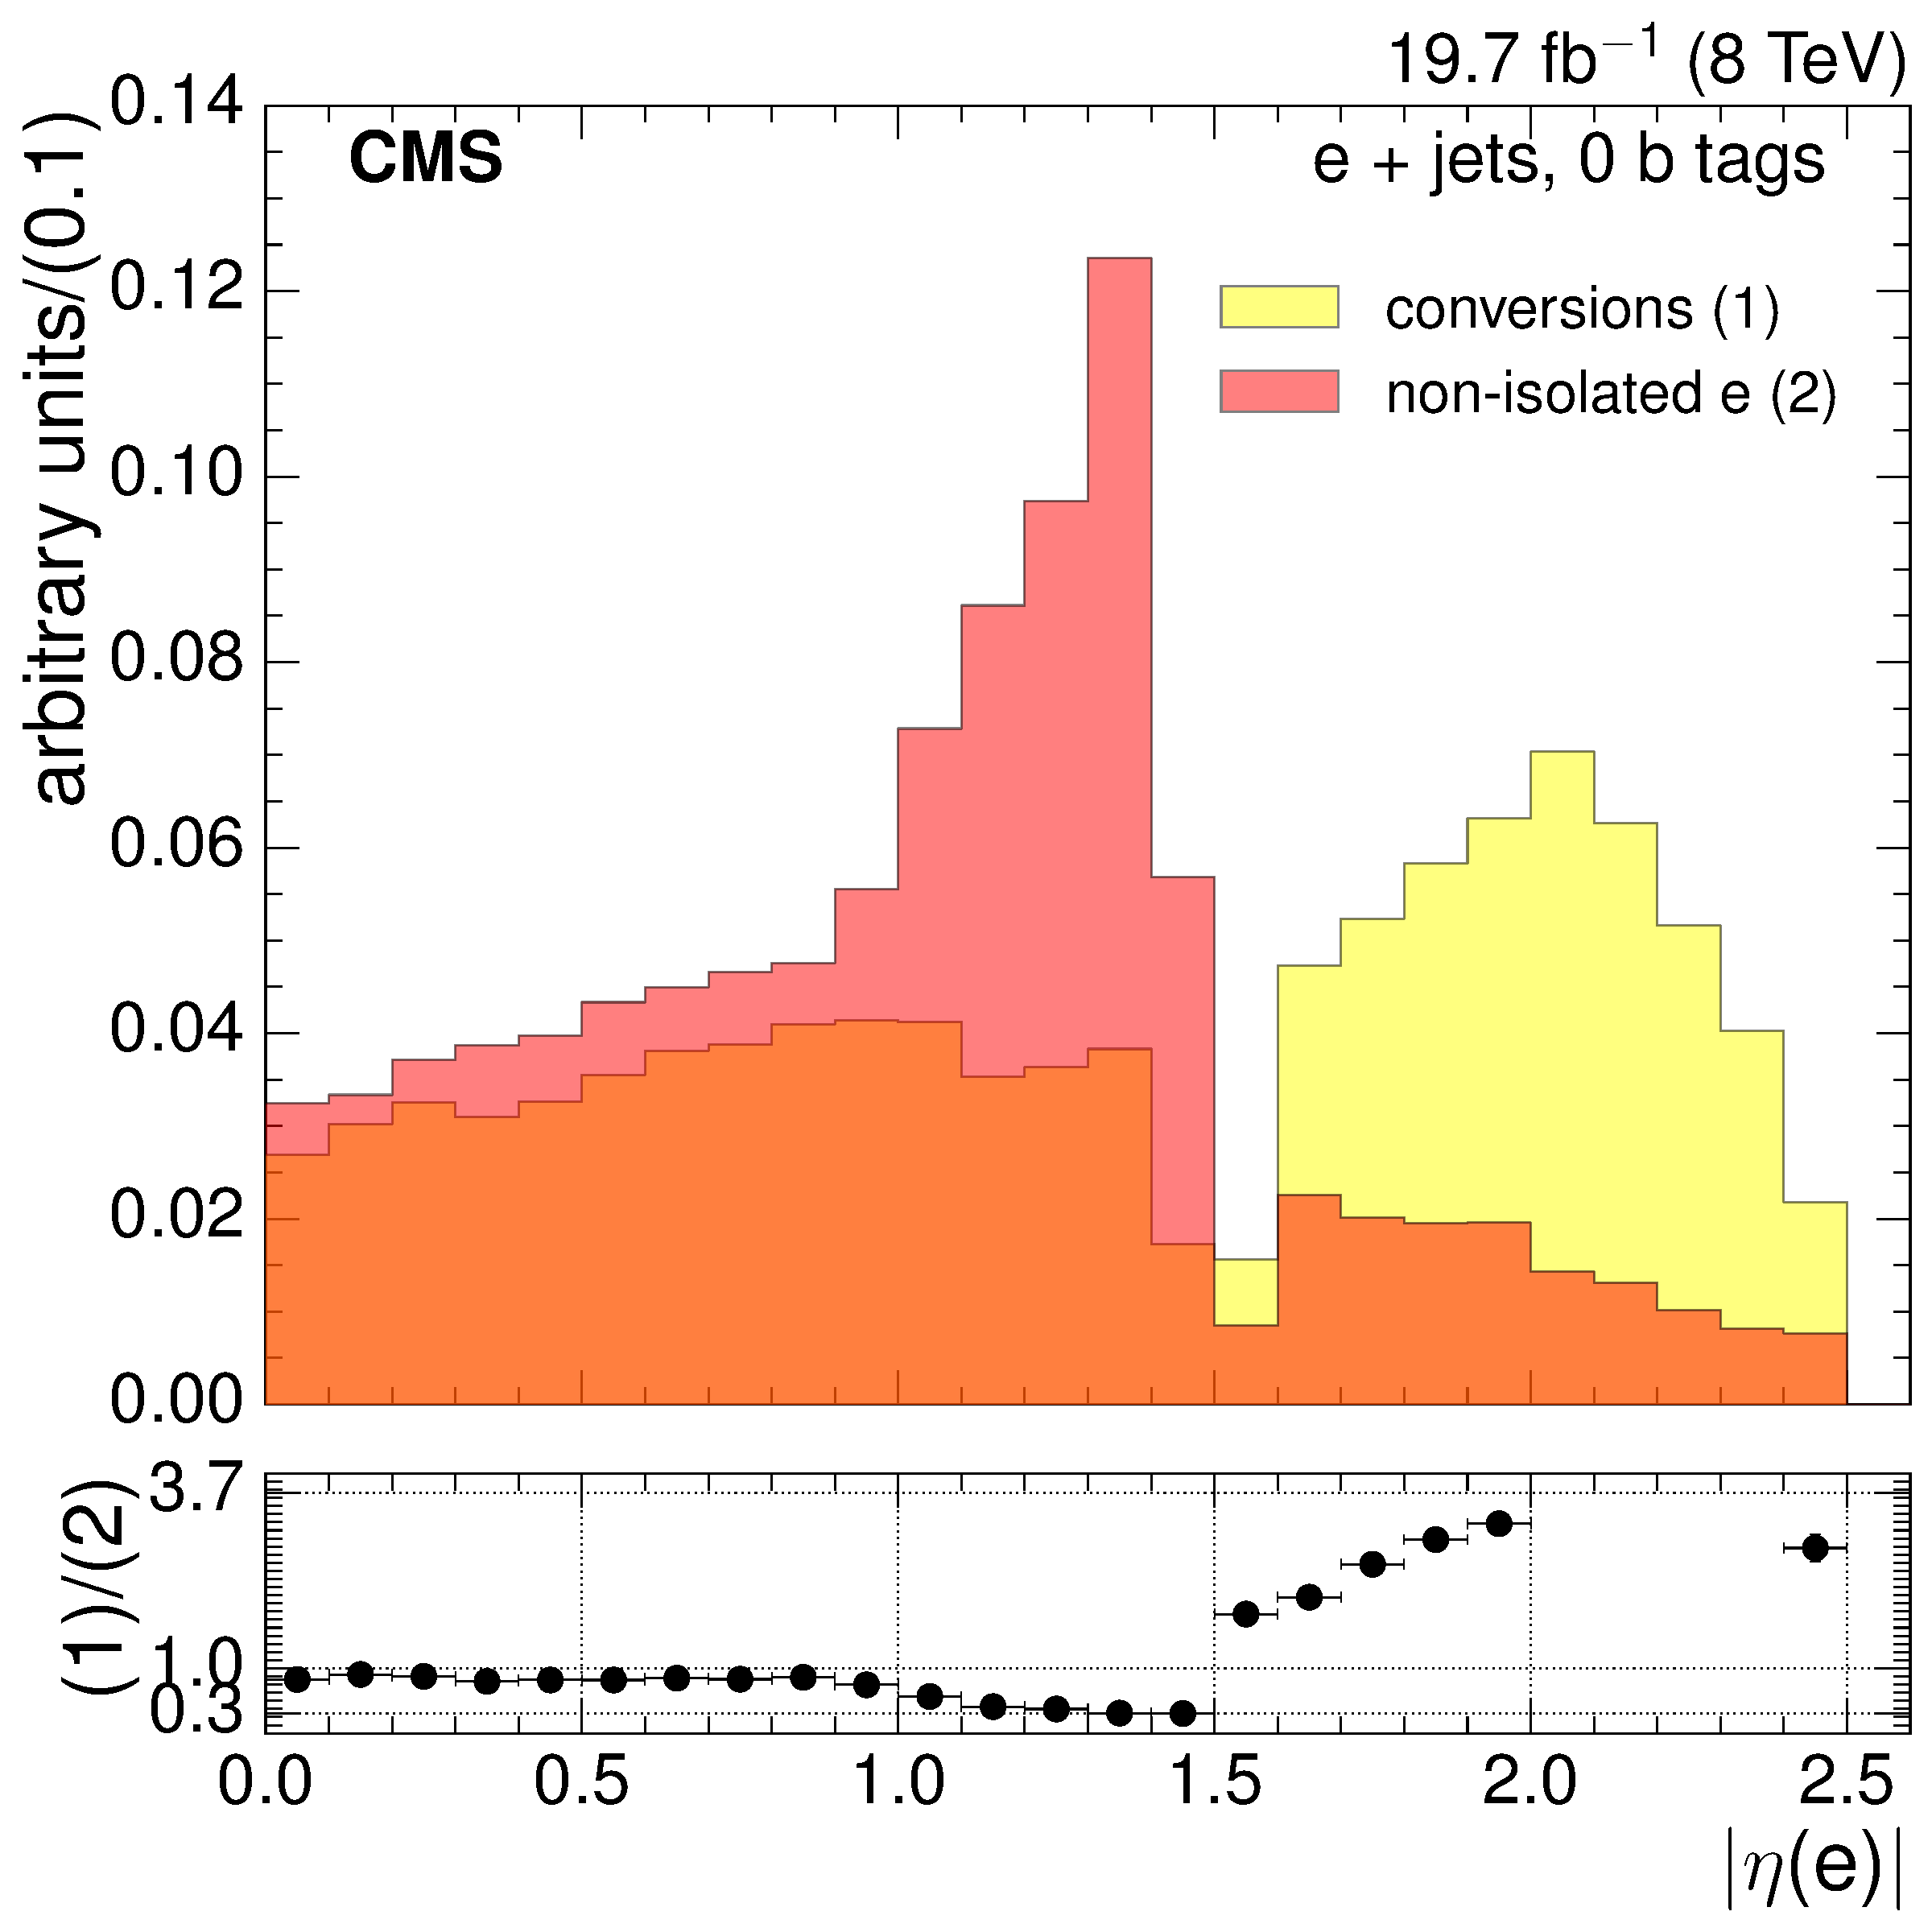
\includegraphics[width=0.45\textwidth]{Chapters/07_08_09_Analysis/Images/control_plots/before_fit/8TeV/qcd_plots/shape_comparisons/QCD_electron_AbsEta_control_region_comparison_0btag}
	  	\label{subfig:control_region_comparison}
	}\\
  	\caption[Comparison of QCD selections in the electron+jets channel at $\roots=7\TeV$ and at
    $\roots=8\TeV$.]{Electron \abseta distributions in QCD selections in the electron+jets channel at
    $\roots=7\TeV$ on the left and at $\roots=8\TeV$ on the right, in the conversion region (a) and in the
    non-isolated region (b). A shape comparison between the two regions in data is shown in (c).}
    \label{fig:electron_QCD}
\end{figure}

In the case of the muon+jets channel, the full selection is applied with the exception of the muon relative
isolation requirement, which is switched from $<0.12$ to $>0.3$. This cut value is chosen in order to largely
remove most background processes and produce a high purity QCD sample, as can be seen from
Figure~\ref{fig:muon_qcd_isolation}. There is a resonable agreement between MC and data here, although again
there are some spikes representing the lack of simluation statistics. As in the electron channel, the \btag
requirement is reduced to 0 \btags and in addition the jet multiplicity requirement is reduced to require at
least three jets, to improve statistics and to ensure a purer QCD sample.

\begin{figure}[hbtp]
    \centering
      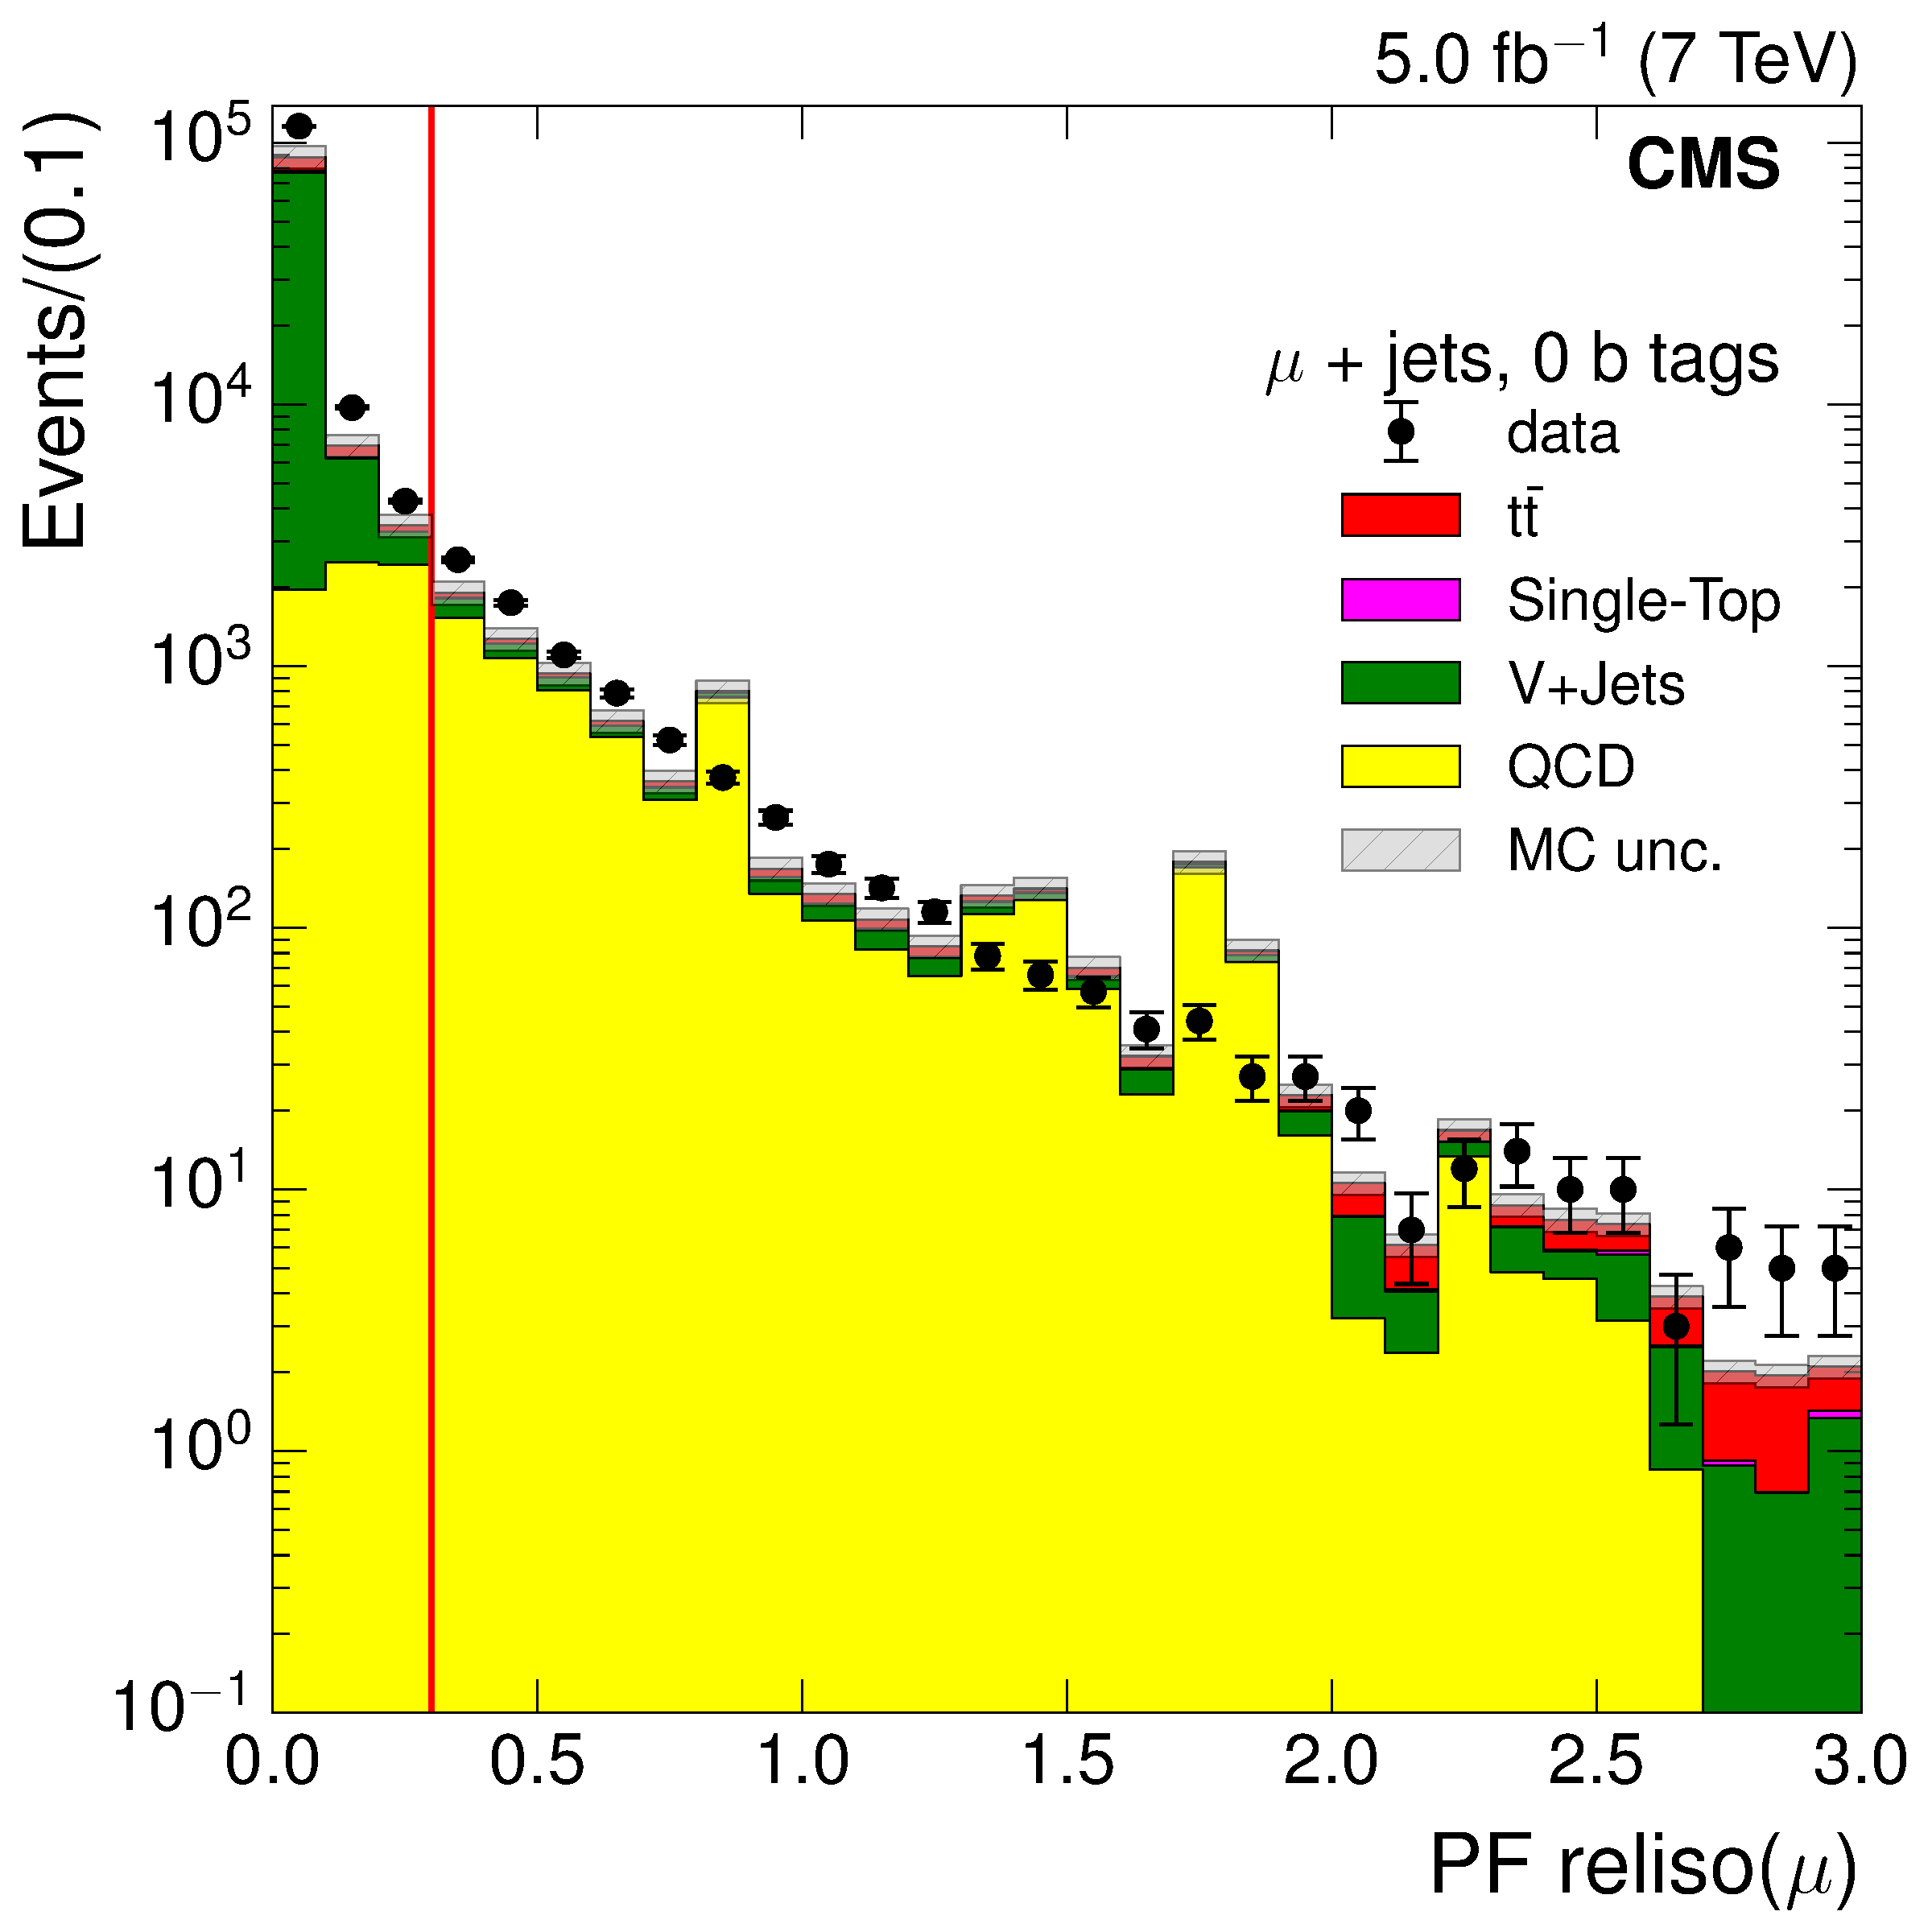
\includegraphics[width=0.48\textwidth]{Chapters/07_08_09_Analysis/Images/control_plots/before_fit/7TeV/qcd_plots/QCD_muon_pfIsolation_with_cutline_0btag}\hfill
      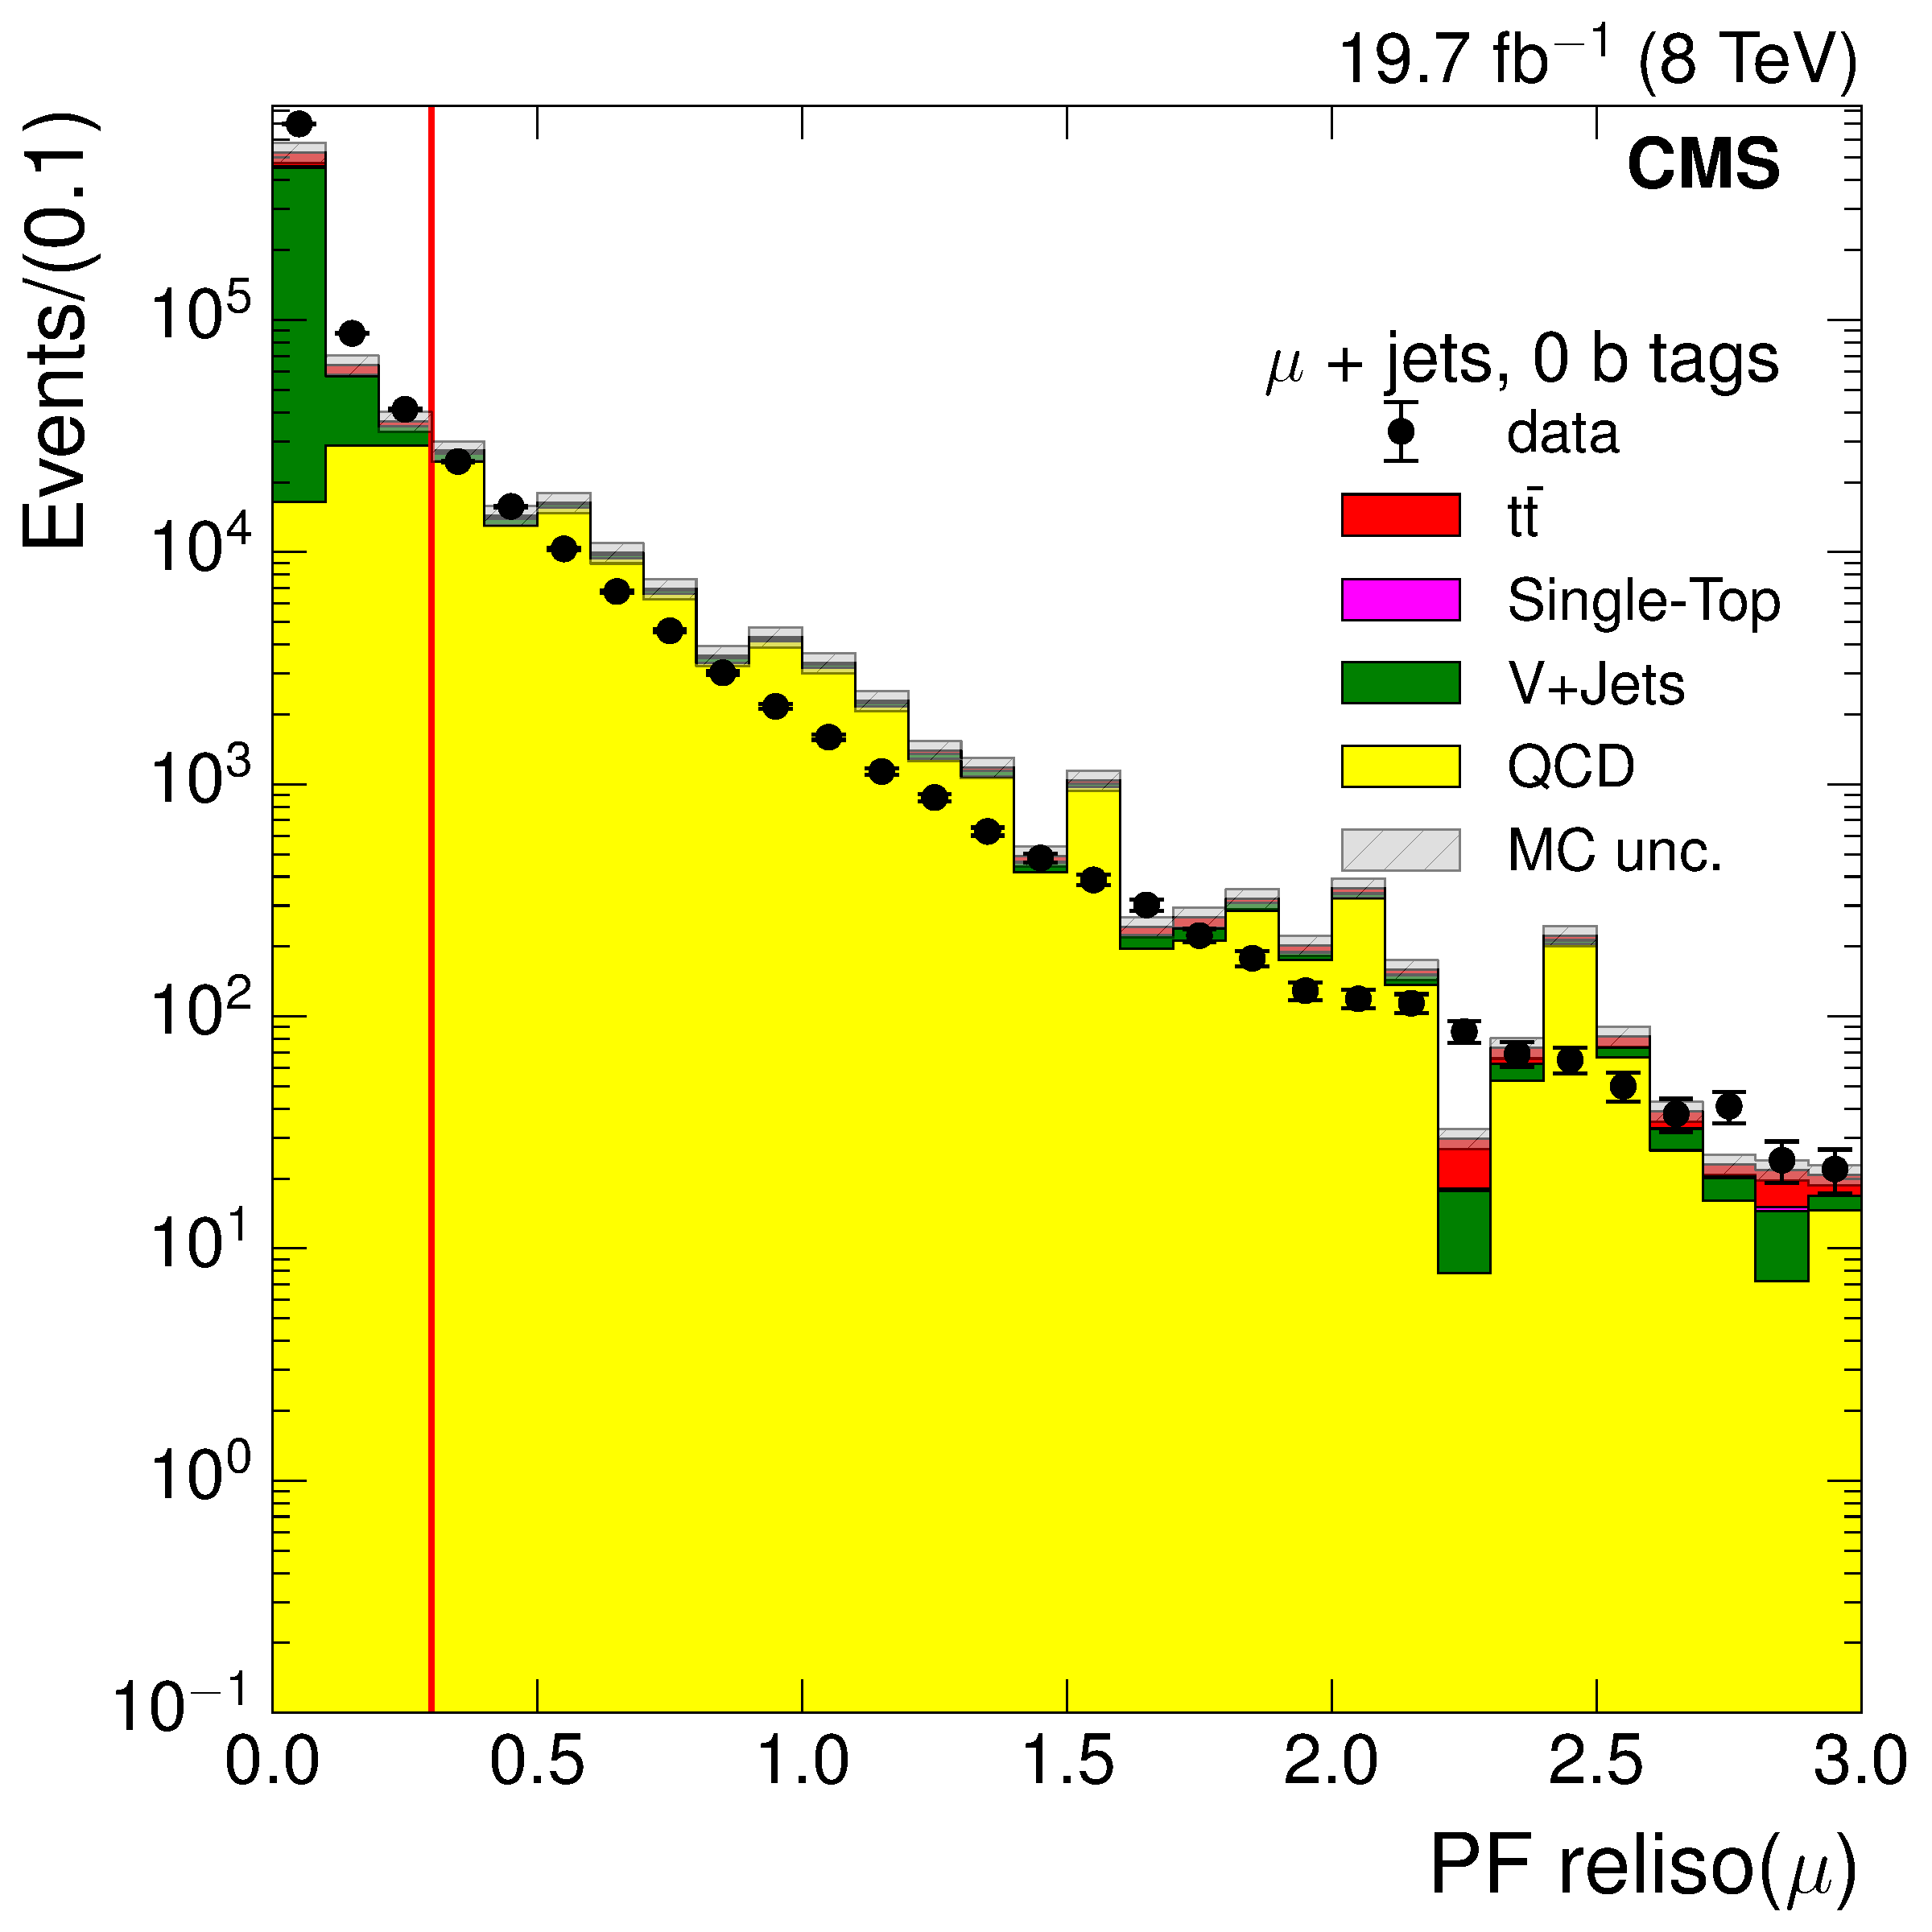
\includegraphics[width=0.48\textwidth]{Chapters/07_08_09_Analysis/Images/control_plots/before_fit/8TeV/qcd_plots/QCD_muon_pfIsolation_with_cutline_0btag}\\
      \caption[PF relative isolation distributions in the muon+jets channel at $\roots=7\TeV$ and
      $\roots=8\TeV$]{PF relative isolation distributions in the muon+jets channel, before subtraction of
      \ttbar, single top and \VpJets at $\roots=7\TeV$ (left) and $\roots=8\TeV$ (right).}
     \label{fig:muon_qcd_isolation}
\end{figure}

Relative to other processes, QCD events are computationally extremely expensive to produce in simulation,
owing to their large cross section requiring high numbers of events. Neverthless, the number of events passing
the selection will be very small compared to the number of events passing the signal selection, even with
simulated samples with high statistics, meaning there is limited value in obtaining additional statistics
for QCD samples. Since the number of events passing the QCD background selections is relatively low, the
effect of even large uncertainties in the QCD background on the total number of events will be minimal.

Due to the low statistics of the QCD samples obtained from data, the inclusive QCD shape over all bins is used
in every bin for each primary variable (meaning the shape is obtained over the full range of the primary
variables, rather splitting into bins). The remaining contribution from \ttbar, single-top and \W/\ZpJets
processes is subtracted from the data sample using the estimation from Monte Carlo simulation. The resulting
template of QCD events from data is then used later in the fitting procedure, in place of the equivalent Monte
Carlo template (Section~\ref{ss:data-mc_comparison}).

\section{Data-MC scale factors}
\label{s:data_mc_scale_factors}
The following sections describe the small but significant discrepancies that exist between data and simulation
regarding pileup modelling~\ref{ss:pileup}; \btagging~\ref{ss:b_tagging}; trigger, identification and
isolation efficiency~\ref{ss:trigger_ID_isolation_corrections}; jet energy scale and jet energy
resolution~\ref{sss:jet_energy_scale}; and \met calculation~\ref{ss:met_corrections}. Scale factors and
corrections are applied to both MC and data to account for these differences. The data-MC scale factors used
are in accordance with the CMS TOP PAG, and the relevant corrections are implemented for 7\TeV and 8\TeV.

\subsection{Pileup}
\label{ss:pileup}
Monte Carlo simulation events are produced by first creating the hard proton-proton interaction of interest in
a proton bunch crossing, and then introducing the additional interactions, pileup. The pileup distribution in
simulation does not reflect the true distribution in data, therefore pileup reweighting is carried out. The
estimation of the pileup distribution in data is obtained using the total inelastic proton-proton cross
section and the instantaneous luminosity measured in each proton bunch crossing, with a tool provided by the
CMS Physics Validation Group. For each number of pileup interactions in simulation, a weight is then produced
to match the respective distribution in data.

There is an uncertainty on the measured luminosity which is currently 2.6~\% for 2012 data~\cite{CMS:2013gfa}
and 2.2~\% for 2011 data~\cite{CMS:2012eui}. The total inelastic cross section has been reported using CMS
forward calorimetry~\cite{Chatrchyan:2012gwa} and by the TOTEM collaboration~\cite{Antchev:2011vs}. Based on
these studies, the CMS recommended central values of 68.0\mb~ for $\roots=7$ and 69.3\mb~ for $\roots=8$ have
been used, with a $\pm5~\%$ uncertainty to account for pileup and physics modelling in simulation.

The distributions of the number of reconstructed vertices before and after applying pileup reweighting in the
electron+jets channel is shown in Figure~\ref{fig:nvertices_before_and_after_pileup_reweighting_electrons},
and in the muon+jets channel is shown in Figure~\ref{fig:nvertices_before_and_after_pileup_reweighting_muons}
in Appendix~\ref{as:data_monte_carlo_corrections}. The distributions show good agreement after reweighting.

\begin{figure}[hbtp]
    \centering
      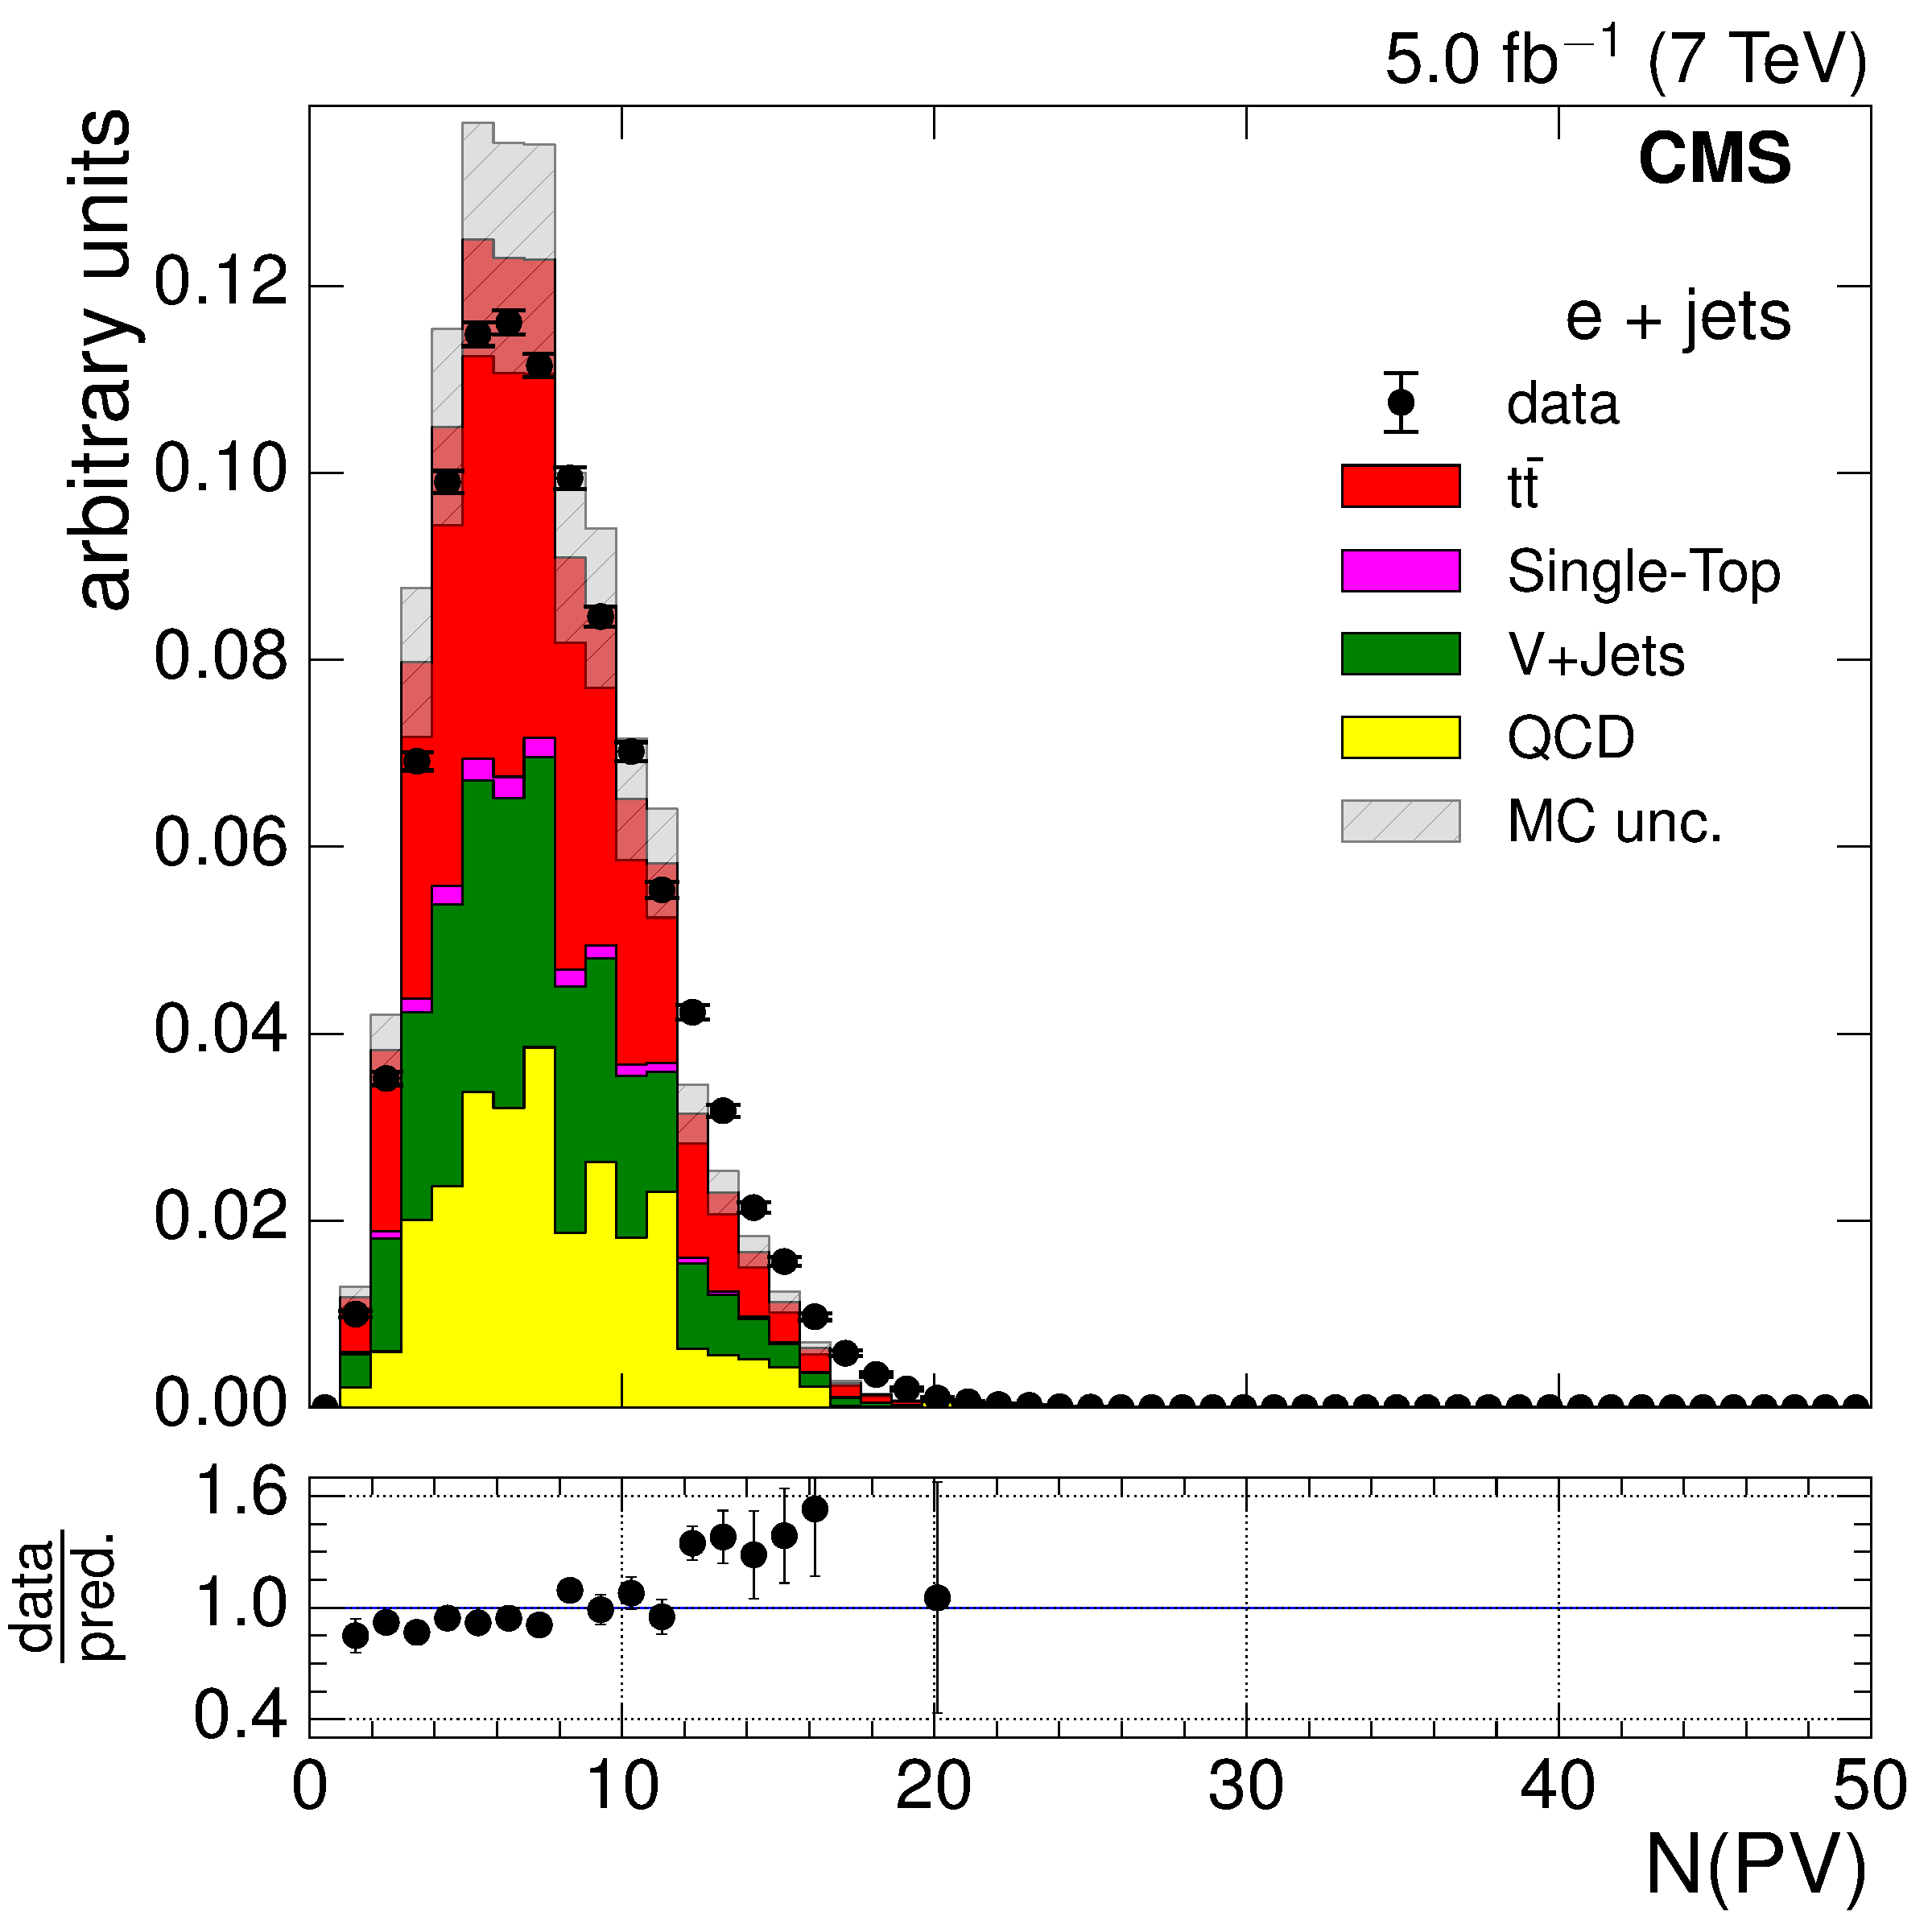
\includegraphics[width=0.48\textwidth]{Chapters/07_08_09_Analysis/Images/control_plots/before_fit/7TeV/EPlusJets_nVertex_with_ratio}\hfill
      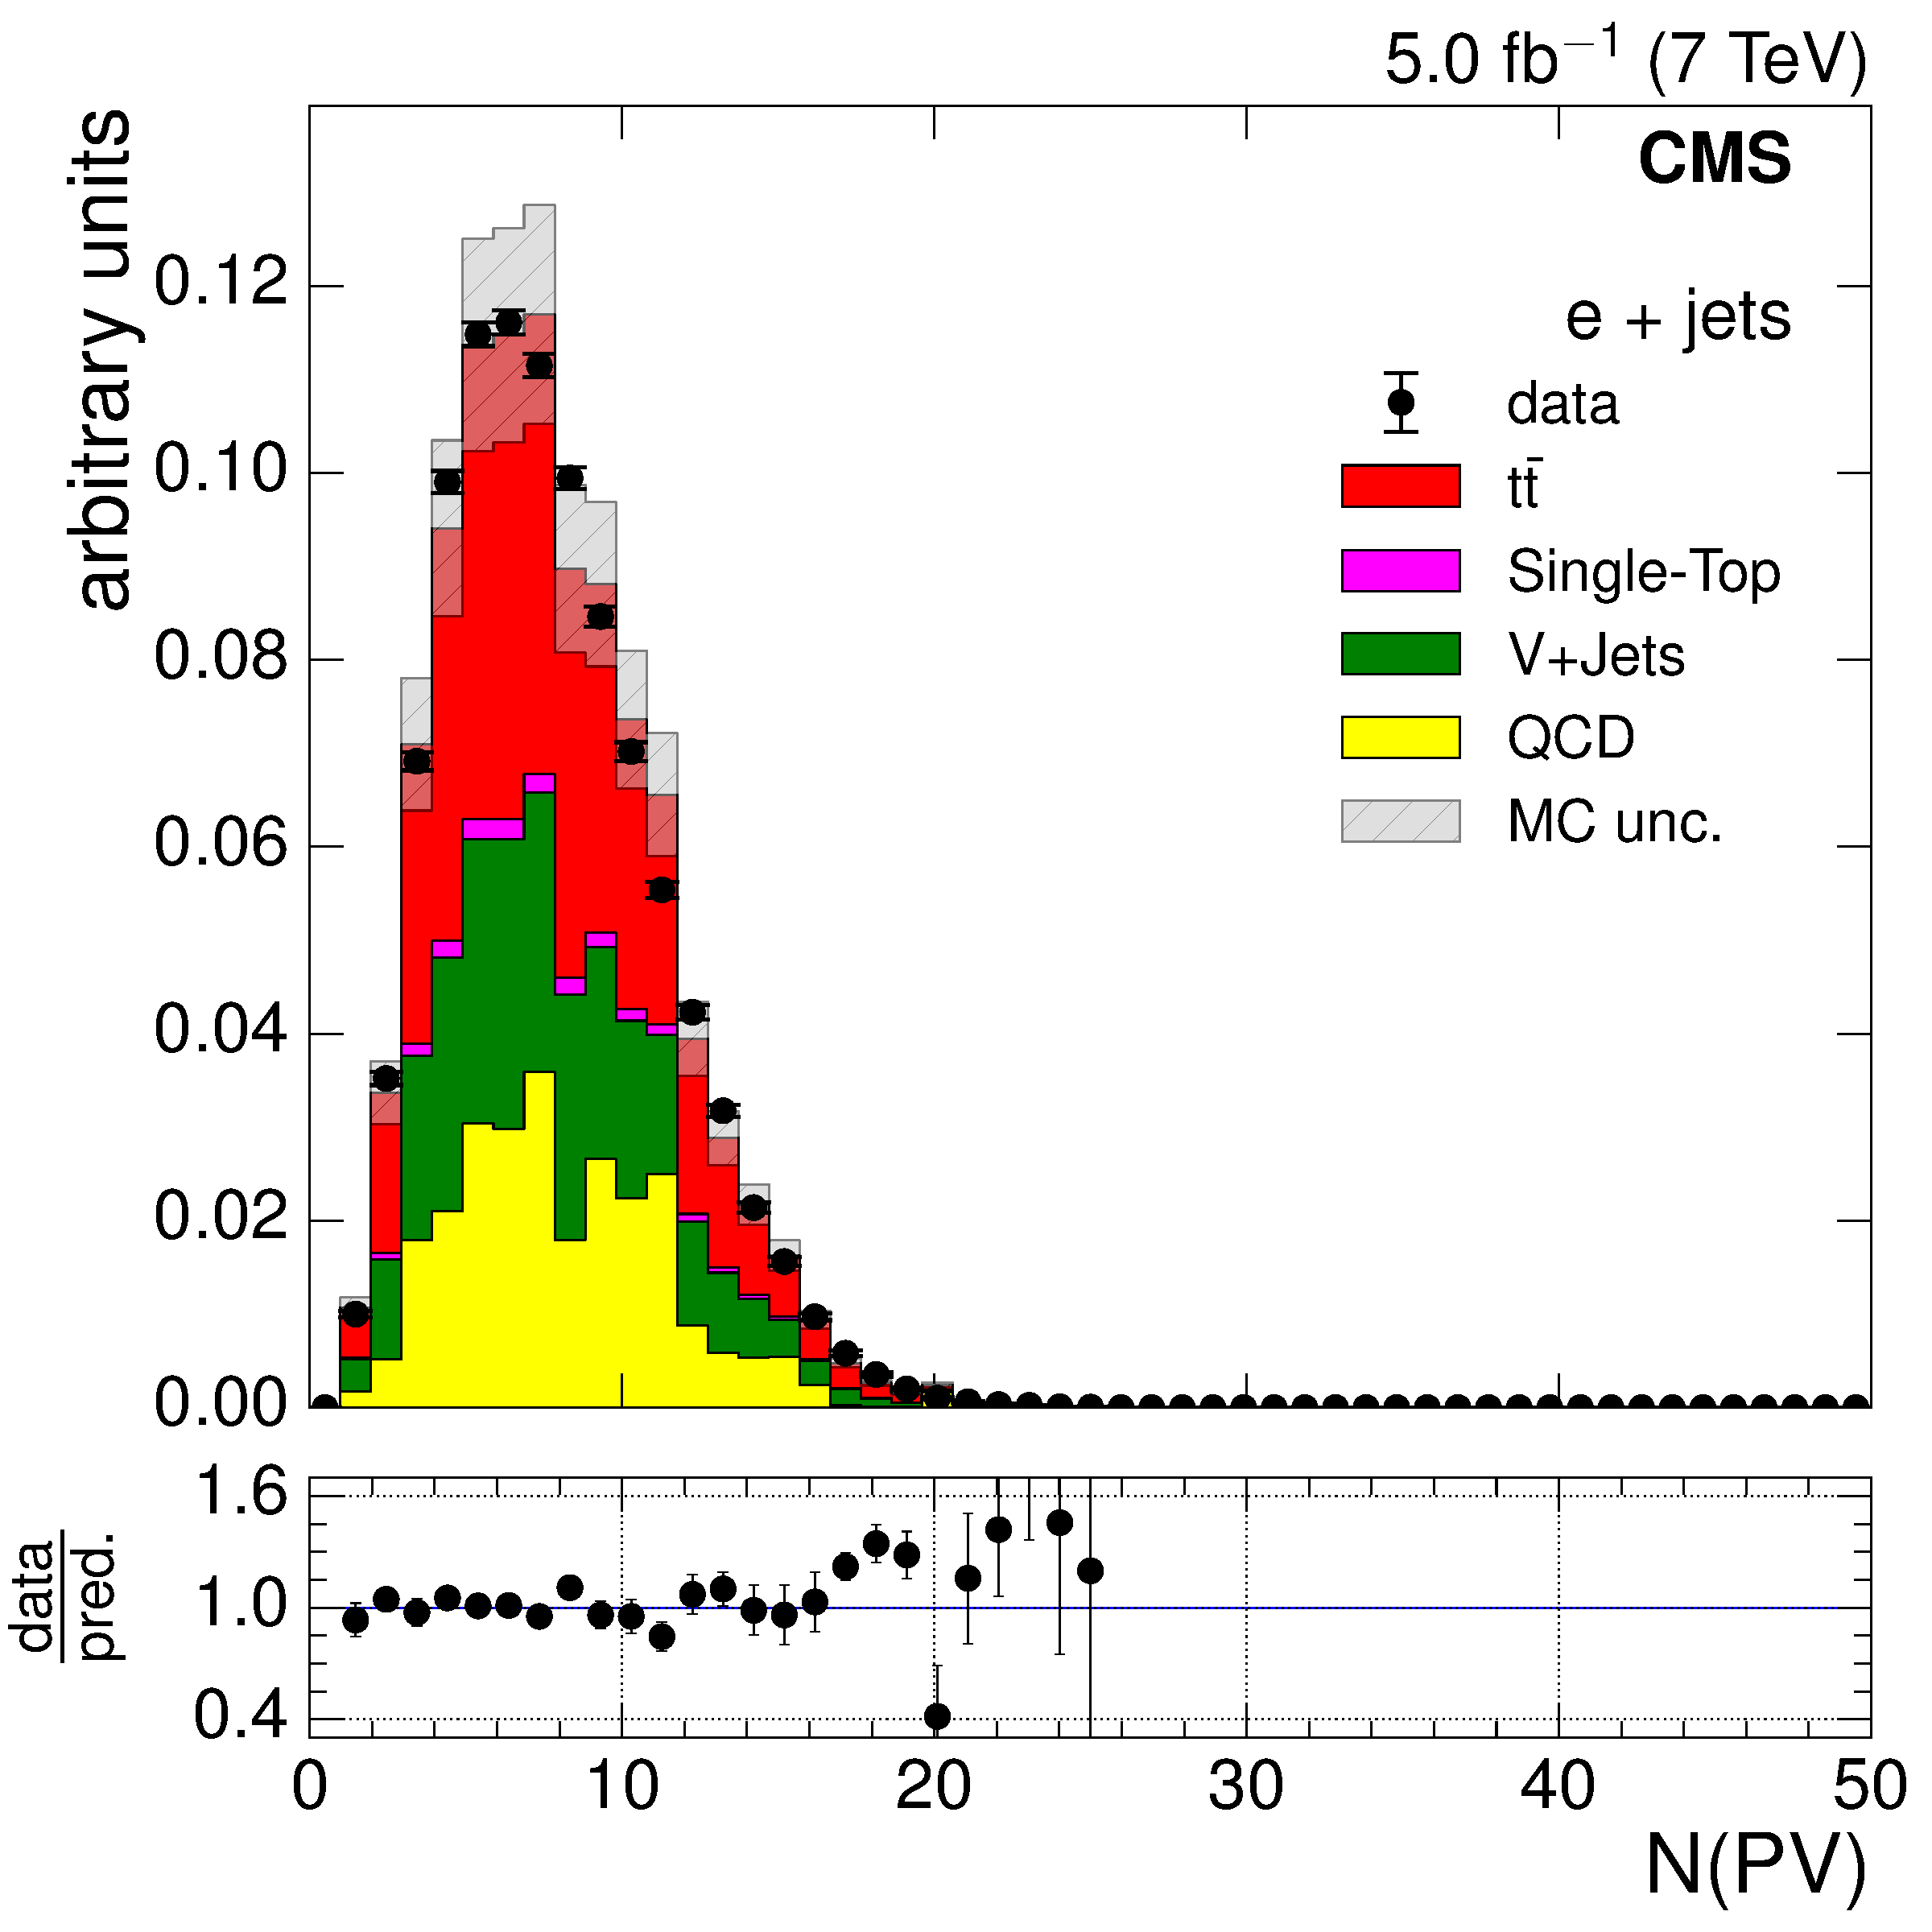
\includegraphics[width=0.48\textwidth]{Chapters/07_08_09_Analysis/Images/control_plots/before_fit/7TeV/EPlusJets_nVertex_reweighted_with_ratio}\\
      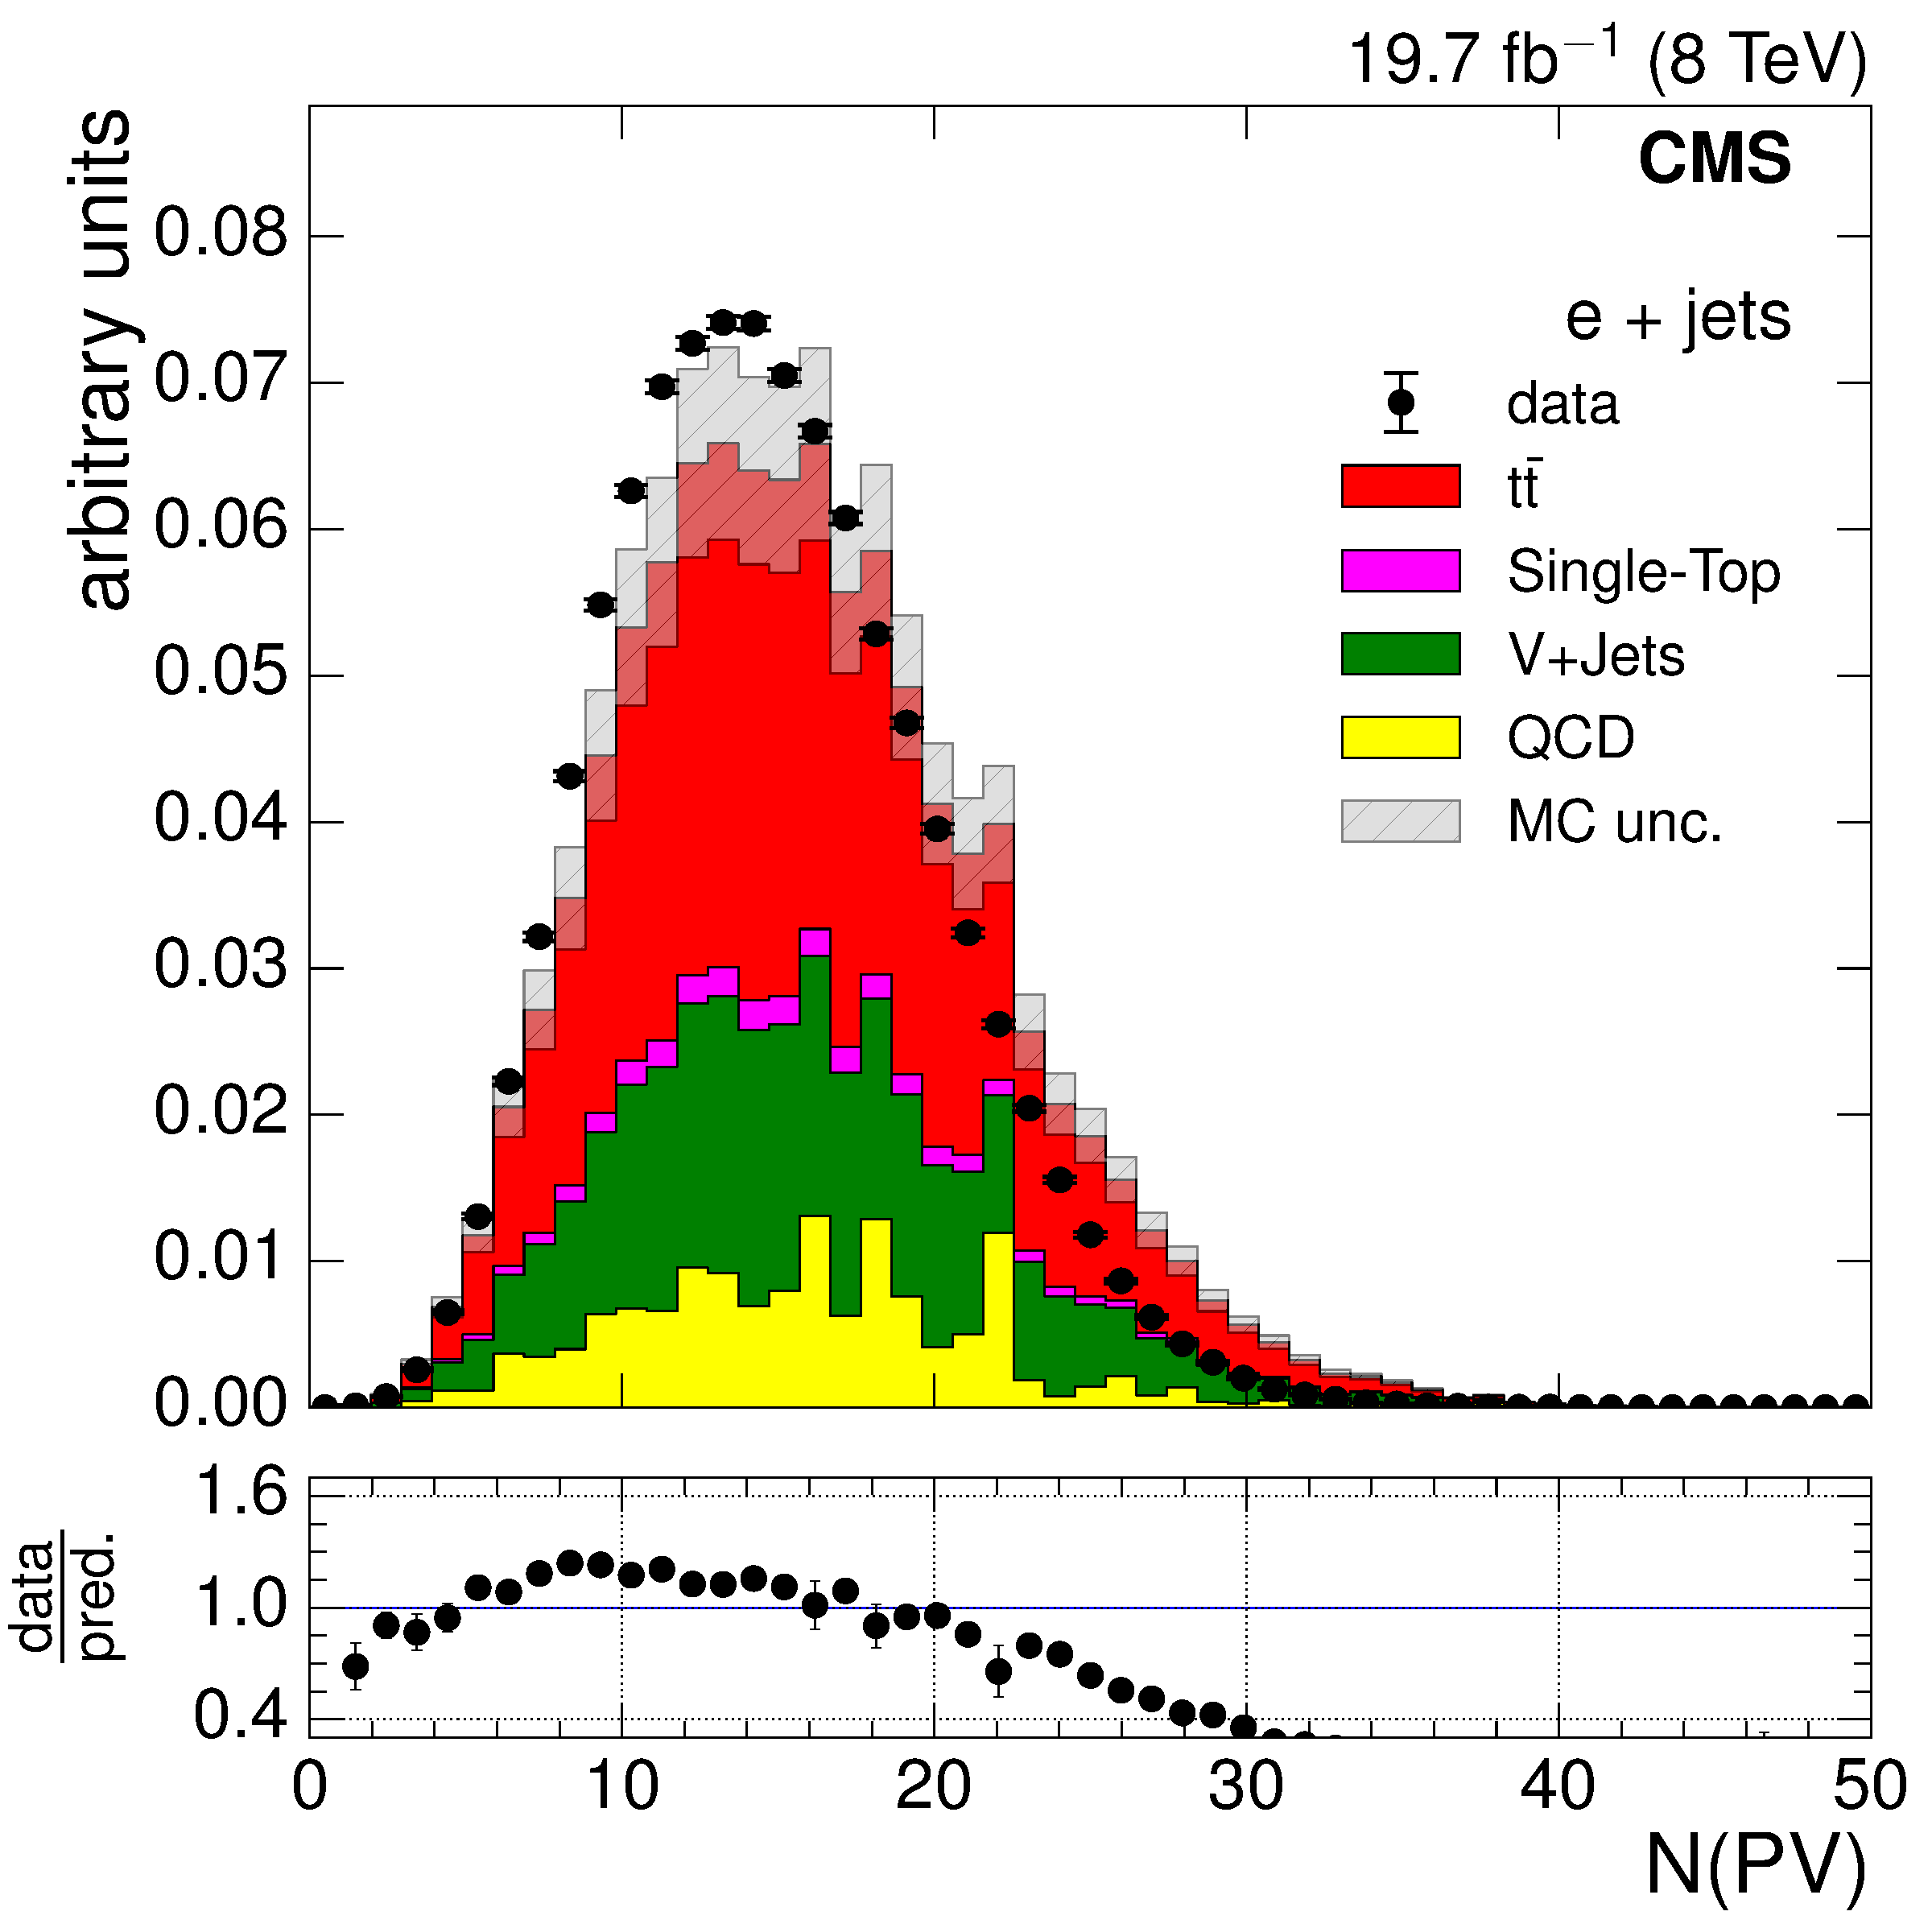
\includegraphics[width=0.48\textwidth]{Chapters/07_08_09_Analysis/Images/control_plots/before_fit/8TeV/EPlusJets_nVertex_with_ratio}\hfill
      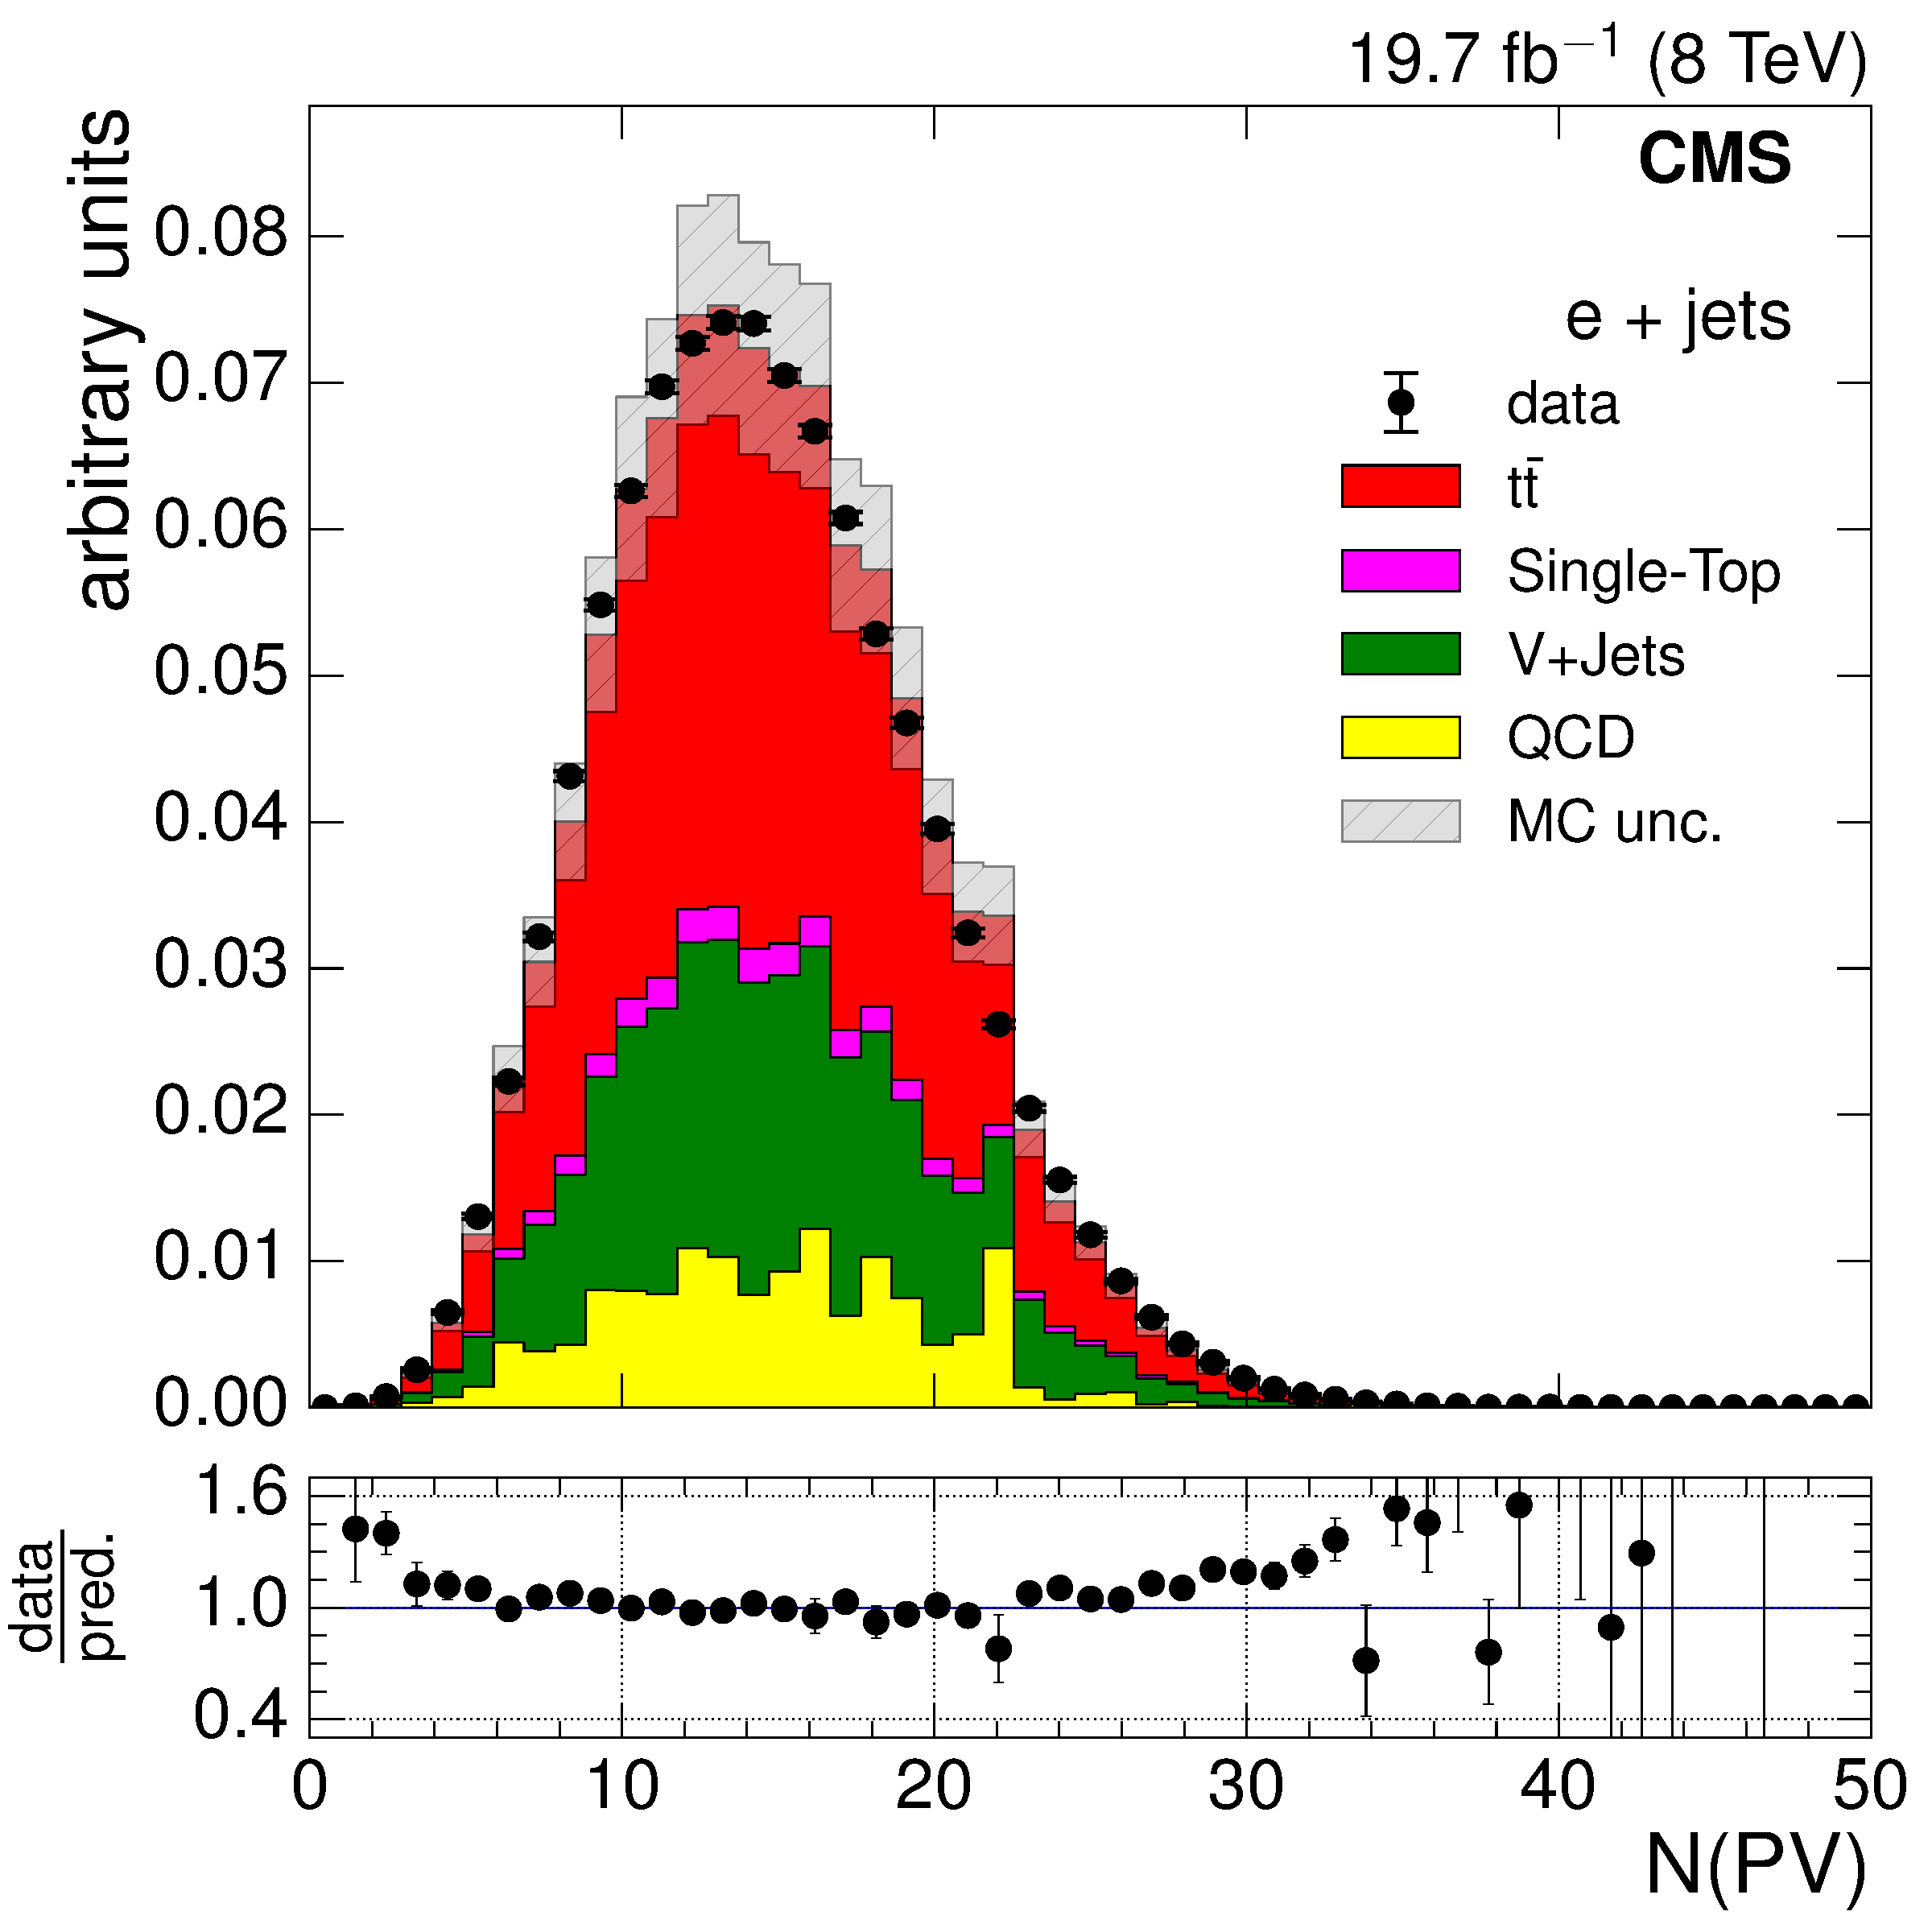
\includegraphics[width=0.48\textwidth]{Chapters/07_08_09_Analysis/Images/control_plots/before_fit/8TeV/EPlusJets_nVertex_reweighted_with_ratio}\\
     \caption[Distributions of the number of reconstructed vertices in an event in the electron+jets channel
     before and after implementing pileup reweighting at $\roots=7\TeV$ and $\roots=8\TeV$.]{Distributions of
     the number of reconstructed vertices in an event in the electron+jets channel before implementing pileup
     reweighting (left) and after implementation (right) at $\roots=7\TeV$ (upper) and $\roots=8\TeV$ (lower).
     Both data and sum of MC simulations are normalised to one.}
     \label{fig:nvertices_before_and_after_pileup_reweighting_electrons}
\end{figure}

\subsection{\btagging}
\label{ss:b_tagging}
The combined secondary vertex \btagging algorithm (CSV) described in
Section~\ref{ss:combined_secondary_vertex} is used in this analysis to identify jets originating from \bquarks
in \ttbar events. The medium working point, CSVM, which corresponds to a cut on the discriminator output by
the algorithm of 0.679, is used in this analysis. This corresponds to a \btagging efficiency of $\approx$70~\%
and a mis-tag efficiency of 1~\% for jets from light quarks ($\cPqu$, $\cPqd$, $\cPqs$) and gluons.
Discrepancies between the \btagging and mis-tagging efficiencies in data and Monte Carlo simulation have been
noted in $\roots=7\TeV$~\cite{Chatrchyan:2012jua} and $\roots=8\TeV$~\cite{CMS-PAS-BTV-13-001}. To account for
these differences, events are reweighted as a function of \pt and $\eta$, based on the recommendation of the
CMS \btagging POG, with the aim of ensuring that the probability of an event passing selection criteria in
simulation matches the probability of an event in data with the same jet(s) passing the same selection. Monte
Carlo simulation events are reweighted by a combination of an efficiency, which accounts for tagging
efficiencies of \bjets, \cjets and light jets in simulation, and a scale factor, which takes into account the
difference in the aforementioned efficiencies in simulation and data. The result of this reweighting in the
electron+jets channel is shown in Figure~\ref{fig:nbjets_before_and_after_btag_scale_factors_electrons}, and
in the muon+jets channel in Figure~\ref{fig:nbjets_before_and_after_btag_scale_factors_muons} in
Appendix~\ref{as:data_monte_carlo_corrections}. The \btagging efficiency uncertainty is evaluated by varying
the scale factors by $\pm1\sigma$.

\begin{figure}[hbtp]
    \centering
      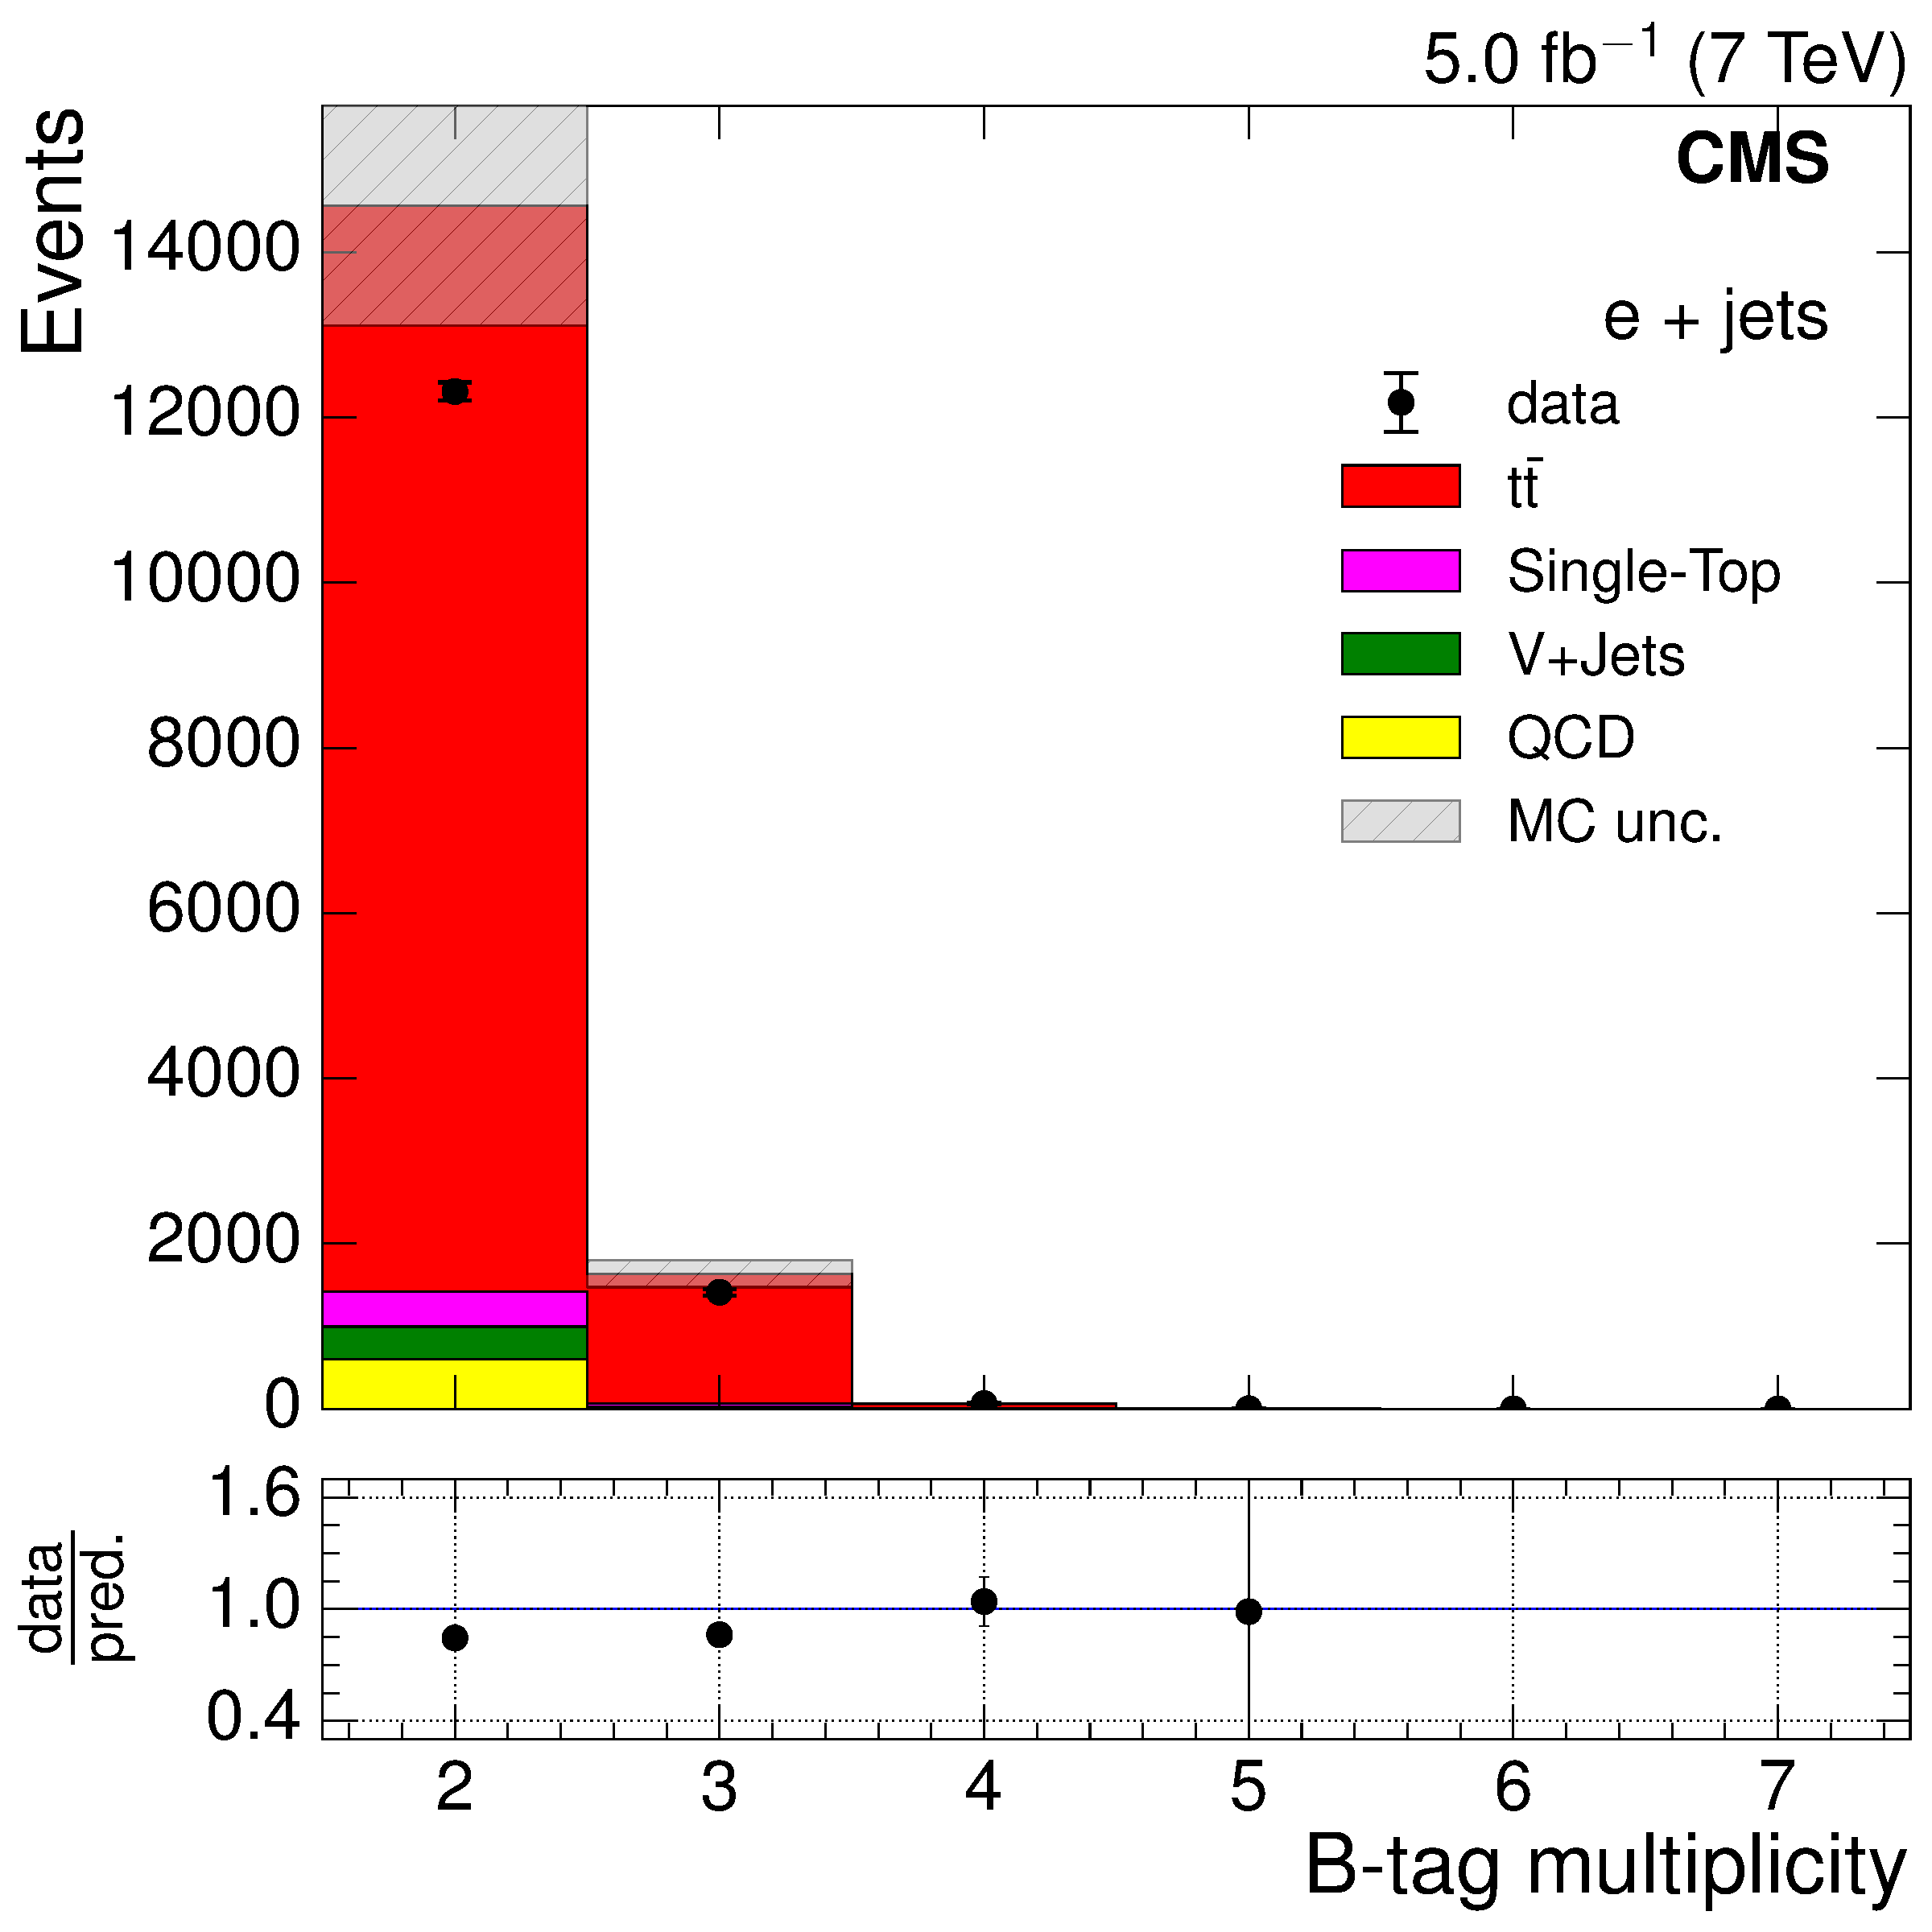
\includegraphics[width=0.48\textwidth]{Chapters/07_08_09_Analysis/Images/control_plots/before_fit/7TeV/EPlusJets_N_BJets_with_ratio}\hfill
      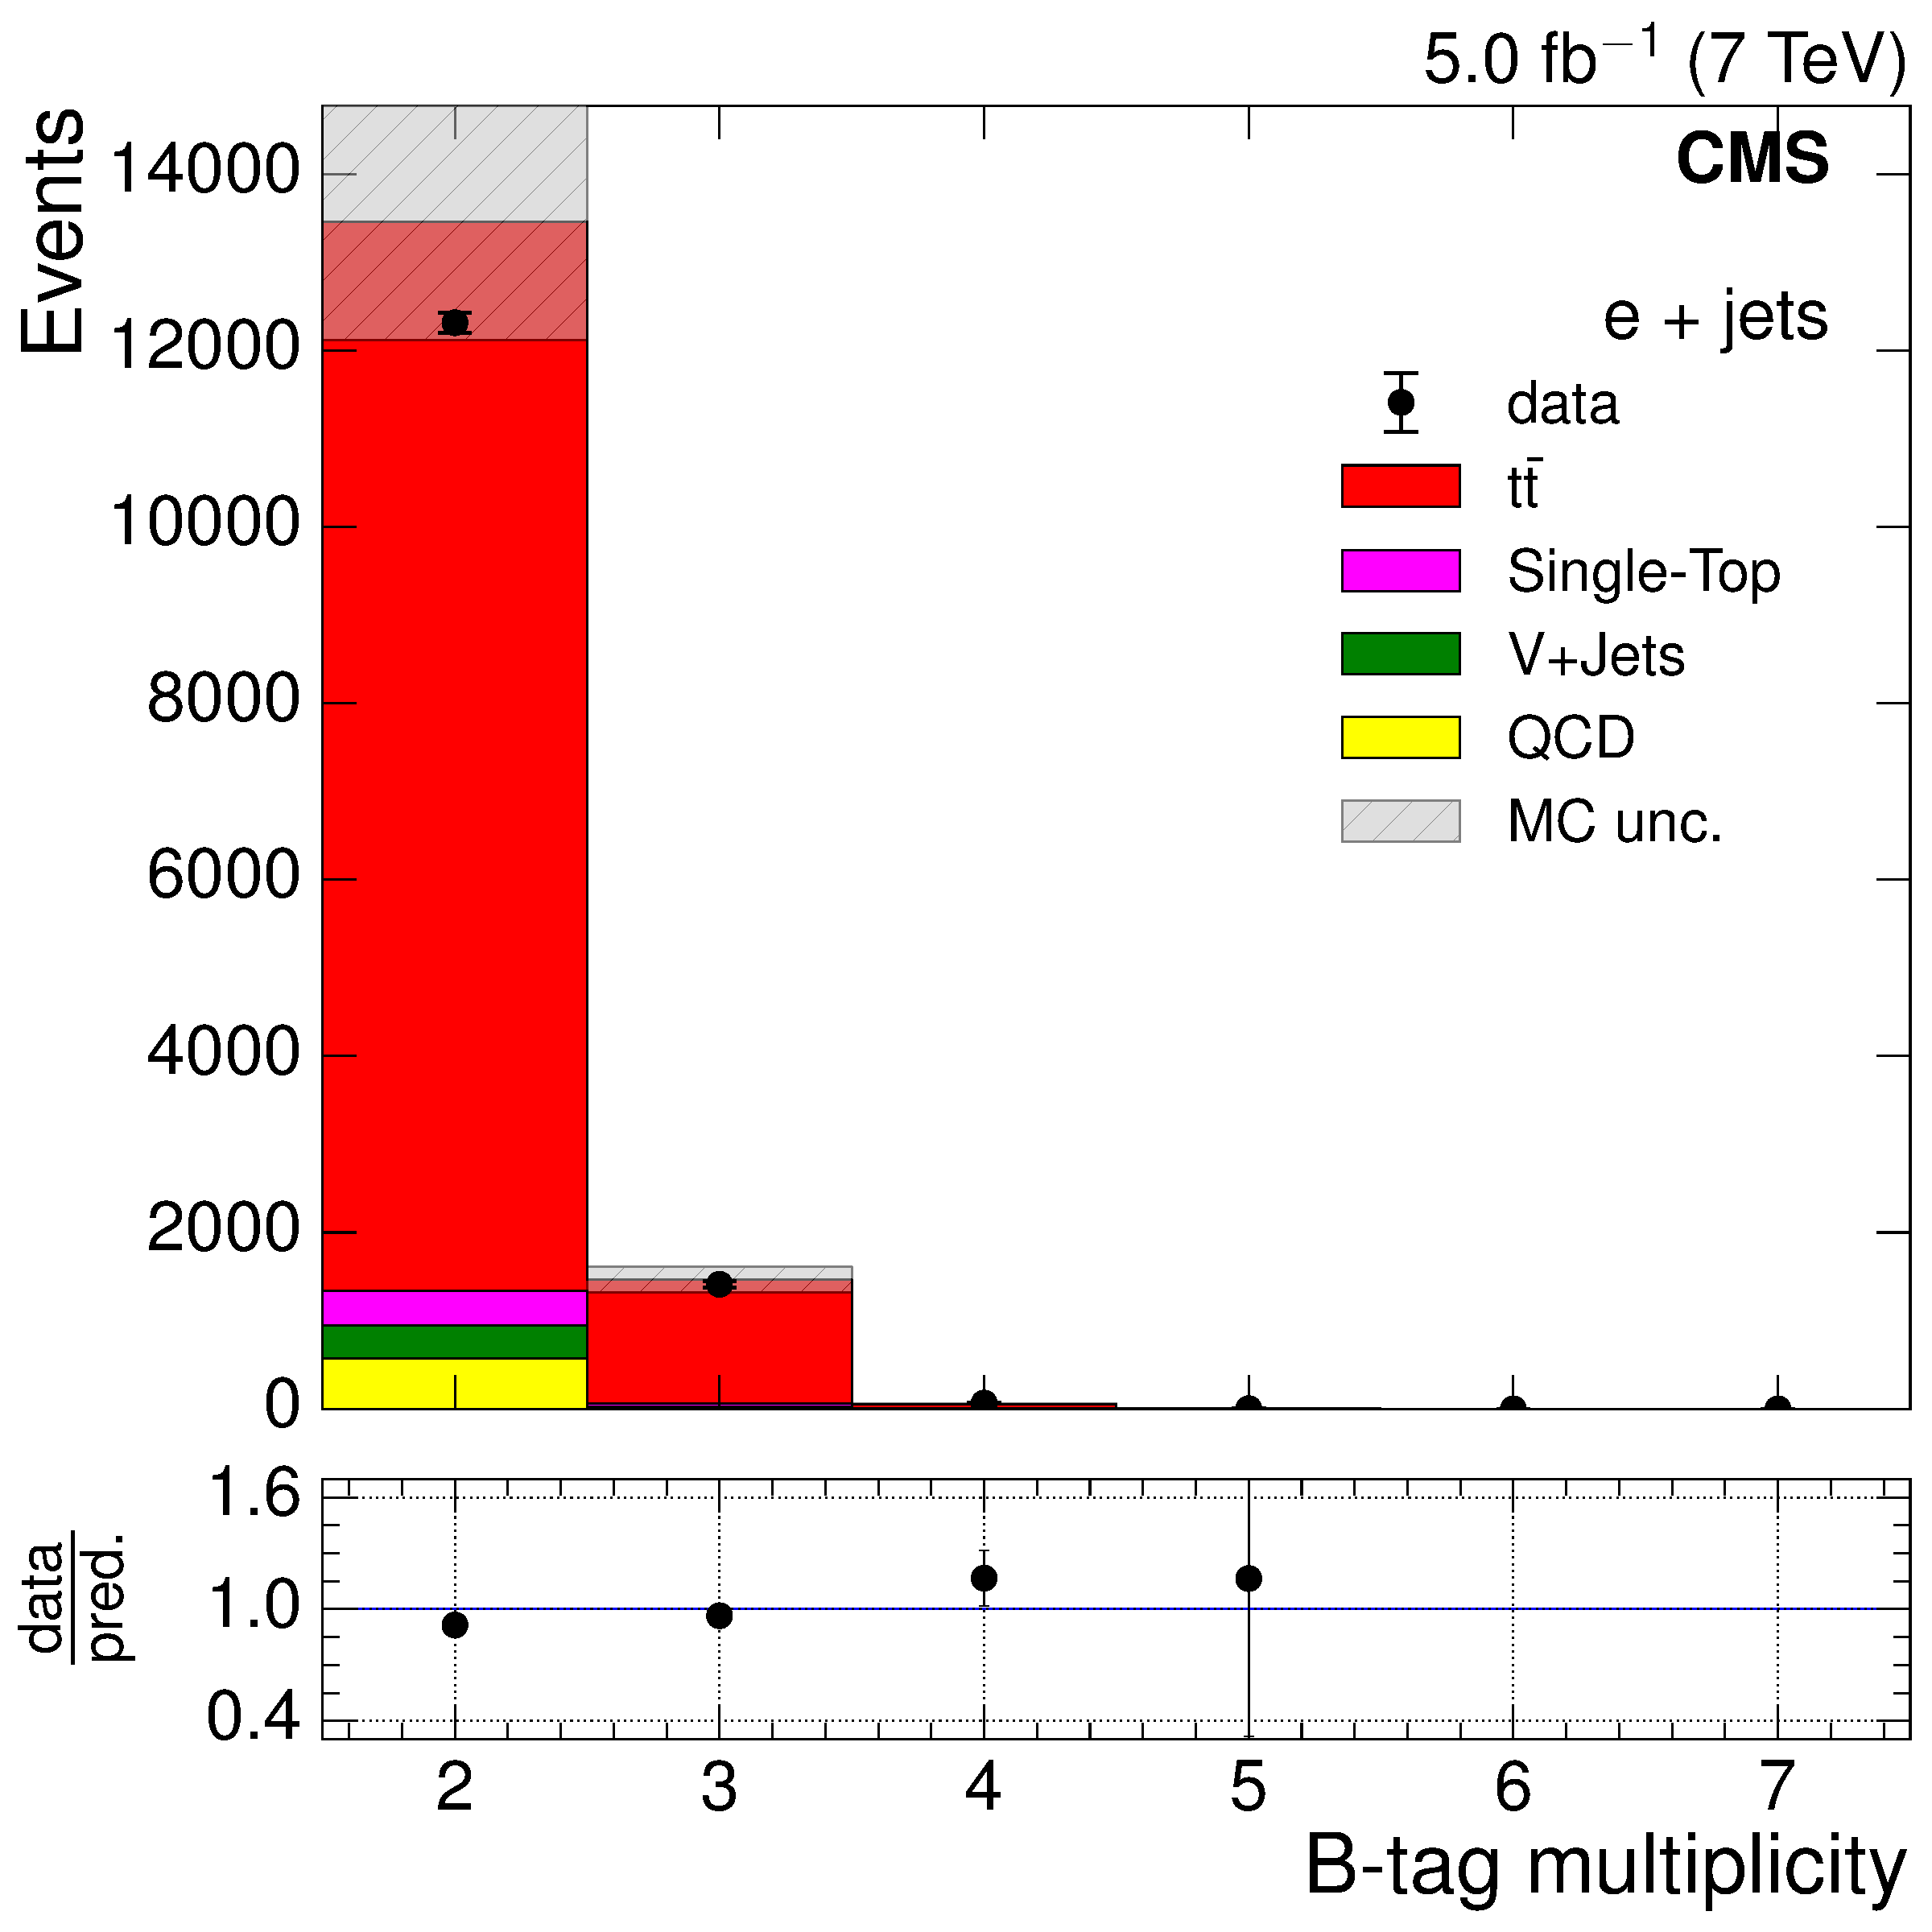
\includegraphics[width=0.48\textwidth]{Chapters/07_08_09_Analysis/Images/control_plots/before_fit/7TeV/EPlusJets_N_BJets_reweighted_with_ratio}\\
      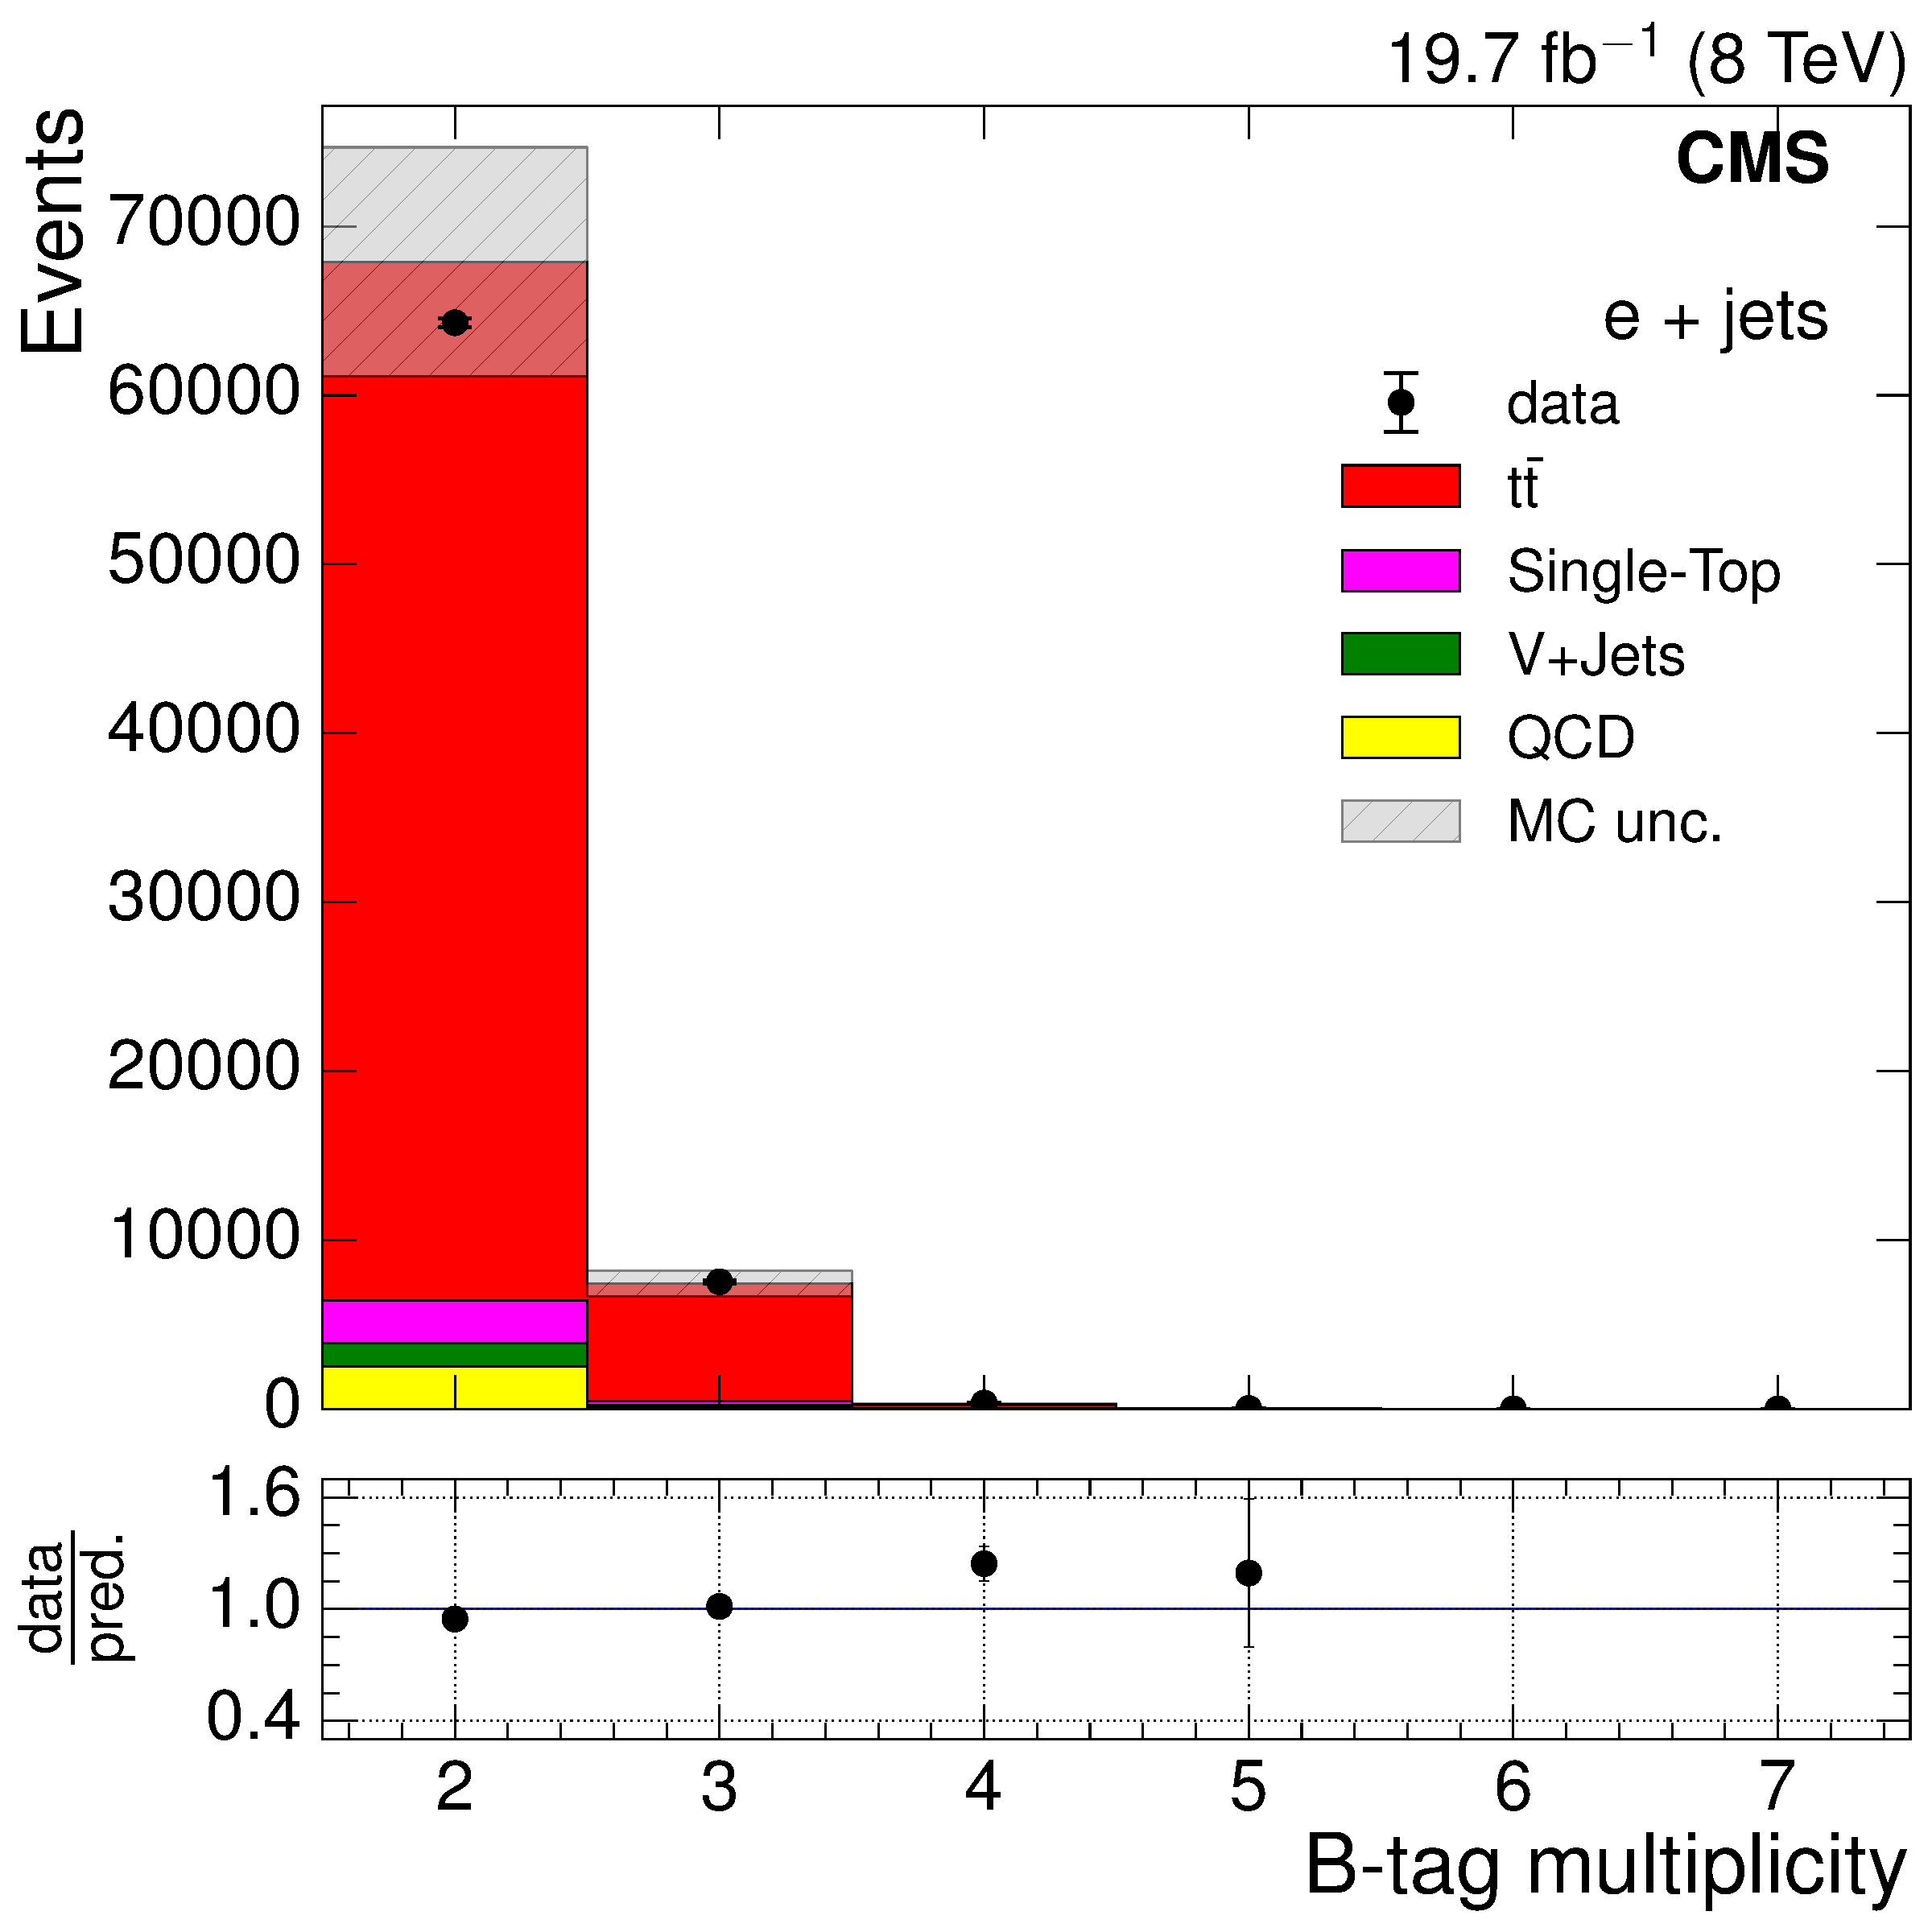
\includegraphics[width=0.48\textwidth]{Chapters/07_08_09_Analysis/Images/control_plots/before_fit/8TeV/EPlusJets_N_BJets_with_ratio}\hfill
      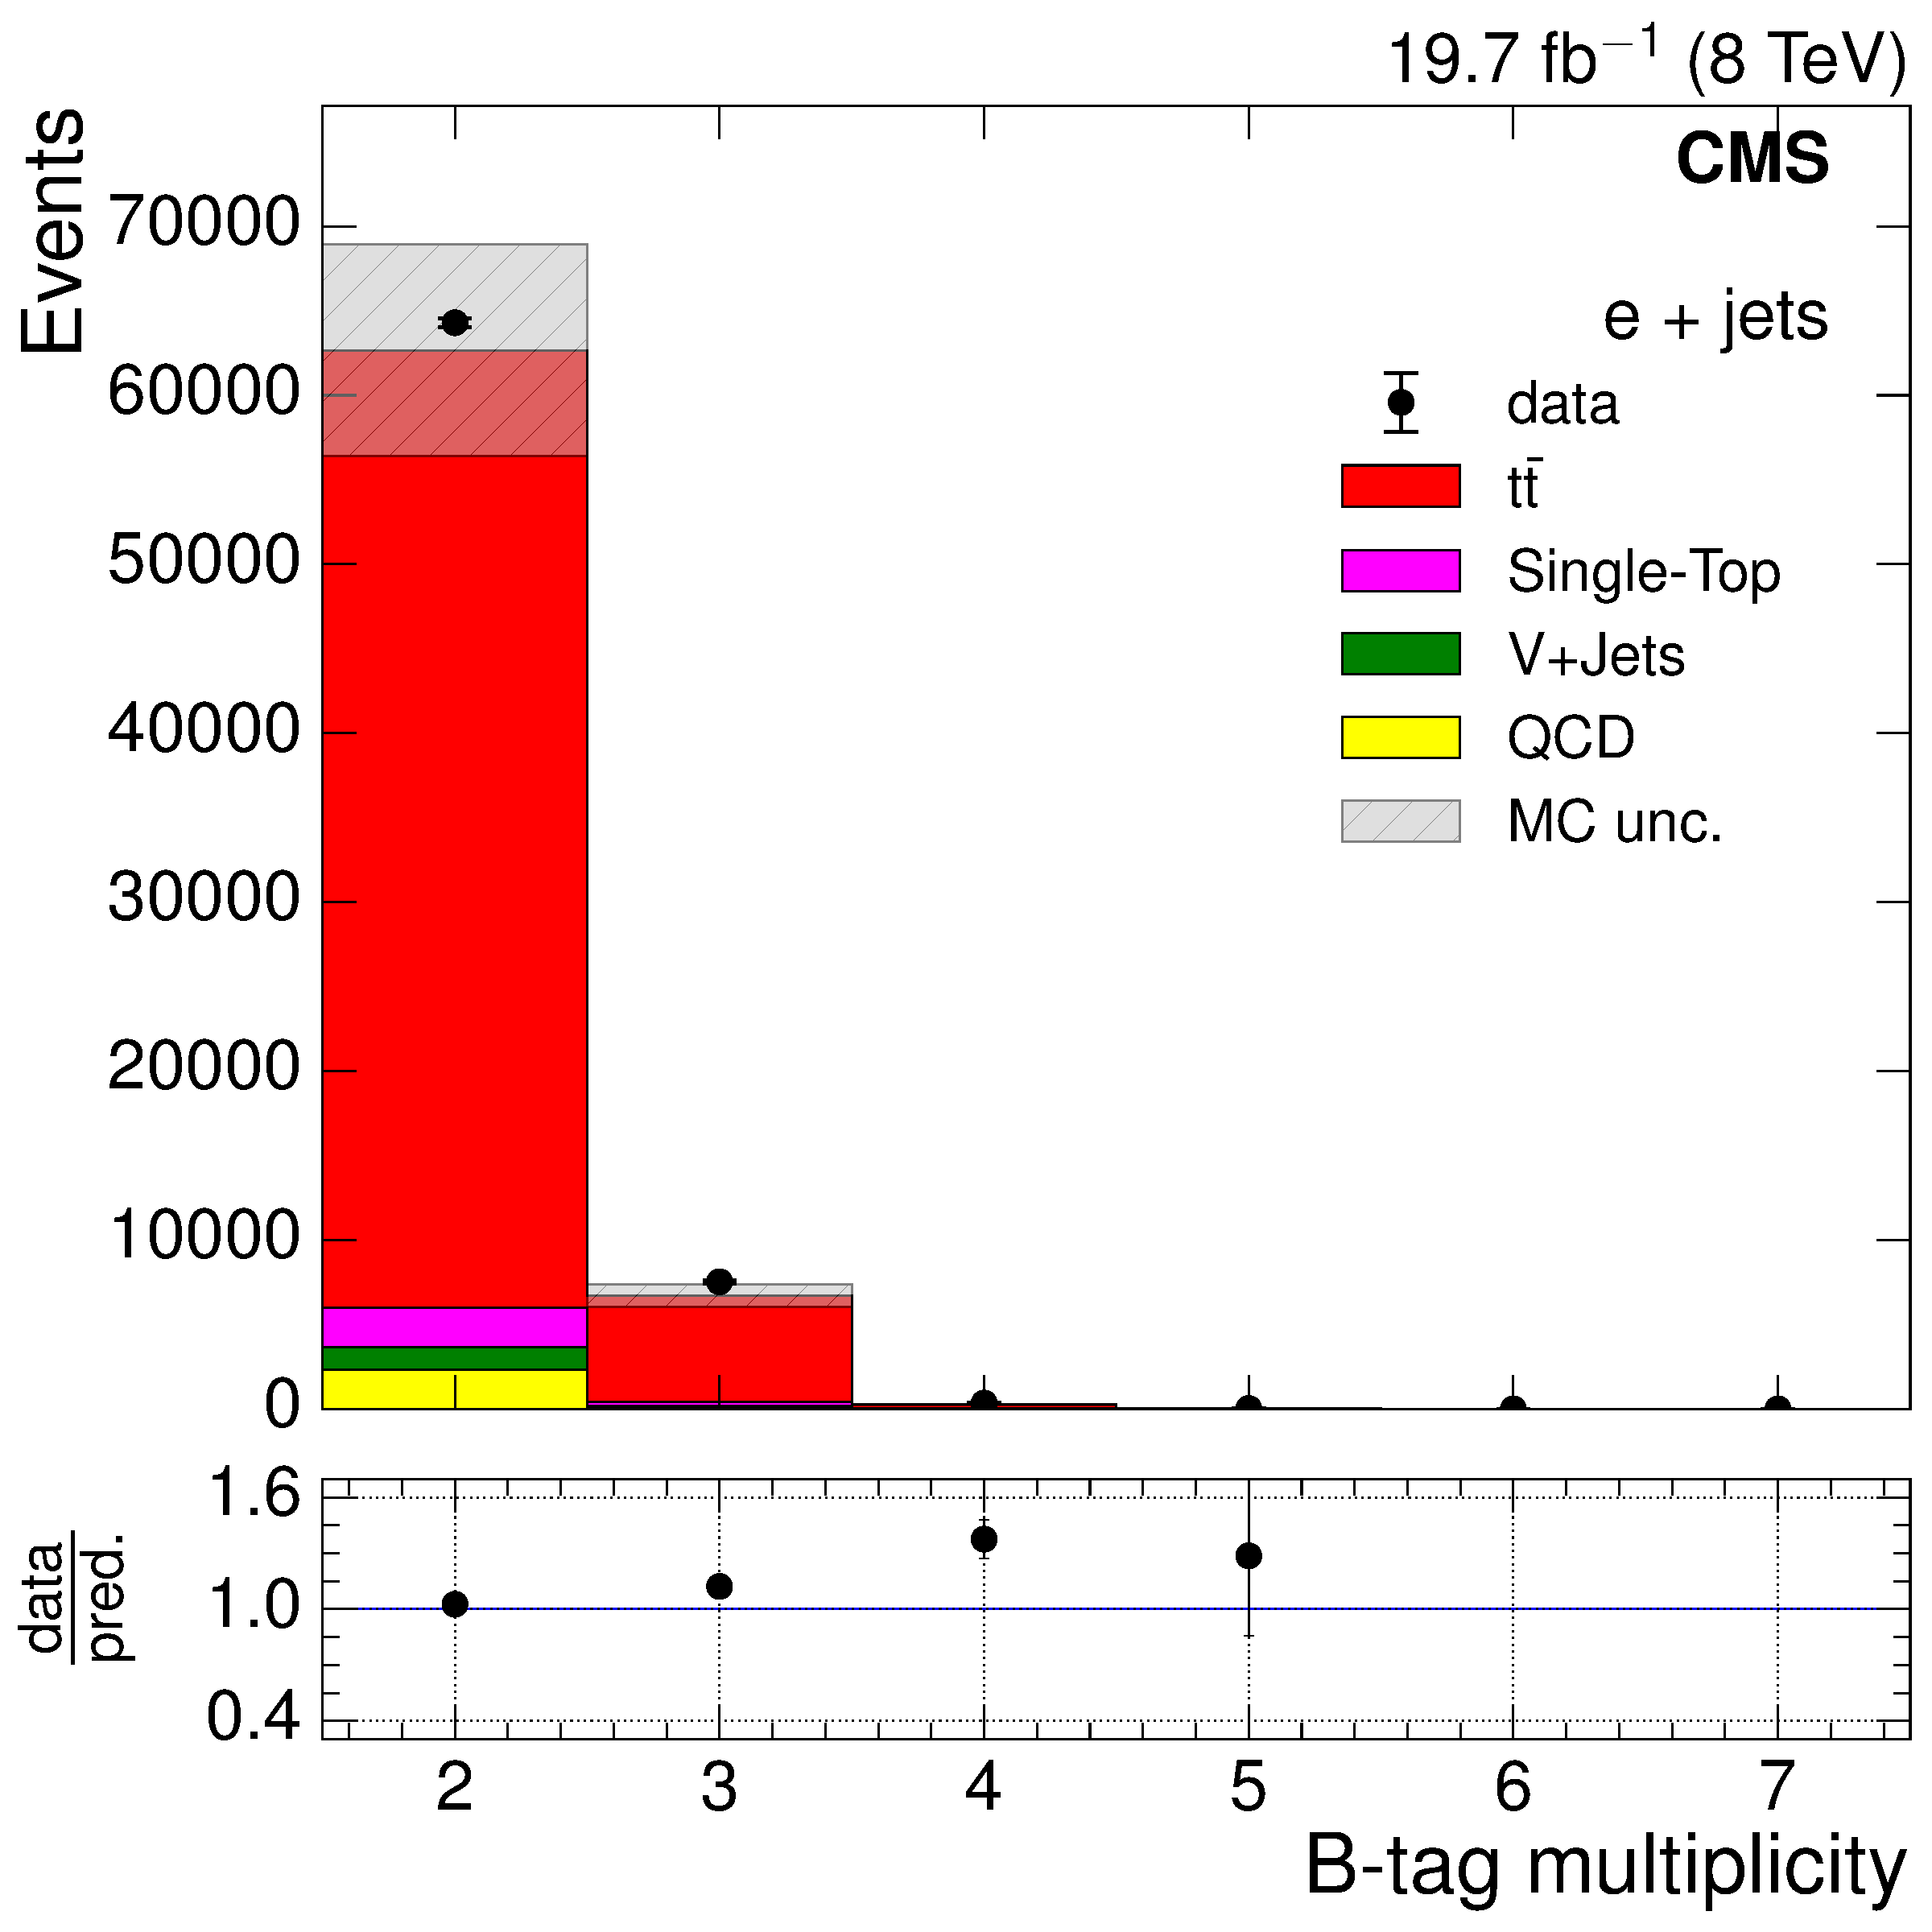
\includegraphics[width=0.48\textwidth]{Chapters/07_08_09_Analysis/Images/control_plots/before_fit/8TeV/EPlusJets_N_BJets_reweighted_with_ratio}\\
     \caption[Distributions of the number of \btags in an event in the electron+jets channel before
     and after applying \btag scale factors at $\roots=7\TeV$ and $\roots=8\TeV$.]{Distributions of
     the number of \btags in an event in the electron+jets channel before applying \btag scale factors (left)
     and after application (right) at $\roots=7\TeV$ (upper) and $\roots=8\TeV$ (lower).}
     \label{fig:nbjets_before_and_after_btag_scale_factors_electrons}
\end{figure}

%TODO: mention also not important because of fitting?

\subsection{Jet Energy Scale}
\label{sss:jet_energy_scale}
Jet energies are corrected to take into account energy coming from other sources. Level 1 (L1 Pileup)
corrections remove energy that comes from pileup collisions, Level 2 (L2 Relative) corrections remove the
dependence of jet response on $\eta$, and Level 3 (L3 Absolute) corrections correct for the jet response
dependence on \pt~\cite{Chatrchyan:2011ds}. These corrections are applied to both data and Monte Carlo
simulation events. An additional residual correction (L2L3Residual) is applied to data only for fine tuning of
the agreement between data and simulation.

Furthermore, jet energy resolution corrections are applied to simulation (known as jet smearing) to account
for the fact that jet energy resolution has been measured to be worse in data than in simulation. These PF jet
corrections are provided by the CMS JETMET Physics Object Group using 0.8\fbinv of dijet data at
$\roots=7\TeV$~\cite{Chatrchyan:2011ds} and 19.7\fbinv of dijet data at $\roots=8\TeV$~\cite{jet_res_2012}.

\subsection{Missing Transverse Energy Corrections}
\label{ss:met_corrections}

No selection criteria is placed on missing transverse energy in an event, but corrections are applied to \met
as follows. selection The adjustments to the jet energies as a result of the corrections mentioned in
Section~\ref{sss:jet_energy_scale} in turn affect the distributions of \met in the event.
Corrections known as Type-I \met corrections are applied to propagate these changes to the \met distributions
in the case of jets $\geq10\GeV$. In addition, Type-0 corrections are applied to account for pileup
interactions in the event by carrying out charged hadron subtraction (the removal of charged hadrons coming
pileup vertices). Finally, a known issue causing a roughly sinusoidal modulation of the \met distribution with
respect to $\phi$ in both simulation and data, is mitigated by applying \met $\phi$ corrections. This
correction ensures the \met distribution is independent of $\phi$, due to the rotational symmetry of
collisions around the beam axis.
 
\subsection{Trigger, Lepton ID and Isolation Efficiencies and Corrections}
\label{ss:trigger_ID_isolation_corrections}
Corrections are also required for the trigger, identification and isolation efficiencies for muons and
electrons. In the muon+jets channel, the corrections were provided by the CMS muon POG for $\roots=8\TeV$
%TODO:FINDREF (ONLY A TWIKI, WOULD THIS BE OK?)
and $\roots=7\TeV$~\cite{CMS-PAS-SMP-13-013}.

For the electron+jets channel, the corrections were provided by the CMS EGamma Physics Object Group for
$\roots=8\TeV$, %TODO:FINDREF (ONLY A TWIKI, WOULD THIS BE OK?)
however the corrections for the $\roots=7\TeV$ data were not provided and so were derived independently in
this analysis using the same tag and probe methods as used by the EGamma POG.

The 7\TeV triggers used (ElectronHad) in this analysis were not present in the 7\TeV simulation,
and so the trigger efficiency was calculated with respect to the full selection. This efficiency was then
implemented in the Monte Carlo simulation, thereby imitating the trigger. It should be noted that it is
assumed that the electron and hadron legs of the trigger are not correlated, since electrons are cleaned from
the jet collection at HLT level.

A tag and probe method~\cite{CMS:2011aa} was used to derive identification, isolation scale factors and
electron trigger efficiencies. The full reference selection was first applied with the exception of trigger,
\btagging and electron veto requirements, while in addition, a second loose electron was required. A \Z mass
constraint was placed on the two electrons in the event by requiring them to have an invariant mass of between
60\GeV and 120\GeV, thus ensuring that the pair of electrons originated from a \Z boson decay. The tight
(`tag') electron requirements were \pt$>30\GeV$, $\abseta<0.8$, relative isolation <0.1, MVA
identification$>0.9$, $d_{xy}<0.02\cm$ and reconstructed at HLT level. The loose (`probe') electron
requirements were $\pt>30\GeV$, $\abseta<2.5$ and $d_{xy}<2\cm$.

Fits were then performed, firstly of the invariant mass of all pairs of tag and probe electrons, and secondly
after applying the identification and isolation criteria to the probe electrons, to the invariant mass
distribution of pairs of tag and probe electrons in which the probe electron passed the identification and
isolation criteria. The fit was implemented in both Monte Carlo simulation and in data, and a Breit-Wigner
distribution convoluted with a Crystal Ball function is used to model the invariant mass of the tag and probe
electrons, with a falling exponential used to model the background distribution. The Breit-Wigner distribution
takes a form similar to that of a Gaussian distribution, with flatter tails~\cite{PhysRev.49.519}. The Crystal
Ball function is also based on a Gaussian distribution, but with a power-law tail to the lower end
~\cite{Oreglia,Gaiser,Skwarnicki}. Both of these functions are commonly used to model the mass peaks of
resonances. The result of this fitting procedure in data can be seen in
Figure~\ref{fig:electron_id_iso_efficiency_invariant_Z_mass_fits_data}.

\begin{figure}[hbtp]
    \centering
      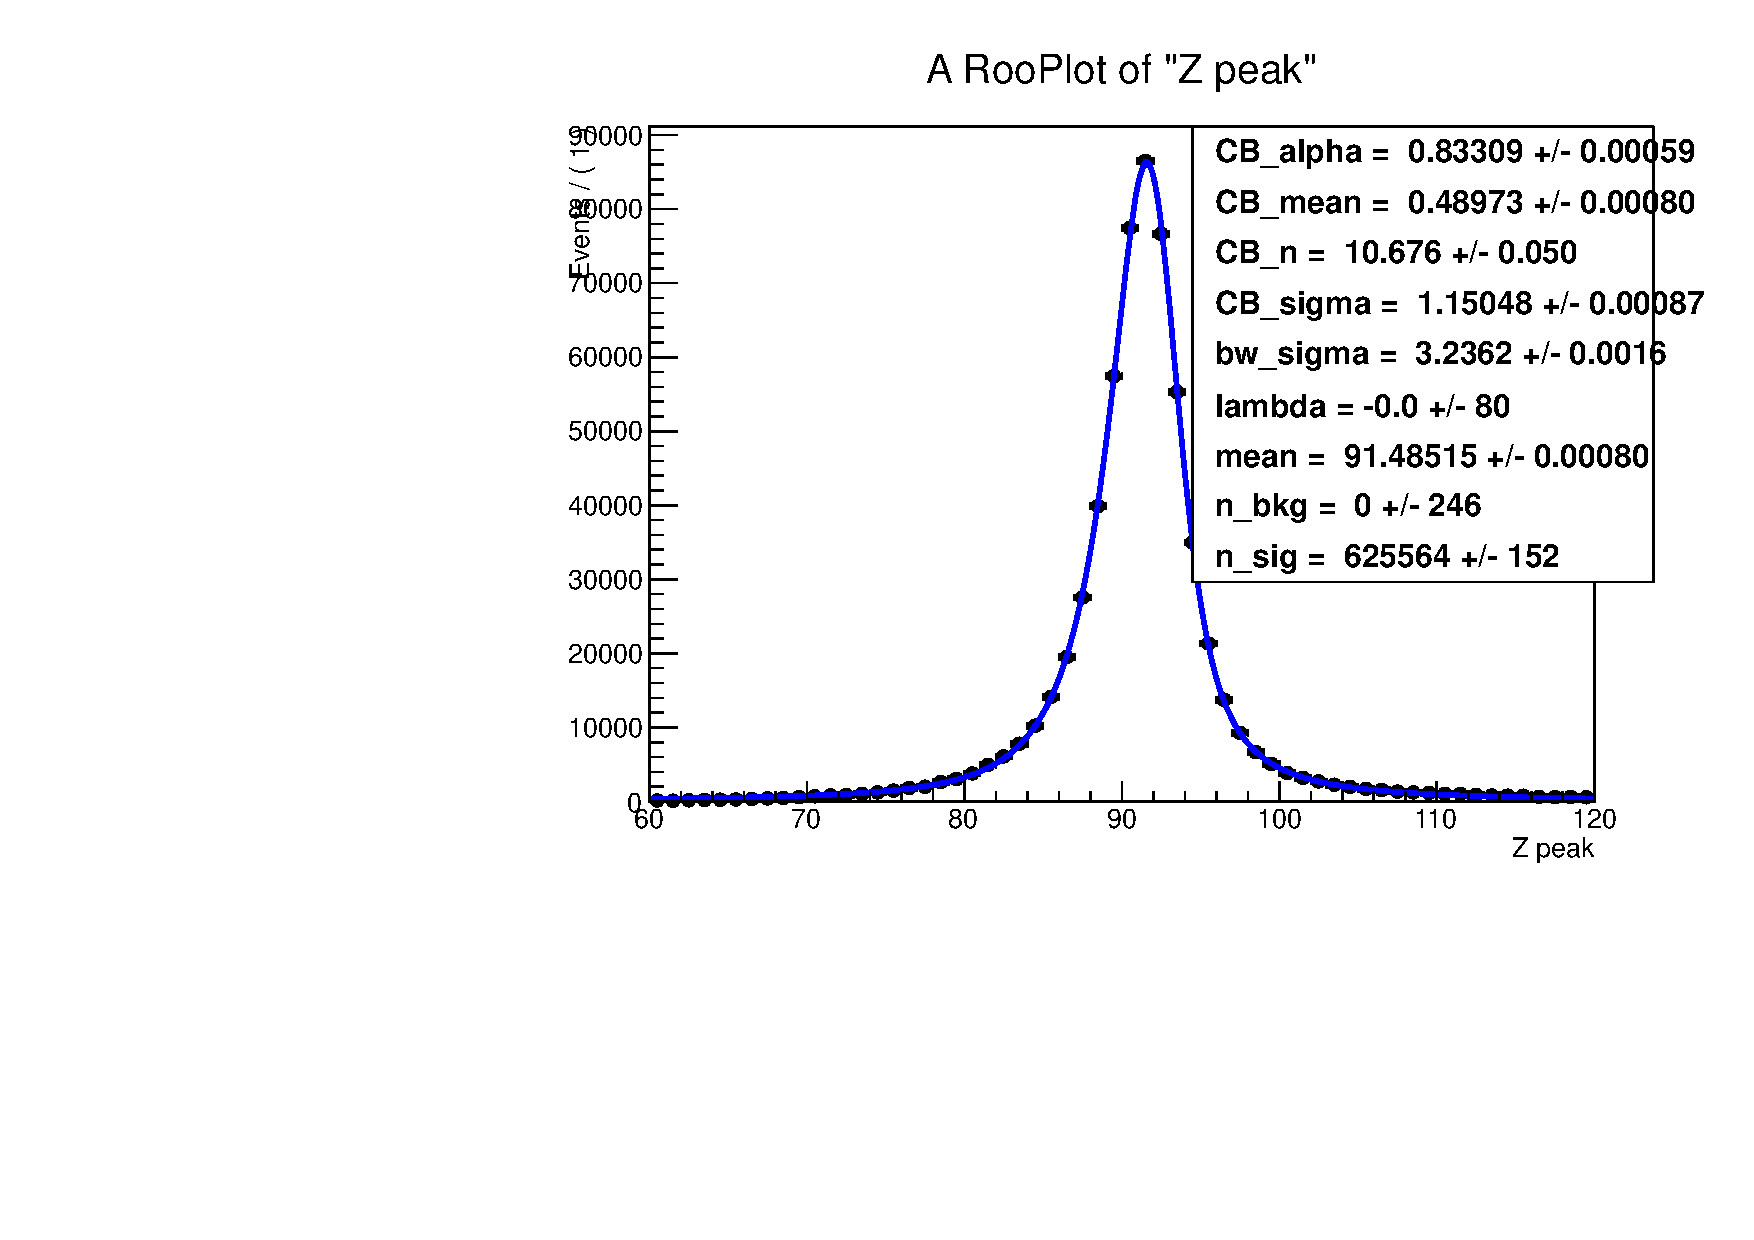
\includegraphics[width=0.48\textwidth]{Chapters/07_08_09_Analysis/Images/lepton_scale_factors/CBConvolution/electron/data/id_iso/tagProbe_total_Z_peak}\hfill
      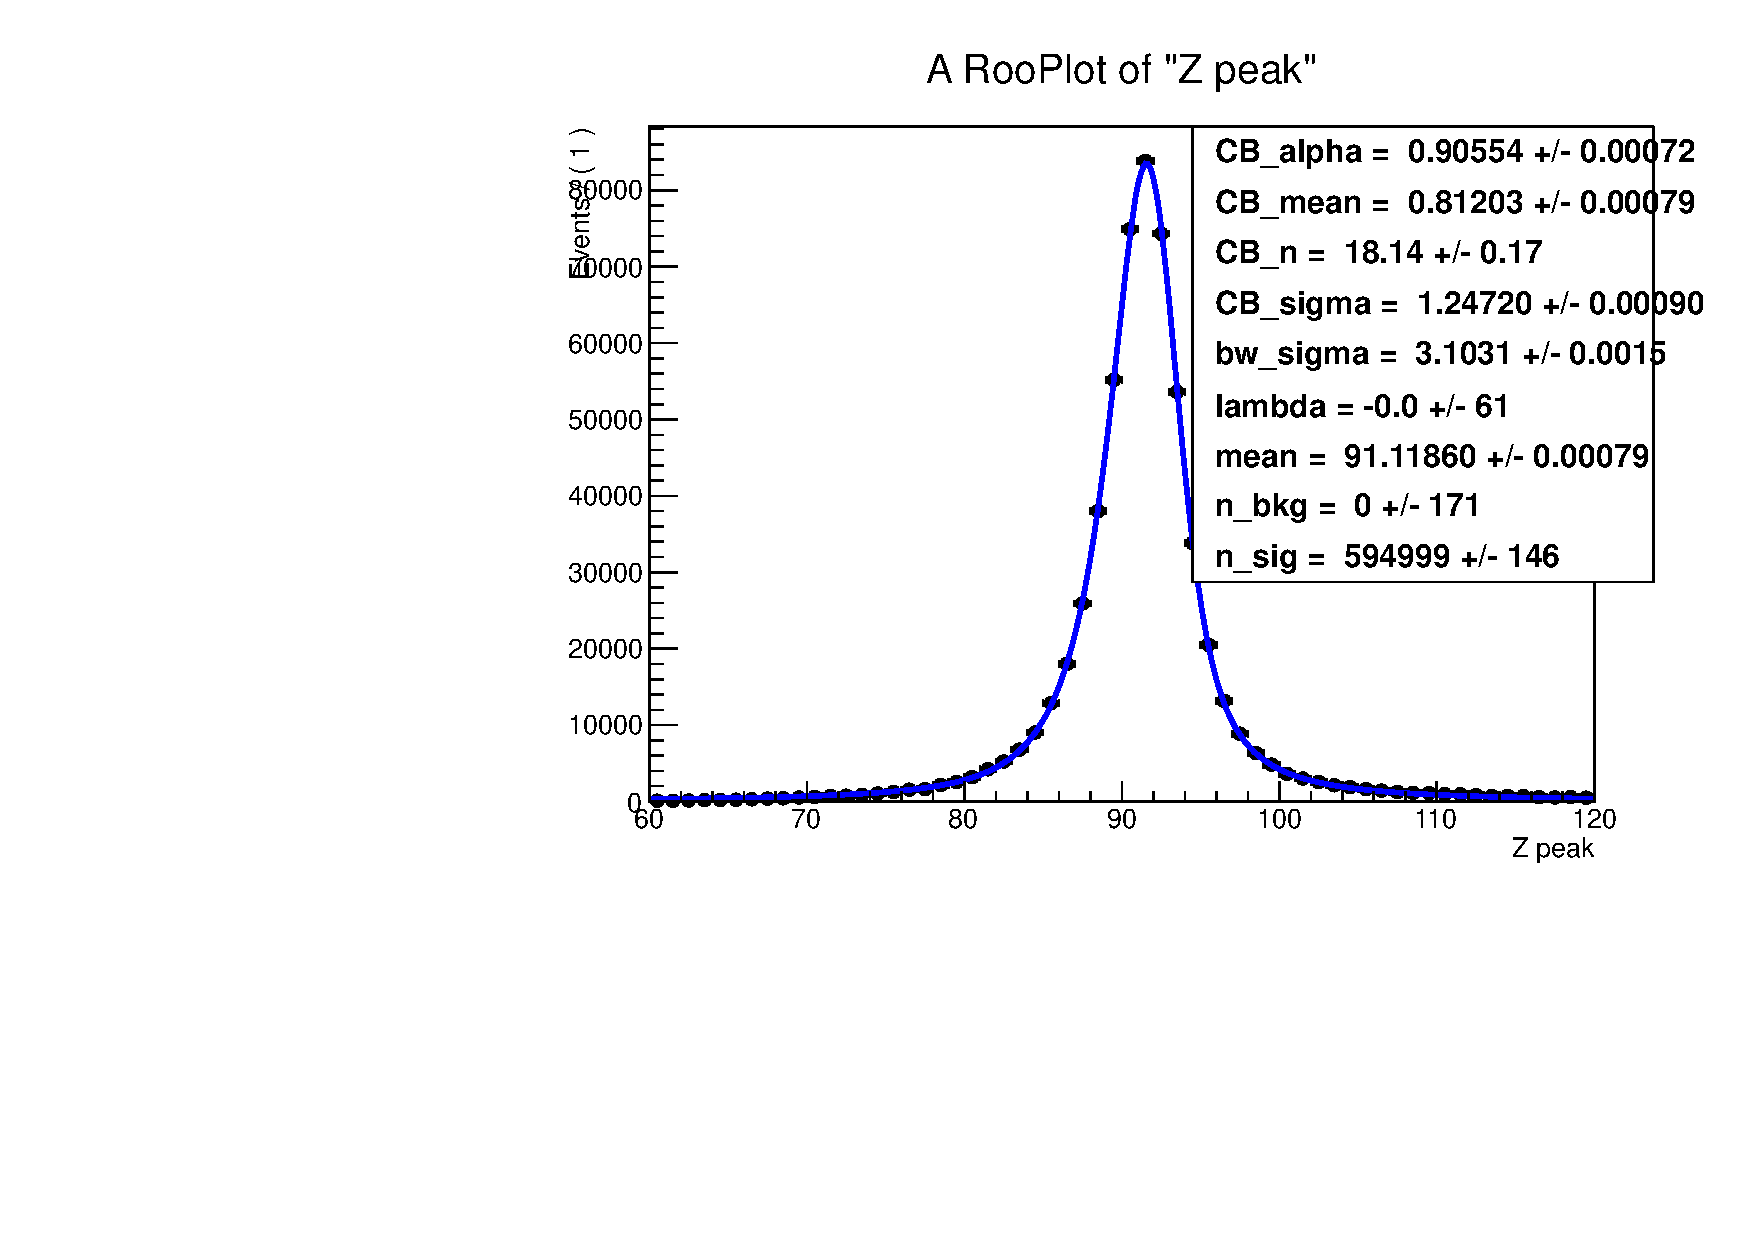
\includegraphics[width=0.48\textwidth]{Chapters/07_08_09_Analysis/Images/lepton_scale_factors/CBConvolution/electron/data/id_iso/tagProbe_passed_Z_peak}\\
     \caption[Fits of the invariant mass distribution of all tag-and-probe pairs and tag-and-probe pairs in
     which the probe satisfies the identification and isolation criteria.]{Fits of the invariant mass
     distribution of all tag-and-probe pairs (left) and tag-and-probe pairs in which the probe satisfies
     the identification and isolation criteria (right).}
     \label{fig:electron_id_iso_efficiency_invariant_Z_mass_fits_data}
\end{figure}

The efficiency of the identification and isolation process is then calculated using the numbers extracted
from the fits, in bins of \pt and $\eta$ of the probe electron, as follows:

\begin{equation}
\epsilon(\text{identification and isolation}) = \frac{N^{\text{fit}}_{\text{probe, passing}}}{N^{\text{fit}}_{\text{probe, all}}}
\end{equation}
where $N^{\text{fit}}_{\text{probe, all}}$ is the total number of events with tag and probe electrons and
$N^{\text{fit}}_{\text{probe, passing}}$ is the subset in which the probe passes identification and isolation
criteria.

The scale factor is then calculated as the ratio between the efficiencies in simulation and in data. The
efficiencies in both can be seen to be similar in Figure~\ref{fig:electron_id_iso_efficiencies_wrt_eta_pt},
leading to scale factors close to one.

\begin{figure}[hbtp]
    \centering
      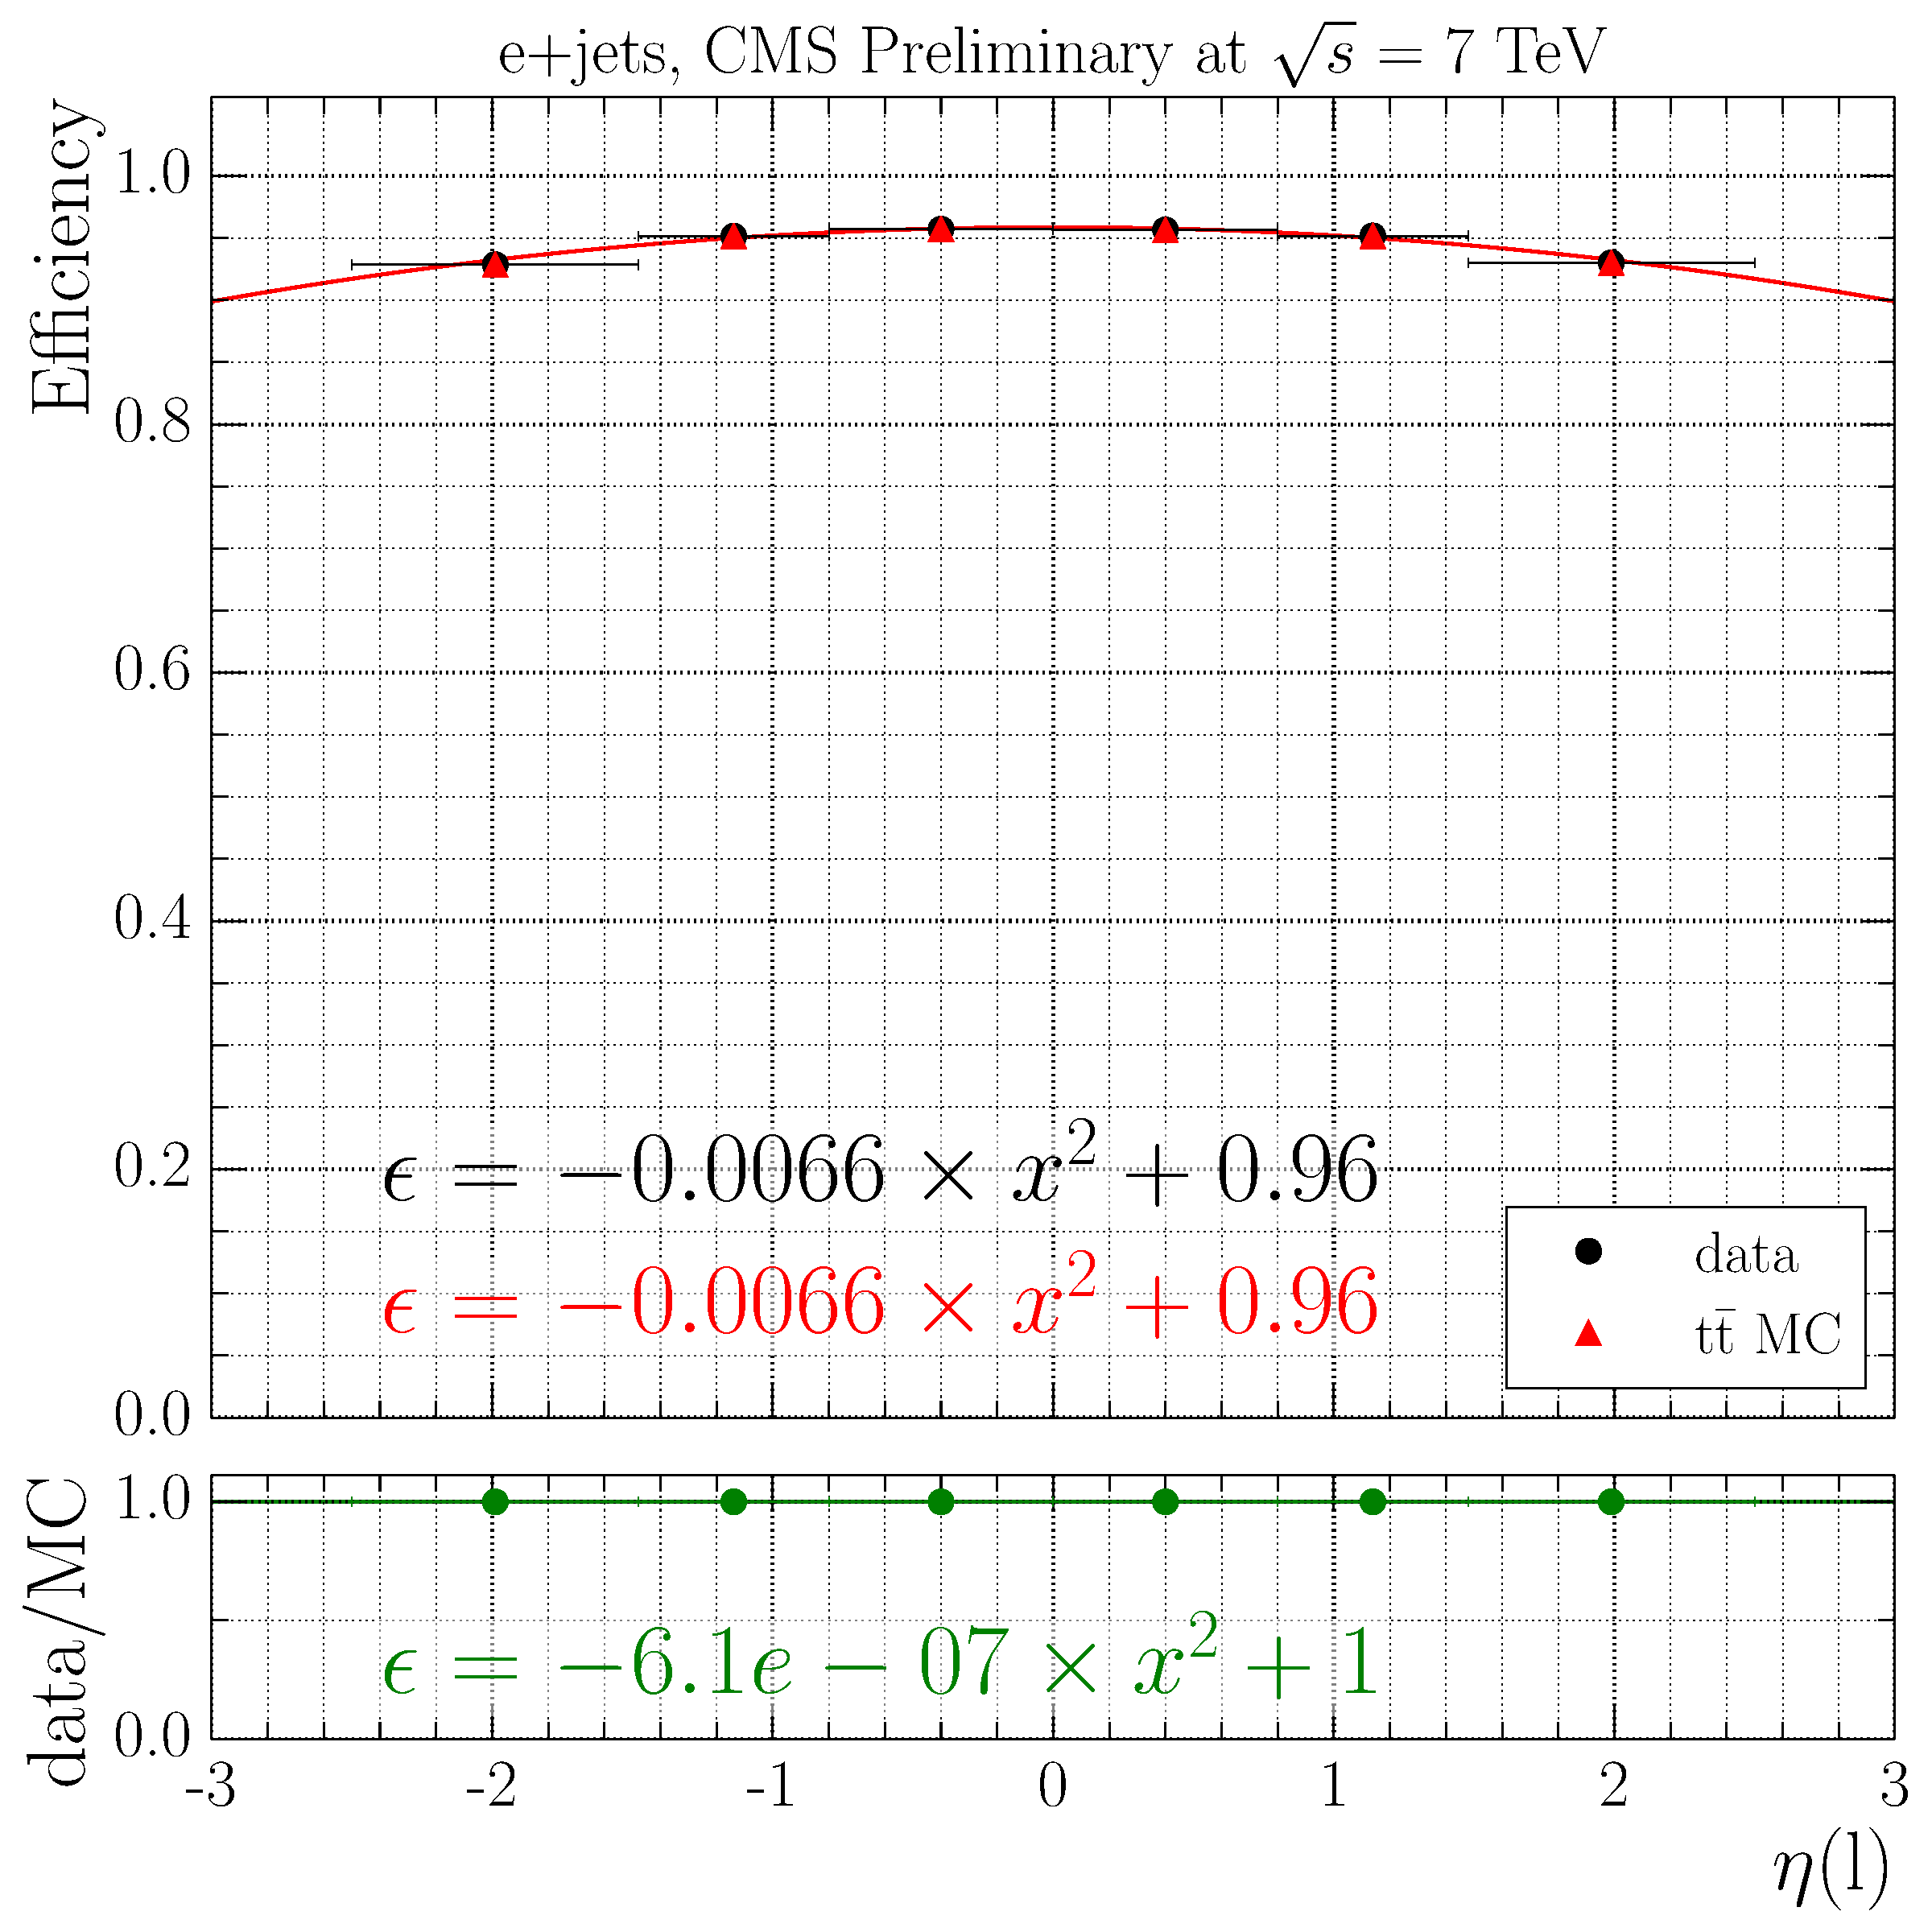
\includegraphics[width=0.48\textwidth]{Chapters/07_08_09_Analysis/Images/lepton_scale_factors/CBConvolution/electron/efficiency_eta_id_iso}\hfill
      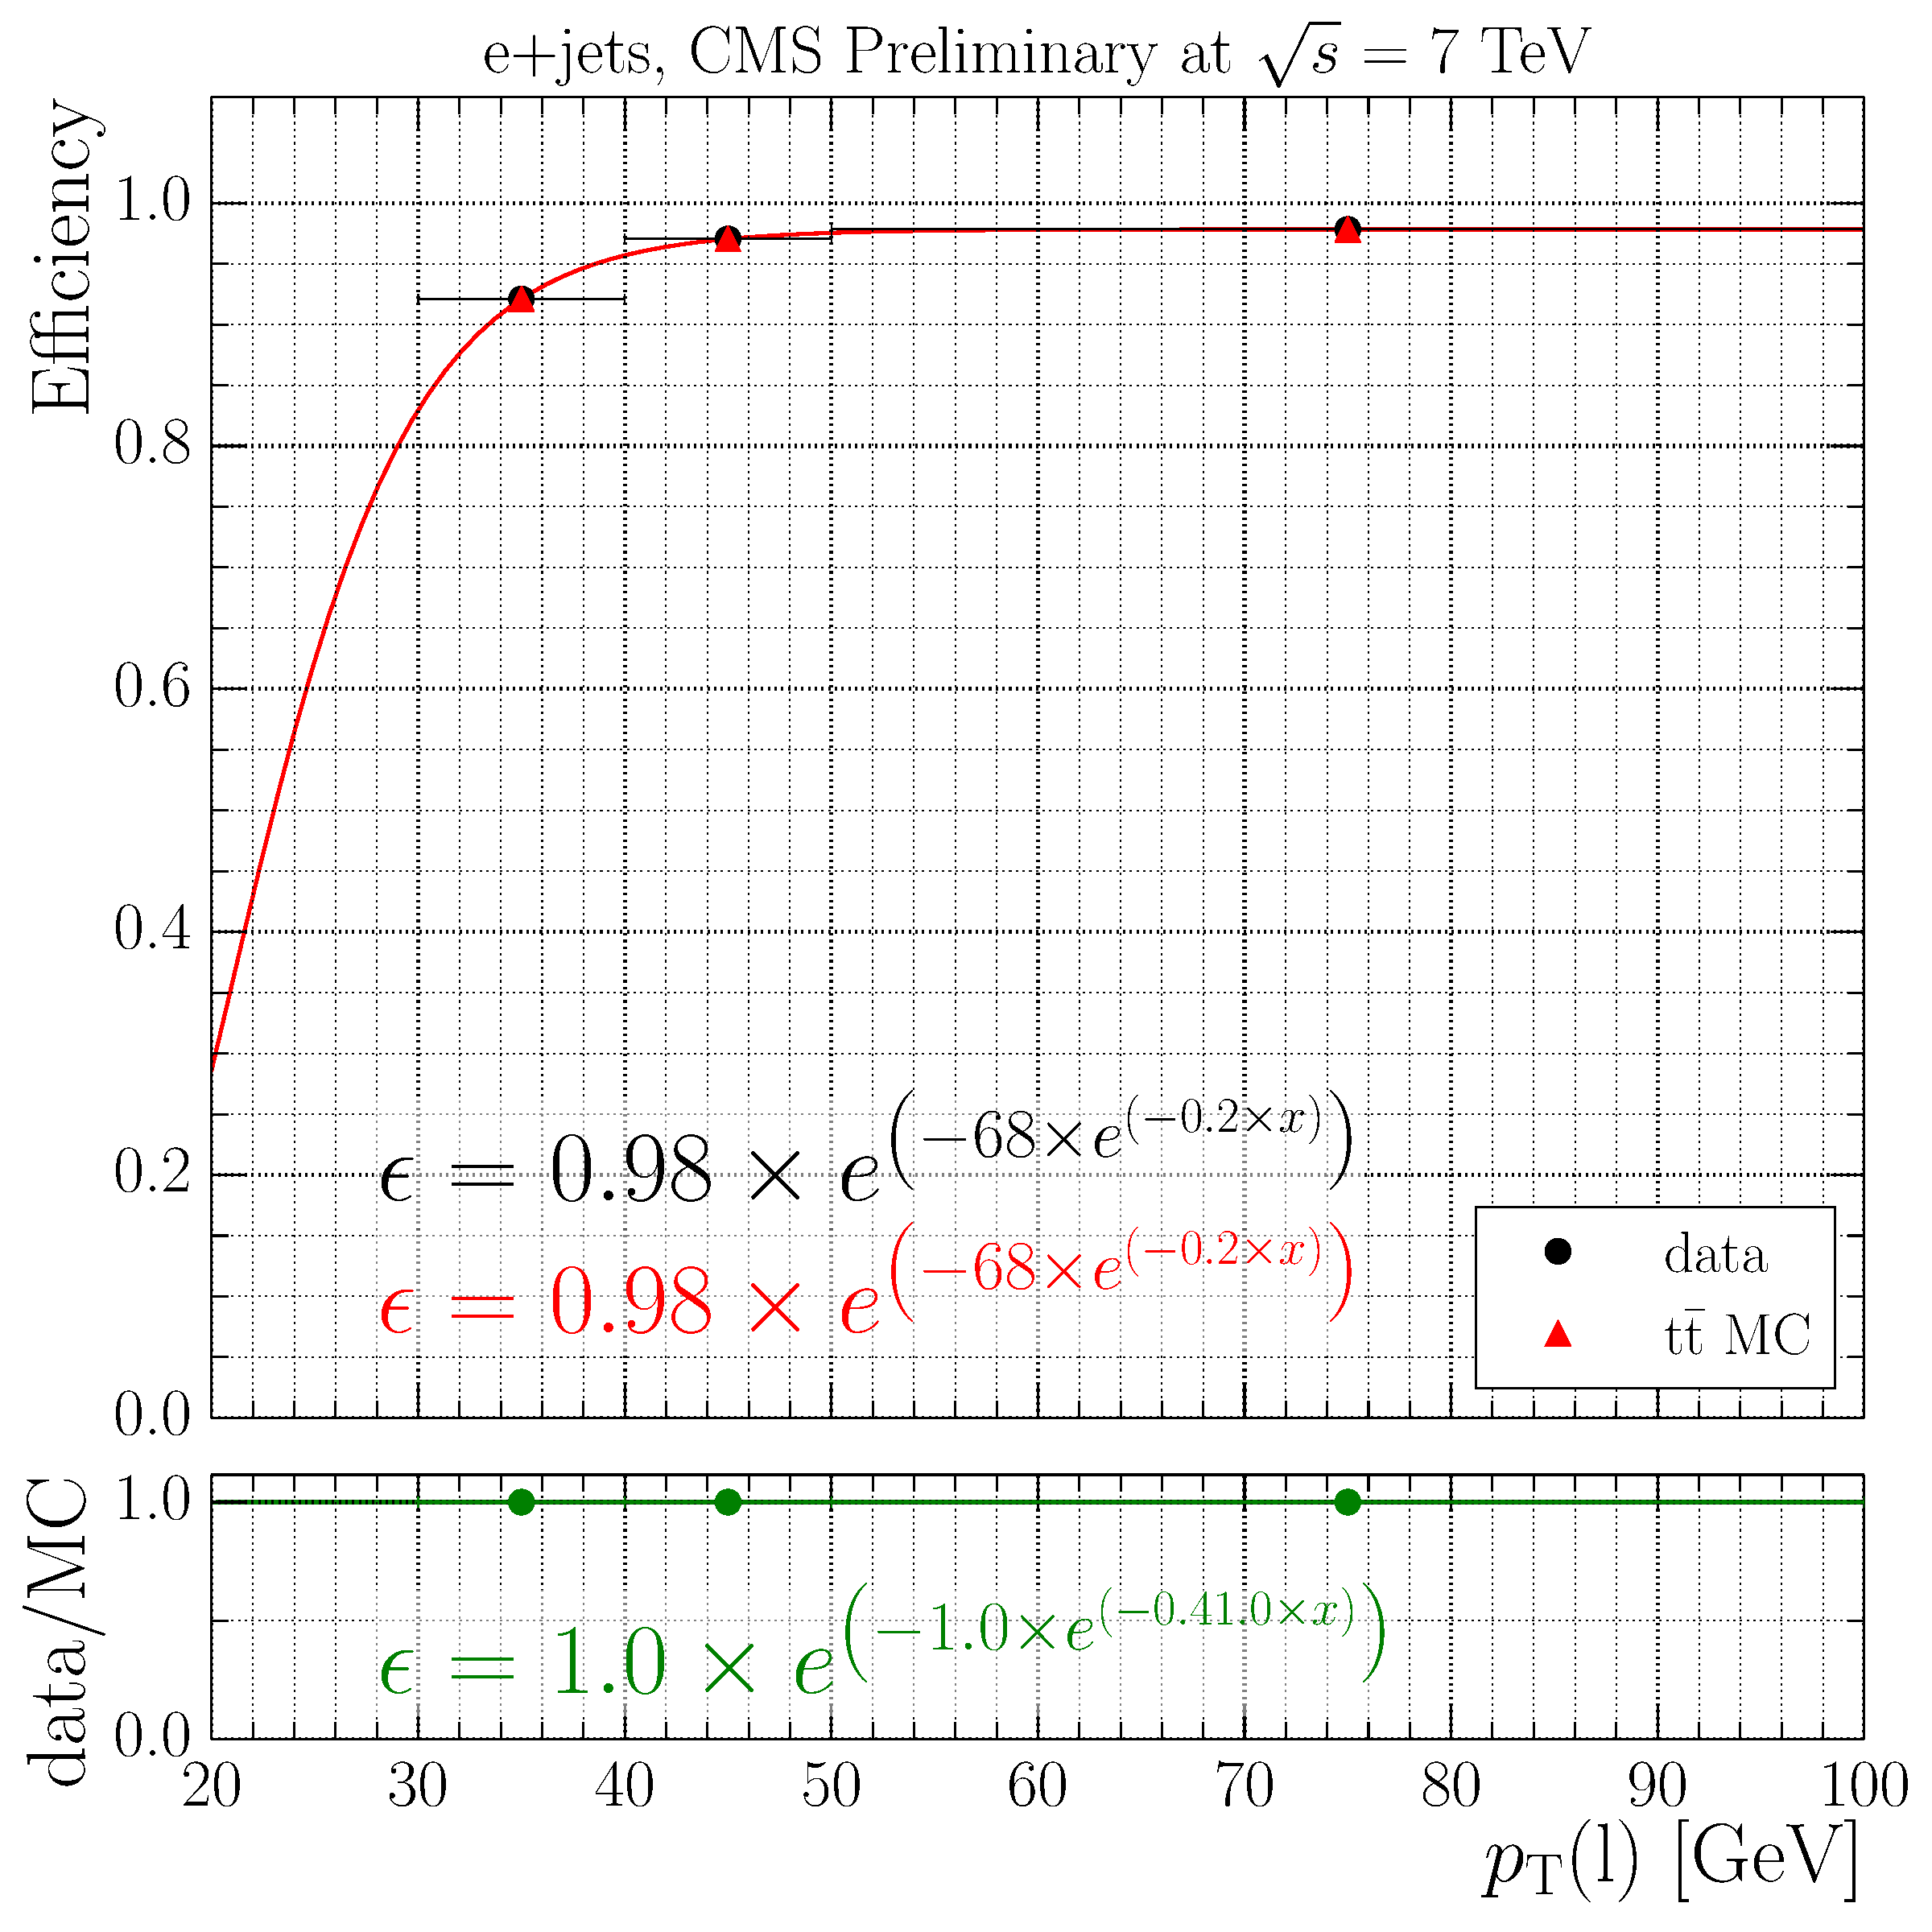
\includegraphics[width=0.48\textwidth]{Chapters/07_08_09_Analysis/Images/lepton_scale_factors/CBConvolution/electron/efficiency_pt_id_iso}
      \caption[Identification and isolation efficiencies as a function of $\eta$ and \pt in data and \ttbar
      Monte Carlo simulation.]{Identification and isolation efficiencies as a function of $\eta$ and \pt in data and \ttbar
      Monte Carlo simulation.}
     \label{fig:electron_id_iso_efficiencies_wrt_eta_pt}
\end{figure}

The efficiency of the electron part of the trigger is then similarly calculated, with respect to the
identification and isolation requirements, meaning the events passing the identification and isolation
requirements in the previous stage are then used as the baseline for the trigger efficiency. The subset of
these in which the probe electron matches a HLT electron is then used to calculate the efficiency as follows:

\begin{equation}
\epsilon(\text{trigger}) = \frac{N^{\text{fit}}_{\text{probe, matching HLT}}}{N^{\text{fit}}_{\text{probe,identification and isolation}}}
\label{eq:electron_leg_efficiency}
\end{equation}
where $N^{\text{fit}}_{\text{probe,identification and isolation}}$ is the number of
events passing from equation~\ref{eq:electron_leg_efficiency} and $N^{\text{fit}}_{\text{probe, matching
HLT}}$ is the subset in which the probe is matched to an HLT electron object.

In order to calculate the efficiency of the hadron leg of the trigger, the full selection with only the
electron part of the trigger and without \btagging, applied to the SingleElectron dataset, is taken as the
baseline. The number of these events passing the hadronic leg of the trigger is then used to calculate the
hadronic leg efficiency as follows:

\begin{equation}
\epsilon(\text{hadron leg}) = \frac{N_{\text{hadron leg, passing}}}{N_{\text{passing selection}}}
\end{equation}
where $N_{\text{passing selection}}$ is the number of events passing the baseline selection with
the electron leg of the trigger and no \btagging requirements, and $N_{\text{hadron leg, passing}}$ is the
subset in which the hadron leg of the trigger is satisfied.

The scale factors are produced in bins of \pt and $\eta$ of the fourth most energetic jet, since this is the
lowest energy jet that is selected. Parametrising as a function of higher energy jets would lead to a bias
towards high efficiencies as the trigger will have a higher efficiency at higher jet energies.

Equivalent fit and efficiency plots for the trigger are included in
Figures~\ref{fig:electron_trigger_efficiency_invariant_Z_mass_fits} and
\ref{fig:electron_trigger_efficiencies_wrt_eta_pt} in Appendix~\ref{as:data_monte_carlo_corrections}.
